%%%%%%%%%%%%%%%%%%%%%%%%%%%%%%%%%%%%%%%%%%%%%%%%%%%%%%%%%%%%%%%%%%%%%%%%%%%%%%%%
% University of Western Ontario Thesis Template
% 1. Initial version by: Justin Quinn Veenstra, 2010 with thanks to Mr. (soon to be Dr.) Will Robertson.
% 2. Adapted by: Dr. John Stuart Haberl Baxter, 2018 for his thesis.
% 3. Dr. Baxter's thesis converted to generic template by: Dr. Jonathan C. Lau, 2018.


\documentclass[hidelinks,12pt,oneside]{report}
%% Decomment next line to use PostScript fonts
%%\UsePackage{times}
%%%%%%%%%%%%%%%%%%%%%%%%%%%%%%%%%%%%%%%%%%%%%%%%%%%%%%%%%%%%%%%%%%%%%%%%
%%                                                                    %%
%%                    ***   I M P O R T A N T   ***                   %%
%%                                                                    %%
%% Fill in the following fields with the required information:        %%
%%  - \department{...}  name of the graduate department               %%
%%  - \degree{...}      name of the degree obtained                   %%
%%  - \author{...}      name of the author                            %%
%%  - \title{...}       title of the thesis                           %%
%%  - \gyear{...}       year of graduation                            %%
%%  - \super{...}    supervisor
%%  - \firstname, \middlename, \lastname... there is additional documentation by the actual fields, so I'll leave it at that
%%%%%%%%%%%%%%%%%%%%%%%%%%%%%%%%%%%%%%%%%%%%%%%%%%%%%%%%%%%%%%%%%%%%%%%%
\usepackage{appendix}
\usepackage{nameref}
\usepackage{hyperref}
\usepackage{graphicx}
\usepackage{amsmath}
\usepackage[byname]{smartref}
\usepackage[]{amssymb}
\usepackage[font=small]{caption}
\usepackage[font=small]{subcaption}
\usepackage{setspace}
\usepackage{enumitem}
\usepackage{lmodern}
\usepackage{booktabs}
\usepackage{rotating}
\usepackage{multirow}
\usepackage{float}
\usepackage{listings}
\usepackage{fancyvrb}  % in your preamble


\newlength\longest
%\usepackage{lineno}%comment out for hardcopy
\usepackage{units}
\usepackage{txfonts}
\usepackage{tocloft}
\usepackage{tabularx}
\usepackage{longtable}
\usepackage{minted}
\usepackage{xcolor}
\definecolor{bg}{rgb}{0.97,0.97,0.97}
%\usepackage[sectionbib]{chapterbib}

\usepackage{hyperref} %comment out for hardcopy
\usepackage{txfonts}
\usepackage{tocloft}
\usepackage{color}
\usepackage{pdfpages}


\makeatletter
\numberwithin{figure}{chapter}
\newenvironment{acknowledgements}%
{\clearemptydoublepage
 \begin{center}
  \section*{Acknowledgements}
 \end{center}
 \begingroup
}{\newpage\endgroup}


\usepackage[boxruled,algochapter]{algorithm2e}

\DeclareMathOperator*{\argmin}{\operatorname{argmin}}
\DeclareMathOperator*{\Proj}{\operatorname{Proj}}
\DeclareMathOperator*{\dvg}{\operatorname{div}}

\newenvironment{dedication}%
{\clearemptydoublepage 
 \begin{center}
  \section*{Dedication}
 \end{center}
 \begingroup
}{\newpage\endgroup}

\newenvironment{preliminary}%
{\pagestyle{plain}\pagenumbering{roman}}%
{\pagenumbering{arabic}}

\addtoreflist{chapter}
\newtheorem{theorem}{Theorem}[section]
\newtheorem{lemma}[theorem]{Lemma}
\newtheorem{proposition}[theorem]{Proposition}
\newtheorem{corollary}[theorem]{Corollary}
\newtheorem{axiom}{Axiom}

\newenvironment{proof}[1][Proof]{\begin{trivlist}
\item[\hskip \labelsep {\bfseries #1}]}{\end{trivlist}}
\newenvironment{definition}[1][Definition]{\begin{trivlist}
\item[\hskip \labelsep {\bfseries #1}]}{\end{trivlist}}
\newenvironment{example}[1][Example]{\begin{trivlist}
\item[\hskip \labelsep {\bfseries #1}]}{\end{trivlist}}
\newenvironment{remark}[1][Remark]{\begin{trivlist}
\item[\hskip \labelsep {\bfseries #1}]}{\end{trivlist}}

\newcommand{\qed}{\nobreak \ifvmode \relax \else
      \ifdim\lastskip<1.5em \hskip-\lastskip
      \hskip1.5em plus0em minus0.5em \fi \nobreak
      \vrule height0.75em width0.5em depth0.25em\fi}

% Default values for title page.

%% To produce output with the desired line spacing, the argument of
%% \spacing should be multiplied by 5/6 = 0.8333, so that 1 1/2 spaced
%% corresponds to \spacing{1.5} and double spaced is \spacing{1.66}.
\def\normalspacing{1.66} % default line spacing


%% Define the "thesis" page style.
\if@twoside % If two-sided printing.
\def\ps@thesis{\let\@mkboth\markboth
   \def\@oddfoot{}
   \let\@evenfoot\@oddfoot
   \def\@oddhead{
      {\sc\rightmark} \hfil \rm\thepage
      }
   \def\@evenhead{
      \rm\thepage \hfil {\sc\leftmark}
      }
   \def\chaptermark##1{\markboth{\ifnum \c@secnumdepth >\m@ne
      Chapter \ \thechapter. \ \fi ##1}{}}
   \def\sectionmark##1{\markright{\ifnum \c@secnumdepth >\z@
      \thesection. \ \fi ##1}}}
\else % If one-sided printing.
\def\ps@thesis{\let\@mkboth\markboth
   \def\@oddfoot{}
   \def\@oddhead{
      {\sc\rightmark} \hfil \rm\thepage
      }
   \def\chaptermark##1{\markright{\ifnum \c@secnumdepth >\m@ne
      Chapter\ \thechapter. \ \fi ##1}}}
\fi

\if@twoside % If two-sided printing.
\def\ps@appendix{\let\@mkboth\markboth
   \def\@oddfoot{}
   \let\@evenfoot\@oddfoot
   \def\@oddhead{
      {\sc\rightmark} \hfil \rm\thepage
      }
   \def\@evenhead{
      \rm\thepage \hfil {\sc\leftmark}
      }
   \def\chaptermark##1{\markboth{\ifnum \c@secnumdepth >\m@ne
      Appendix \ \thechapter. \ \fi ##1}{}}
   \def\sectionmark##1{\markright{\ifnum \c@secnumdepth >\z@
      \thesection. \ \fi ##1}}}
\else % If one-sided printing.
\def\ps@thesis{\let\@mkboth\markboth
   \def\@oddfoot{}
   \def\@oddhead{
      {\sc\rightmark} \hfil \rm\thepage
      }
   \def\chaptermark##1{\markright{\ifnum \c@secnumdepth >\m@ne
      Chapter\ \thechapter. \ \fi ##1}}}
\fi

\pagestyle{thesis}
% Set up page layout.
\setlength{\textheight}{9in} % Height of the main body of the text
\setlength{\topmargin}{-.5in} % .5" margin on top of page
\setlength{\headsep}{.5in}  % space between header and top of body
\addtolength{\headsep}{-\headheight} % See The LaTeX Companion, p 85
\setlength{\footskip}{.5in}  % space between footer and bottom of body
\setlength{\textwidth}{6.25in} % width of the body of the text
\setlength{\oddsidemargin}{.25in} % 1.25" margin on the left for odd pages
\setlength{\evensidemargin}{0in} % 1.25"  margin on the right for even pages

% Marginal notes
\setlength{\marginparwidth}{.75in} % width of marginal notes
\setlength{\marginparsep}{.125in} % space between marginal notes and text

% Make each page fill up the entire page. comment this out if you
% prefer. 
\flushbottom

\setcounter{tocdepth}{3} % Number the subsubsections 
\def\normalspacing{1.66} % default line spacing

\newcommand\isco[1]{%
  \edef\@tempa{#1}%
  \def\@tempb{}%
  \ifx\@tempa\@tempb
	\else \\\underline{Co-Supervisor:}\vspace{0.35in}\\\dots\dots\dots\dots\dots\dots\dots\\{#1}\\
  \fi
}

\newcommand\isjoint[1]{%
  \edef\@tempa{#1}%
  \def\@tempb{}%
  \ifx\@tempa\@tempb
	\else \\\underline{Joint Supervisor:}\vspace{0.35in}\\\dots\dots\dots\dots\dots\dots\dots\\{#1}\\
  \fi
}

\newcommand\isalt[1]{%
  \edef\@tempa{#1}%
  \def\@tempb{}%
  \ifx\@tempa\@tempb
	\else \\\underline{Alternate Supervisor:}\vspace{0.35in}\\\dots\dots\dots\dots\dots\dots\dots\\{#1}\\
  \fi
}

\newcommand\isdefinedsig[1]{%
  \edef\@tempa{#1}%
  \def\@tempb{}%
  \ifx\@tempa\@tempb
	\else \\ \dots\dots\dots\dots\dots\dots\dots\\{#1}\\
  \fi
}
\newcommand\isdefinedspinetitle[1]{%
  \edef\@tempa{#1}%
  \def\@tempb{}%
  \ifx\@tempa\@tempb
	\else (Spine title: #1)\\
  \fi
}
\newcommand\coauthor[1]{%
  \edef\@tempa{#1}%
  \def\@tempb{}%
  \ifx\@tempa\@tempb
	\else \newpage \Large Co-Authorship Statement\normalsize\\\indent\\#1\\
  \fi
}

\newcommand\acknowlege[1]{%
  \edef\@tempa{#1}%
  \def\@tempb{}%
  \ifx\@tempa\@tempb
	\else \newpage \Large Acknowledgements\normalsize\\\indent\\#1\newpage
  \fi
}

%\renewcommand{\appendixtocname}{\Huge \textbf{List of Appendices} \normalsize}
\newcommand{\blank}{\hspace{-2mm}}
\newcommand{\super}{Dr. Supervisor1} %supervisor
\newcommand{\superj}{Dr. Supervisor2} %joint supervisor, if there is one, leave blank if not (lbin)... only one of the three.
\newcommand{\superc}{} %co-supervisor, if there is one, leave blank if not (lbin)
\newcommand{\supera}{} %alternate supervisor, if there is one, leave blank if not (lbin)
\newcommand{\scoa}{Dr. Committee1}  %member of supervisory committee
\newcommand{\scob}{Dr. Committee2}  %member of supervisory committee
\newcommand{\scoc}{Dr. Committee3}  %member of supervisory committee
\newcommand{\sct}{}  %other member of supervisory committee (lbin)
\newcommand{\examo}{Dr. Examiner1}  %examining committee (up to four, if less leave blank)
\newcommand{\examt}{Dr. Examiner2}
\newcommand{\examth}{Dr. Examiner3}
\newcommand{\examf}{Dr. Examiner4}
\newcommand{\department}{School of Biomedical Engineering}
\newcommand{\degree}{Doctor of Philosophy}
\newcommand{\firstname}{Alaa}
\newcommand{\middlename}{}
\newcommand{\lastname}{Taha}
%\renewcommand{\author}[1]{\ifx\empty#1\else\gdef\@author{#1}\fi} 
\newcommand{\authorname}{{\firstname} {\middlename} {\lastname}}
\newcommand{\titl}{Bridging coordinates and machine learning for brain mapping and stereotaxy}
\newcommand{\spinetitle}{}%only if the above is more than 60 characters
\newcommand{\thesisformat}{Integrated Article} %or Monograph
\newcommand{\gyear}{\number\year}
\newcommand{\makecoauthor}{}
\newcommand{\makeacknowlege} {
%Type in acknowlegements here
}
\newcommand{\listappendixname}{List of Appendices}
\newlistof{myappendices}{app}{\listappendixname}
\newcommand{\myappendices}[1]{%
\addcontentsline{app}{myappendices}{#1}\par}

\renewcommand{\maketitle}
{\begin{titlepage}
   \setcounter{page}{1}
   %% Set the line spacing to 1 for the title page.
   %\begin{spacing}{1} 
   \begin{large}
   \begin{center}
      \mbox{}
      \vfill
      {\MakeUppercase{\titl}}\\
      \isdefinedspinetitle{\spinetitle}
      (Thesis format: \thesisformat)\\
      \vfill
      by \\
      \vfill
      {\firstname{} \middlename } \underline{\lastname}\\
      \vfill
      Graduate Program in {\department}\\
      \vfill
		A thesis submitted in partial fulfillment\\
		of the requirements for the degree of\\
		\degree\\
		\vfill
		The School of Graduate and Postdoctoral Studies\\
		The University of Western Ontario\\
		London, Ontario, Canada\\
		\vfill
      {\copyright} {\authorname} {\gyear}  \\
      \vspace*{.2in}
   \end{center}
   \end{large}
%   \end{spacing}
   \end{titlepage}

}%\maketitle

\newcommand{\makecert}{
   \setcounter{page}{2}
\vfill
\begin{center}
\large
THE UNIVERSITY OF WESTERN ONTARIO\\
School of Graduate and Postdoctoral Studies\\
\vfill
\textbf{CERTIFICATE OF EXAMINATION}
\end{center}

\vfill
\begin{table}[ht]
\begin{minipage}[t]{0.5\linewidth} %tabular instead?
\begin{tabular}{l}
\underline{Supervisor:}\vspace{0.35in}
\isdefinedsig{\super}
\isco{\superc}
\isjoint{\superj}
\isalt{\supera}
\\
%\underline{Supervisory Committee:}\vspace{0.35in}
%\isdefinedsig{\scoa}\vspace{0.15in}
%\isdefinedsig{\scob}\vspace{0.15in}
%\isdefinedsig{\scoc}\vspace{0.15in}
%\isdefinedsig{\sct}
\end{tabular}
\vfill
\end{minipage}
\hspace{0.5in}
\begin{minipage}[t]{0.5\linewidth}
\begin{tabular}{l}
\underline{Examiners:} \\\vspace{.5cm}
\isdefinedsig{\examo}\\
\isdefinedsig{\examt}\\
\isdefinedsig{\examth}\\
\isdefinedsig{\examf}
\end{tabular}
\vfill
\end{minipage}
\vfill
\end{table}
\vfill
\begin{center}
The thesis by \\ \vfill
\textbf{\firstname{} \middlename{} \underline{\lastname}}\\
\vfill
entitled:\\\vfill
\textbf{\titl}\\\vfill
is accepted in partial fulfillment of the \\
requirements for the degree of\\
\degree\\
\end{center}
\begin{table}[ht]
\begin{minipage}[t]{0.5\linewidth}
\begin{tabular}{l}
\dots\dots\dots\dots\dots\\
Date
\end{tabular}
\end{minipage}
\hspace{0.5in}
\begin{minipage}[t]{0.5\linewidth}
\begin{tabular}{l}
\dots\dots\dots\dots\dots\dots\dots\dots\dots\dots\\
Chair of the Thesis Examination Board
\end{tabular}
\end{minipage}
\end{table}

}

\makeatother
\begin{document}


%% ***   NOTE   ***
%% You should put all of your '\newcommand', '\newenvironment', and
%% '\newtheorem's (in other words, all the global definitions that you
%% will need throughout your thesis) in a separate file and use
%% "\input{filename}" to input it here.


%% This sets the page style and numbering for preliminary sections.
\begin{preliminary}

%% This generates the title page from the information given above.
\maketitle
%\addcontentsline{toc}{chapter}{Certificate of Examination}
%\makecert
%\addcontentsline{toc}{chapter}{Acknowlegements}
%\acknowlege{\makeacknowlege}	%as above
\setcounter{page}{2}
\phantomsection
\addcontentsline{toc}{chapter}{Abstract}
\Large\begin{center}\textbf{Abstract}\end{center}\normalsize
\onehalfspacing

Stereotactic neurosurgery involves the precise targeting of brain structures—where millimetric deviations can mean the difference between optimal therapy and adverse outcomes. Deep brain stimulation (DBS) is a stereotactic procedure that involves electrode implantation into subcortical brain regions to modulate dysfunctional neural circuits. Enabled by advances in neuroimaging and surgical technology, DBS has been applied across a broad range of neurological and psychiatric disorders, with over 250,000 cases performed worldwide. However, millimetric localization of small subcortical regions can be challenging. Clinical MRI is often limited by resolution, contrast, and artifacts, while nonlinear registration—considered the gold standard for automatic localization—yields errors ranging from 1 to 5 millimeters. Errors in this range can be clinically meaningful given the anatomical and functional complexity of DBS targets. As a result, there is growing demand for tools that enable millimetric localization across imaging modalities and patient populations. Developments in machine learning (ML) offer opportunities to address challenges in brain structure localization by improving accuracy, automation, and scalability but require validation to meet the spatial demands of neurosurgical targeting. This dissertation leverages brain coordinates inspired by classical stereotactic principles and ML to develop open software infrastructure that supports spatially precise and interpretable workflows in neuroimaging and neurosurgery. In \textbf{Chapter \ref{chap:afidsdata}}, we validate a protocol for brain landmark annotation and openly release 6,000 coordinates placed on structural MRI across multiple field strengths and clinical populations. We demonstrate the utility of this protocol and data for millimetric quality control of neuroimaging workflows. In \textbf{Chapter \ref{chap:AutoAFIDs}}, we use this data to develop \texttt{AutoAFIDs}, an open-source application for automatic landmark detection that achieves millimetric localization accuracy. We showcase the broader utility of \texttt{AutoAFIDs} by building modular applications for registration quality control and morphometric brain charting. In \textbf{Chapter \ref{chap:afidspred}}, we extend this coordinate-based framework to predict the location of the most common DBS target called the subthalamic nucleus, demonstrating millimetric accuracy on clinical MRI and validate predictions using ultra-high field MRI where ground truth anatomy is visible. Together, the tools developed in this dissertation establish an open and generalizable infrastructure for surgical targeting, image validation, and population-level brain mapping.


\vfill
\noindent\textbf{Keywords:} stereotactic neurosurgery, deep brain stimulation, brain coordinates, machine learning, magnetic resonance imaging, image registration, surgical targeting, quality control, open-source.
\newpage


\clearpage
\phantomsection
\addcontentsline{toc}{chapter}{Summary for Lay Audience}
\Large\begin{center}\textbf{Summary for Lay Audience}\end{center}\normalsize

\onehalfspacing



\vfill
\newpage

\phantomsection
\addcontentsline{toc}{chapter}{Co-Authorship Statement}
\Large\begin{center}\textbf{Co-Authorship Statement}\end{center}\normalsize
\setstretch{1.4}

\noindent \textbf{Chapter 1: Introduction }\\
\hangindent=1.2cm A. Taha — Sole author

\vspace{0.5em}

\noindent \textbf{Chapter 2: MRI Datasets with Anatomical Fiducial Annotations}\\
\hangindent=1.2cm A. Taha — Conceptualization, Methodology, Software, Validation, Formal Analysis, Visualization, Writing – Original Draft \\
\hangindent=1.2cm J. C. Lau, A. R. Khan — Conceptualization, Supervision, Funding Acquisition, Resources, Writing – Review and Editing \\
\hangindent=1.2cm All Authors — Software, Data Curation, Writing – Review and Editing

\vspace{0.5em}

\noindent \textbf{Chapter 3: Automatic Anatomical Fiducial Localization}\\
\hangindent=1.2cm A. Taha — Conceptualization, Methodology, Software, Validation, Formal Analysis, Visualization, Writing – Original Draft \\
\hangindent=1.2cm J. C. Lau, A. R. Khan — Conceptualization, Supervision, Funding Acquisition, Resources, Writing – Review and Editing \\
\hangindent=1.2cm D. Bansal, M. Snyder, T. Kuehn, J. Kai, G. Gilmore, A. Thurairajah — Software, Methodology, Validation \\
\hangindent=1.2cm All Authors — Data Curation, Writing – Review and Editing

\vspace{0.5em}

\noindent \textbf{Chapter 4: Stereotactic Target Localization Using Anatomical Fiducials}\\
\hangindent=1.2cm A. Taha — Conceptualization, Methodology, Software, Validation, Formal Analysis, Visualization, Writing – Original Draft \\
\hangindent=1.2cm J. C. Lau, A. R. Khan — Conceptualization, Supervision, Funding Acquisition, Resources, Writing – Review and Editing \\
\hangindent=1.2cm D. Bansal, M. Snyder — Software \\
\hangindent=1.2cm All Authors — Data Curation, Writing – Review and Editing

\vspace{0.5em}

\noindent \textbf{Chapter 5: Conclusions and Future Directions}\\
\hangindent=1.2cm A. Taha — Sole author

\vfill
\newpage
\thispagestyle{empty}
\vspace*{\fill}

\begin{flushleft}
\hspace{3cm}
\begin{minipage}{0.6\textwidth}
\setstretch{1} 
  {\Large\itshape
  We shall not cease from exploration\\
  And the end of all our exploring\\
  Will be to arrive where we started\\
  And know the place for the first time.\par\bigskip}
  \hfill\MakeUppercase{--T.S. Eliot}\\
  \hfill\textit{“Little Gidding”, Four Quartets}
\end{minipage}
\end{flushleft}

\vspace*{\fill}
\newpage



\phantomsection
\addcontentsline{toc}{chapter}{Acknowledgments}
\Large\begin{center}\textbf{Acknowledgments}\end{center}\normalsize
TODO.
\vfill
\newpage
\singlespacing


\tableofcontents\newpage

\newpage
\phantomsection
\addcontentsline{toc}{chapter}{List of Figures}
\begingroup
\sloppy
\setlength{\cftbeforefigskip}{4.5pt}  % adds small space between entries
\listoffigures
\endgroup

\newpage
\phantomsection
\addcontentsline{toc}{chapter}{List of Tables}
\begingroup
\sloppy
\setlength{\cftbeforefigskip}{4pt}  % adds small space between entries
\listoftables
\endgroup

\newpage
\phantomsection
\addcontentsline{toc}{chapter}{List of Appendices}
\listofmyappendices\newpage

\phantomsection
\addcontentsline{toc}{chapter}{List of Abbreviations, Symbols, and Nomenclature}
\Large \textbf{List of Abbreviations, Symbols, and Nomenclature} \normalsize


\begin{longtable}{lcl}
\endfirsthead

\multicolumn{3}{l}{\textbf{List of Abbreviations and Nomenclature (continued)}} \\
\endhead

\endfoot

\multicolumn{3}{l}{\textbf{General Terminology}} \\
3D & & Three-dimensional \\
7T & & Seven Tesla \\
AC & & Anterior commissure \\
PC & & Posterior commissure \\
AC-PC & & Anterior–posterior commissure \\
BG & & Basal ganglia \\
CNR & & Contrast-to-noise ratio \\
CSF & & Cerebrospinal fluid \\
DBS & & Deep brain stimulation \\
GM & & Gray matter \\
IC & & Internal capsule \\
PD & & Parkinson’s disease \\
AD & & Alzheimer's disease \\
RN & & Red nucleus \\
ROI & & Region of interest \\
SNR & & Signal-to-noise ratio \\
STN & & Subthalamic nucleus \\
VTA & & Volume of tissue activated \\
WM & & White matter \\
ZI & & Zona incerta \\
DISTAL & & DBS Intrinsic Template AtLas \\
\\
\multicolumn{3}{l}{\textbf{Medical Imaging Terminology}} \\
BIDS & & Brain Imaging Data Structure \\
MRI & & Magnetic resonance imaging \\
CT & & Computed tomography \\
DICOM & & Digital Imaging and Communications in Medicine \\
DTI & & Diffusion tensor imaging \\
DWI & & Diffusion-weighted imaging \\
FGATIR & & Fast Gray Matter Acquisition T1 Inversion Recovery \\
FLAIR & & Fluid-attenuated inversion recovery \\
MP2RAGE & & Magnetization-prepared 2 rapid gradient echoes \\
MPRAGE & & Magnetization-prepared rapid acquisition gradient echo \\
NIfTI & & Neuroimaging Informatics Technology Initiative \\
NMR & & Nuclear magnetic resonance \\
QSM & & Quantitative susceptibility mapping \\
SPACE & & Sampling Perfection with Application-optimized Contrasts using flip angle Evolutions \\
SWI & & Susceptibility-weighted imaging \\
T1w & & T1-weighted \\
T2w & & T2-weighted \\
TE & & Echo time \\
TI & & Inversion time \\
TR & & Repetition time \\
UHF & & Ultra-high field \\
\\
\multicolumn{3}{l}{\textbf{Machine Learning and Image Processing Terminology}} \\
GPU & & Graphics processing units \\
ANN & & Artificial neural network \\
CNN & & Convolutional neural network \\
DL & & Deep learning \\
MSE & & Mean squared error \\
ED & & Euclidean distance \\
ML & & Machine learning \\
nnU-Net & & No-new-Unet (self-configuring U-Net) \\
ReLU & & Rectified linear unit \\
XGBoost & & Extreme Gradient Boosting \\
ANTs & & Advanced Normalization Tools \\
FLIRT & & FMRIB's Linear Image Registration Tool \\
FNIRT & & FMRIB's Nonlinear Image Registration Tool \\
MI & & Mutual information \\
NCC & & Normalized cross-correlation \\
SSD & & Sum of squared differences \\
SyN & & Symmetric normalization \\
\\
\multicolumn{3}{l}{\textbf{Terms Introduced by this Thesis}} \\
AFID & & Anatomical fiducial \\
AFLE & & Anatomical fiducial localization error \\
AFRE & & Anatomical fiducial registration error \\
\end{longtable}


\newpage
	
\clearpage


\end{preliminary}
%% End of the preliminary sections: reset page style and numbering.

%%%%%%%%%%%%%%%%%%%%%%%%%%%%%%%%%%%%%%%%%%%%%%%%%%%%%%%%%%%%%%%%%%%%%%%%
%%                                                                    %%
%%                    ***   I M P O R T A N T   ***                   %%
%%                                                                    %%
%% Put your Chapters here; the easiest way to do this is to keep each %%
%% chapter in a separate file and \include all the files right here.  %%
%% Note that each chapter file should start with the line             %%
%% "\chapter{ChapterName}".  Note that using "\include" instead of    %%
%% "\input" makes each chapter start on a new page.                   %%
%%%%%%%%%%%%%%%%%%%%%%%%%%%%%%%%%%%%%%%%%%%%%%%%%%%%%%%%%%%%%%%%%%%%%%%%

\onehalfspacing
\chapter{Introduction}\label{chap:intro}
\newpage
\sloppy

Neurosurgical procedures such as deep brain stimulation (DBS) involve targeting small, deep brain structures where spatial deviations of only 1 to 2 millimeters (mm) can be the difference between optimal therapeutic efficacy and adverse effects \cite{Horn2018-qq}. This level of precision highlights a fundamental challenge in neuroimaging: the need for millimetric localization of brain structures despite inter-individual anatomical variability, differences across imaging modalities, imaging artifacts, and imaging sessions.

Precise localization of brain structures remains challenging using clinical neuroimaging \cite{Boutet2021-vg}. Some targets may be difficult to locate due to their small size, limited contrast, susceptibility to artifacts, or inter-individual anatomical variability \cite{Lau2020-dh}. Manual localization can be time consuming and subject to observer variability \cite{Miller2023-ct}. Additional tools are needed to improve accuracy, especially in applications that span imaging modalities, populations, and clinical contexts. Recent developments in machine learning (ML) offer opportunities to address challenges in brain structure localization by improving accuracy, automation, and scalability \cite{Andrews2025-kd}.

This dissertation leverages brain coordinates and ML to develop an open software infrastructure that supports spatially precise and interpretable workflows in neuroimaging and neurosurgery. We investigate how ML-driven brain landmark localization can support millimetric image alignment quality control, enhance surgical targeting workflows, and facilitate population-level morphometric analysis.

In this introductory chapter, we begin with a historical overview of stereotactic neurosurgery and the development of coordinate-based targeting. We present the foundations of magnetic resonance imaging (MRI) and highlight advances in acquisitions, including ultra-high-field MRI. A brief overview of image registration is also discussed, followed by an introduction of coordinate-based frameworks for quantifying alignment and modeling brain structure. Finally, we discuss ML algorithms relevant to this dissertation and outline recent advances to improve the automation and scalability of brain structure localization.

\section{Stereotactic Neurosurgery}
\label{sec:SNSX}
Stereotactic neurosurgery is a subspecialty of neurosurgery dedicated to targeting brain structures for diagnostic or therapeutic purposes. The word stereotaxy is derived from the Greek words “stereos-”, for three-dimensional (3D), and “-taxy”, for arrangement first used by Horsley and Clarke in 1908 \cite{Horsley1908-om}. Central to this approach is the accurate localization of intracranial targets within a standardized 3D space. Early stereotactic innovations (Figure \ref{fig:ch1_Figure_stereoframe}) enabled clinicians and researchers to consistently identify, compare, and intervene in specific regions of the brain, which is central to many brain mapping applications.

\begin{figure}[hbt!]
    \centering
    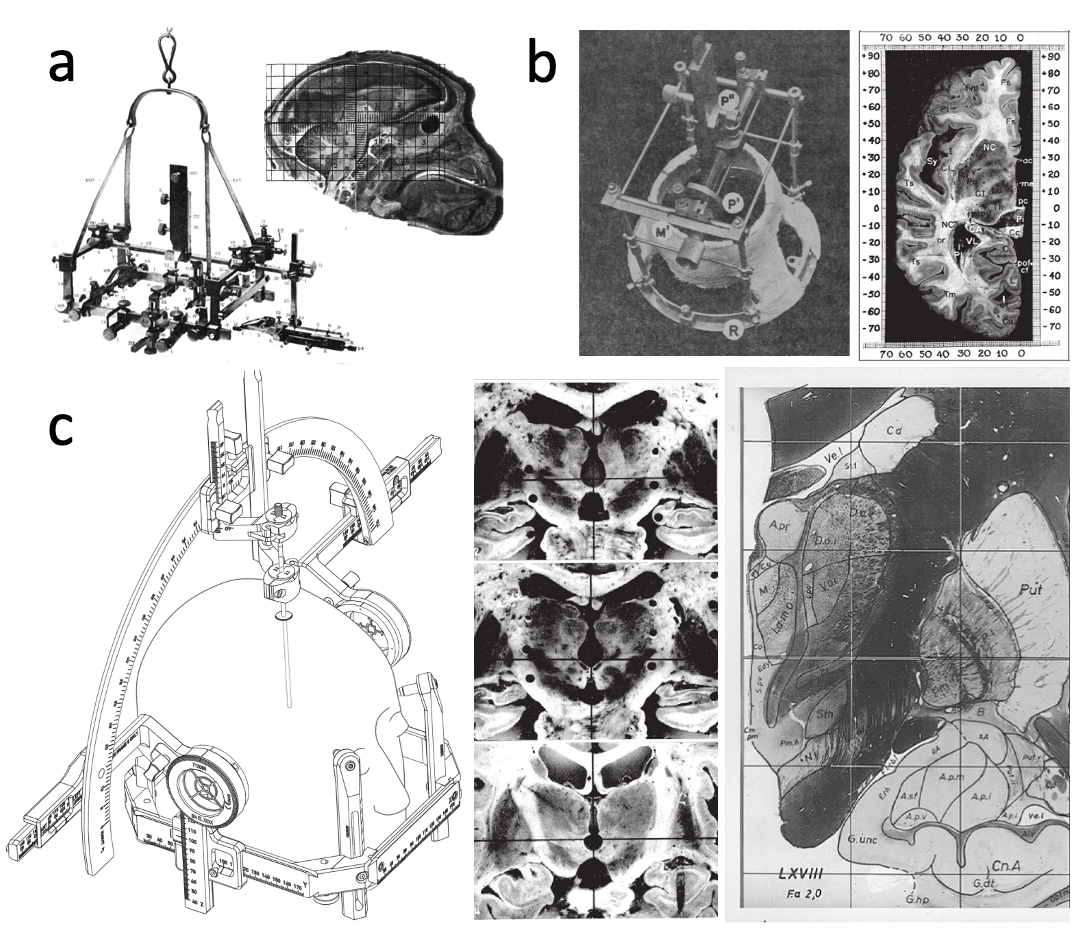
\includegraphics[width=0.85\linewidth]{figs/ch1_Figure_stereoframe.png}
    \caption{Key innovations in stereotactic neurosurgery and their associated reference spaces. (a) Horsley and Clarke’s \cite {Horsley1908-om} frame for cerebellar research, shown with their accompanying atlas. (b) Model V, the frame by Spiegel and Wycis \cite{Spiegel1947-rq} for human brain interventions, alongside their post-mortem reference brain. (c) Modern Leksell-style frame used in clinical practice, shown with common atlases such as Talairach \cite{Talairach1957-eb} and Schaltenbrand \cite{Schaltenbrand1977-ge}.}
    \label{fig:ch1_Figure_stereoframe}
\end{figure}

\subsection{Overview of Stereotactic Neurosurgery}
Victor Horsley and Robert Clarke introduced the first stereotactic apparatus for experimental neurophysiology in non-human primates \cite{Horsley1908-om}. Their system employed a Cartesian coordinate frame anchored to external cranial landmarks, allowing for reproducible access to deep brain structures and marking the first formal application of spatial coordinate systems in neuroscience (Figure \ref{fig:ch1_Figure_stereoframe}a).

While Horsley and Clarke alluded to the use of the apparatus in humans, it was in 1947 that Ernest Spiegel and Henry Wycis introduced the first stereotactic apparatus for human neurosurgery \cite{Spiegel1947-rq}. Their system, called Model V (Figure \ref{fig:ch1_Figure_stereoframe}b), employed a Cartesian coordinate frame which leveraged internal cerebral landmarks. This innovation enabled targeting of subcortical structures, facilitating interventions for movement disorders, psychiatric conditions, and pain management. Building upon their foundation, Lars Leksell developed the first arc-centered stereotactic system in 1949 \cite{Leksell1949-wl}, introducing a polar coordinate approach that enhanced surgical flexibility and precision (Figure \ref{fig:ch1_Figure_stereoframe}c).

A major advancement in intracranial localization came with the identification of internal anatomical landmarks. Jean Talairach observed that the anterior commissure (AC) and posterior commissure (PC) could be reliably visualized using pneumoencephalography \cite{Dandy1918-os}, an imaging technique involving the injection of air into the ventricular system, and used it as a central axis for stereotactic navigation \cite{Talalrach1957-bs}. Talairach’s early work in the 1950s introduced the concept of a proportional grid system anchored to the AC–PC line (Figure \ref{fig:ch1_Figure_templates}a), which was later formalized in the 1988s as the co-planar stereotactic atlas developed with Pierre Tournoux \cite{Talairach1988-wk}. Although based on a single postmortem brain, the Talairach atlas provided a reproducible framework for reporting intracranial coordinates. It shifted the field away from reliance on external skull landmarks and toward internal anatomical geometry.

\begin{figure}[hbt!]
    \centering
    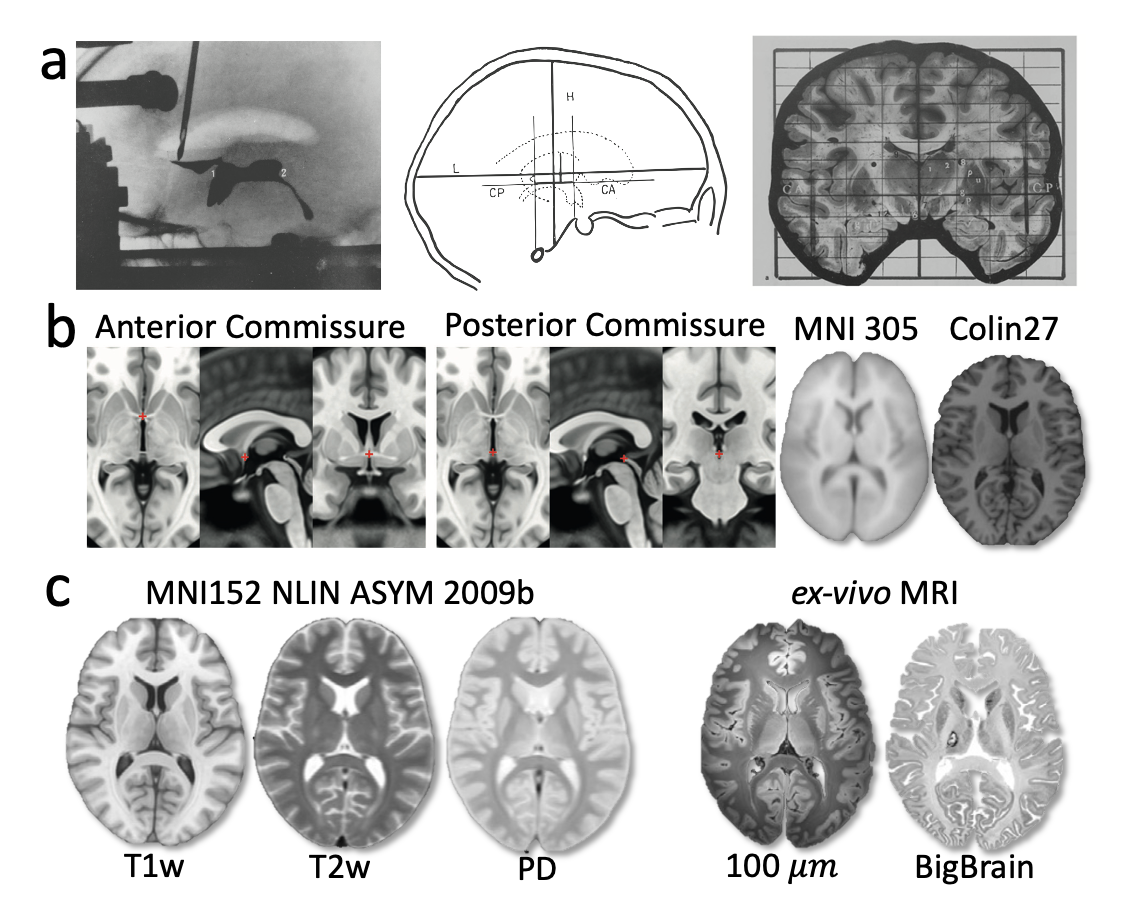
\includegraphics[width=0.85\linewidth]{figs/ch1_Figure_templates.png}
    \caption{Emergence of Stereotactic Spaces. (a) Classical Talairach space defined by stereotactic landmarks \cite{Talairach1957-eb}. (b) Early MRI-based average brain created in Talairach space \cite{Collins1994-dx}. (c) Modern templates \cite{Fonov2011-ck,Edlow2020-mo, Amunts2013-vu} improved using nonlinear registration.}
    \label{fig:ch1_Figure_templates}
\end{figure}

These early innovations established the foundation for population-based brain templates that emerged with the advent of MRI (see Section~\ref{sec:MRI}). The Montreal Neurological Institute (MNI) developed average brain templates derived from multiple individuals, enabling more representative spatial normalization across subjects. An important example is the MNI305 template \cite{Collins1994-ue}, which leveraged manually defined stereotactic landmarks (i.e., AC and PC) to align MRI scans of 305 individuals, approximating the Talairach space. This marked a convergence between classical stereotactic principles and neuroimaging, allowing more representative spatial normalization between subjects (Figure \ref{fig:ch1_Figure_templates}b). Since then, further improvements in nonlinear image registration (see Section~\ref{sec:registration}) have culminated in brain templates \cite{Fonov2009-oi} that preserve anatomical detail and support more accurate inter-subject alignment (Figure \ref{fig:ch1_Figure_templates}c).

Today, stereotactic spaces underpin a wide range of neuroimaging applications, from structural and functional mapping to large-scale meta-analyses \cite{Yarkoni2011-sr,Dockes2020-nw}. These frameworks facilitated the development of shared databases that encompass anatomical, cytoarchitectonic, and functional information \cite{Eickhoff2005-qb}. Despite advances in non-invasive neuroimaging and image registration, fundamental stereotactic principles remain central to both neurosurgical navigation and brain mapping.

\subsection{Deep Brain Stimulation}
Deep brain stimulation (DBS) is a stereotactic procedure that involves the targeted implantation of electrodes into deep brain nuclei to modulate dysfunctional neural circuits. Since its formal introduction by Alim Benabid in the late 1980s \cite{Benabid1987-mp}, DBS has revolutionized the management of various neurological disorders by providing a reversible, adjustable, and less destructive alternative to lesion-based surgeries \cite{Limousin1990-oz,The-Deep-Brain-Stimulation-for-Parkinson-s-Disease-Study-Group2001-ss}. To date, DBS has been implanted in over 250,000 patients worldwide \cite{Schulder2023-aj}, primarily for the treatment of movement disorders such as Parkinson's disease (PD), essential tremor, dystonia, and Tourette’s syndrome, as well as for select psychiatric conditions including obsessive-compulsive disorder and treatment-resistant depression \cite{Lozano2019-dv}.

The subthalamic nucleus (STN) is the most commonly targeted structure in DBS for PD \cite{Lozano2019-dv}. This lens-shaped nucleus (Figure \ref{fig:ch1_Figure_whymm}, roughly 10 mm in length, is located inferior to the thalamus, adjacent to the substantia nigra and lateral to the red nucleus (RN) \cite{Prasad2024-hi}. The STN acts as a major relay within the basal ganglia (BG) \cite{DeLong2007-cv}. It receives convergent cortical, pallidal, and thalamic inputs and is involved in regulating motor output within the BG circuit \cite{DeLong2007-cv,Jeon2022-wg}. Due to its integrative role, DBS of the STN results in significant motor improvements \cite{Hermann2024-tr}-but also in unwanted side effects if adjacent fiber tracts or nearby structures are inadvertently activated \cite{Kiss2007-mu,Reich2022-jf}.

Despite widespread clinical use, the therapeutic mechanisms of DBS remain poorly understood. Initial theories proposed a “functional lesion” effect, where high-frequency stimulation inhibits overactive neurons locally \cite{Benabid1987-mp, Benabid1996-jd}. DBS can also be viewed as a network-level modulator, capable of reshaping oscillatory activity and restoring information flow across distributed brain networks \cite{Miocinovic2013-rs,Herrington2016-xr}. The therapeutic effects vary by condition and symptom: tremor may improve within seconds, whereas benefits in dystonia or depression can take weeks to months, suggesting additional contributions from synaptic plasticity and long-term network reorganization \cite{Ashkan2017-hb}. These insights support an expanded view of DBS as a dynamic intervention capable of reshaping dysfunctional brain circuits over multiple timescales.

\subsection{Why millimeters matter}
\label{sec:whymm}
Achieving therapeutic benefit from DBS requires the millimetric implantation of electrodes. While stereotactic neurosurgery has embraced the need for accuracy, DBS uniquely amplifies this demand due to three converging factors: (1) the small size of target structures, (2) their complex anatomical context, and (3) the highly localized nature of stimulation effects.

DBS targets such as the STN, globus pallidus internus, and ventral intermediate nucleus are a few millimeters in size. Within these already small structures, stimulation is often directed at even smaller subregions that are functionally specialized. In the case of the STN, for example, different functional subzones are associated with distinct symptom domains, ranging from motor control to mood and behavior \cite{Hollunder2024-wc}. Hence, the STN is a DBS target for a range of neurological and psychiatric conditions, including PD \cite{Deuschl2006-ar}, dystonia \cite{Ostrem2017-rw}, Tourette’s syndrome \cite{Mallet2008-ky}, and obsessive-compulsive disorder \cite{Dai2022-uy}. These therapeutic zones are in close proximity to each other, so even a 1-2 mm deviation in electrode placement can shift stimulation to less effective or potentially adverse area \cite{Akram2017-ru}.

DBS targets are located within an anatomically crowded and heterogeneous environment. The subcortex is traversed by multiple orthogonal and intersecting fiber tracts, with neighboring structures often fulfilling opposing or unrelated functions. For example, the internal capsule lies adjacent to the STN and carries motor fibers from the cortex; inadvertent stimulation here can cause contractions or dysarthria \cite{Tripoliti2011-ca}. Similarly, stimulation that extends into associative or limbic territories of the STN may alter cognition or emotion \cite{Mallet2007-ur}.

\begin{figure}[hbt!]
    \centering
    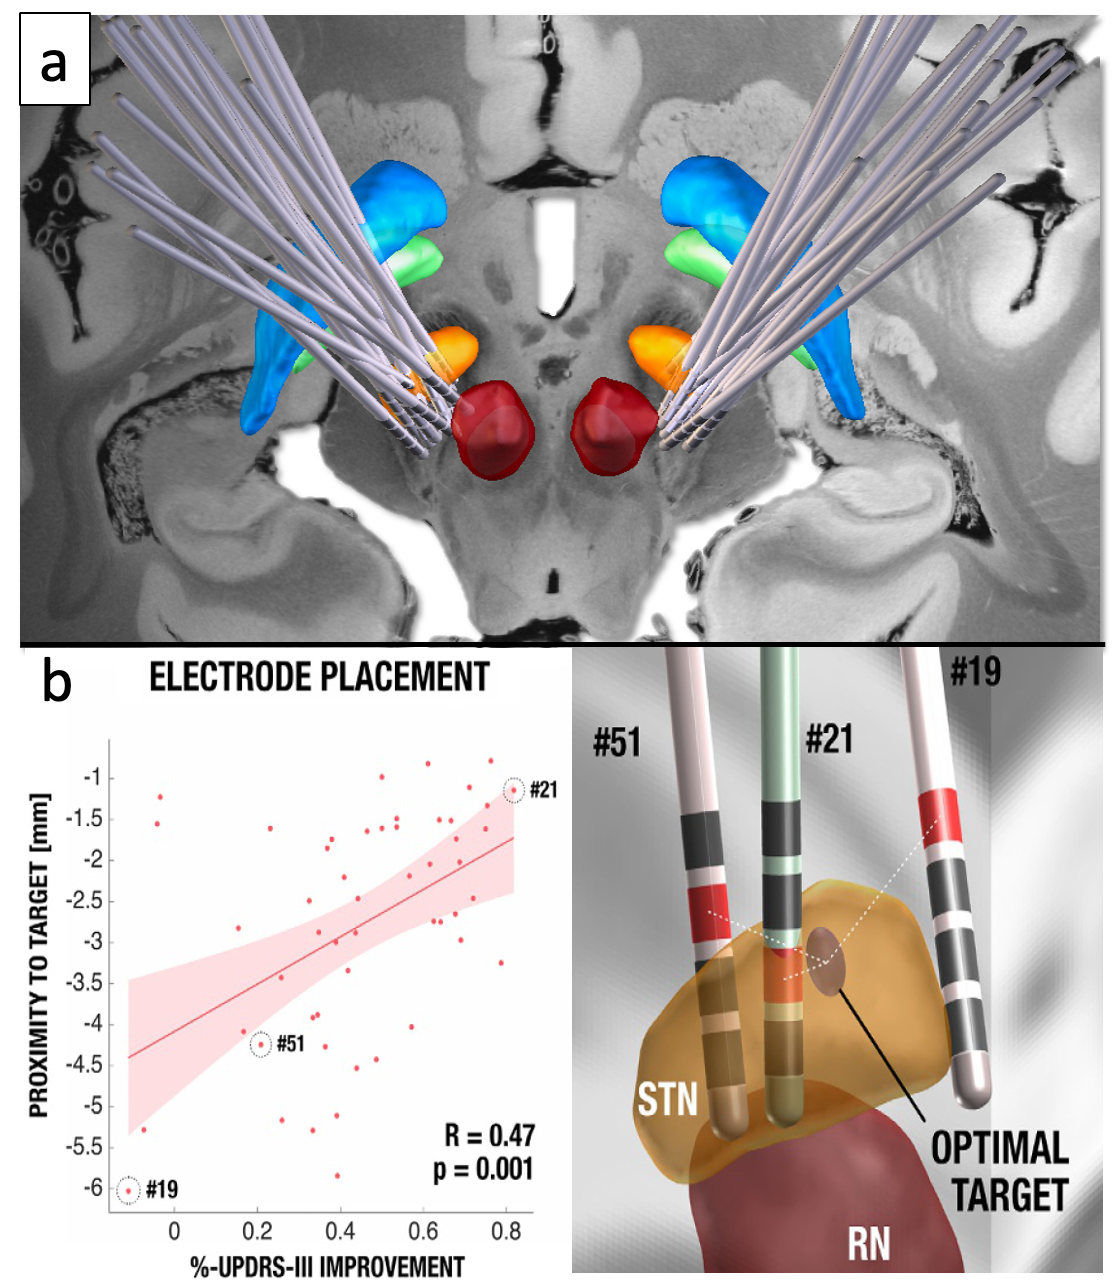
\includegraphics[width=1\linewidth]{figs/ch1_Figure_whymm.png}
    \caption{Why millimeters matter in deep brain stimulation (DBS). (a) Example from a population study showing DBS electrodes warped to a common atlas. (b) Correlation between electrode location and clinical outcome, illustrating how a difference of 2~mm (between patients \#51 and \#21) could correspond to a 60\% difference in therapeutic response. Figure in panel b is modified from an open-access article by \cite{Horn2018-qq}}
    \label{fig:ch1_Figure_whymm}
\end{figure}

Unlike systemic therapies, DBS exerts its effect over a localized volume of tissue, typically within a 1–3 mm radius of the electrode. The “volume of tissue activated” (VTA) depends on factors like stimulation amplitude, pulse width, impedance, and local tissue conductivity \cite{McIntyre2006-wh,Butson2007-bn}. This physical limitation means that even a precisely shaped VTA may fail to engage the intended neural circuits if the electrode is off target. Empirical studies show dramatic differences in clinical outcomes between patients with electrodes separated by as little as 2 mm (Figure \ref{fig:ch1_Figure_whymm}b), underscoring the high spatial gradient of therapeutic response \cite{Horn2018-qq, Maks2009-ci}. Thus, this spatial demand determines the threshold for side effects, stimulation battery usage, and the degree of parameter programming required postoperatively. 

From a surgical standpoint, millimetric accuracy is essential not only for localizing the target but also throughout the DBS electrode implantation process. DBS electrodes may traverse up to 80–100 mm of brain tissue, depending on the entry point and target. Deviations in trajectory may increase the risk of complications such as hemorrhage or unintended tissue damage \cite{Ben-Haim2009-os,Rajabian2023-st}. Maintaining millimetric control over the surgical path is therefore critical to ensuring safe DBS electrode implantation.
 
In summary, the clinical success of DBS hinges on achieving and validating millimetric precision. This imperative has driven the evolution of stereotactic techniques, neuroimaging protocols, and computational tools, all aimed at minimizing spatial error. As such, the millimetric demands of DBS serve as a central challenge and benchmark for any system designed to support neurosurgical targeting.

\section{Magnetic Resonance Imaging}
\label{sec:MRI}
MRI origins trace back to the discovery of nuclear magnetic resonance (NMR) by Felix Bloch and Edward Purcell in 1946, who independently demonstrated that atomic nuclei emit measurable radiofrequency (RF) signals when placed in a magnetic field \cite{Bloch1946-ob, Purcell1946-jd}. Subsequent advances, including the development of pulsed NMR by Ernst \cite{Ernst1990-we} and the proposal of spatial encoding through magnetic field gradients by Ernst and Anderson \cite{Ernst1966-yx}, laid the foundation for imaging applications. In the early 1970s, Paul Lauterbur and Peter Mansfield independently introduced the concepts of spatially resolved magnetic resonance imaging, establishing the principles that would revolutionize biomedical imaging \cite{Lauterbur1973-wf,Mansfield1977-ru}. 

Today, MRI is the diagnostic modality of choice for soft tissue visualization and is routinely used in neurosurgical planning, including DBS. Its flexibility, safety, and ability to generate diverse tissue contrasts have made it indispensable for anatomical localization and trajectory planning. In this section, we first review the key physical principles underlying MRI, then examine specialized MRI techniques employed during DBS, and finally highlight the challenges that limit the effectiveness of MRI in subcortical structure visualization.

\subsection{MRI Physics Fundamentals}

MRI is based on the principles of NMR, where atomic nuclei with non-zero spin, primarily hydrogen protons in biological tissues, absorb and re-emit RF energy when placed in a strong magnetic field. In a static magnetic field \(B_0\), proton spins precess at the Larmor frequency:
\begin{equation}
\omega_0 = \gamma B_0
\end{equation}
where \( \omega_0 \) is the precessional (angular) frequency and \( \gamma \) is the gyromagnetic ratio (approximately 42.58 MHz/T for hydrogen). By transmitting a radiofrequency (RF) pulse at this resonant frequency (the $B_1$ field perpendicular to $B_0$), the net magnetization $M$ of proton spins can be tipped away from alignment with $B_0$, producing a detectable MR signal as the spins precess and relax back to equilibrium. This excitation and subsequent signal emission is the essence of NMR and forms the basis of MRI signal generation.

After excitation, the perturbed spins return to equilibrium through two independent relaxation processes characterized by time constants $T_1$ and $T_2$. The longitudinal relaxation (spin-lattice relaxation) with time constant T1 describes the recovery of the $M_z$ component (along the $B_0$ axis) toward its equilibrium value. The transverse relaxation (spin-spin relaxation) with time constant T2 describes the decay of the $M_{xy}$ component (perpendicular to $B_0$) due to dephasing of spins. Quantitatively, one may write the solutions of the Bloch equations for recovery and decay as:
\begin{itemize}
    \item \textbf{Longitudinal relaxation time} (\(T_1\)): Describes the recovery of the longitudinal component of magnetization, \(M_z\), as it realigns with the static magnetic field \(B_0\) following excitation. The time course of this recovery is governed by:
    \begin{equation}
    M_z(t) = M_0 \left(1 - e^{-t/T_1}\right)
    \end{equation}
    Here, \( M_0 \) represents the equilibrium magnetization—i.e., the maximum net magnetization achievable along the longitudinal axis in thermal equilibrium. It is determined by the strength of the external field \(B_0\), the spin density of the tissue, temperature, and the gyromagnetic ratio. Immediately after RF excitation, \(M_z = 0\), and over time, it asymptotically returns to \(M_0\).

    \item \textbf{Transverse relaxation time} (\(T_2\)): Describes the decay of the transverse magnetization component, \(M_{xy}\), which is created when the net magnetization vector is tipped into the transverse (x-y) plane by an RF pulse. This decay arises from the dephasing of individual proton spins due to local magnetic field inhomogeneities:
    \begin{equation}
    M_{xy}(t) = M_{xy}(0) \, e^{-t/T_2}
    \end{equation}
    The term \( M_{xy}(0) \) denotes the initial transverse magnetization at time \( t = 0 \), immediately after RF excitation. It reflects the full coherence of spins in the transverse plane and is directly proportional to the strength of the induced MR signal. Over time, dephasing interactions cause a loss of this coherence, leading to exponential signal decay characterized by the tissue-dependent constant \(T_2\).
\end{itemize}

Each tissue has characteristic $T_1$ and $T_2$ values, so by timing the signal readout appropriately MRI can weight the image contrast by these differences. For example, fat tissue has a short $T_1$ (bright on T1-weighted images) whereas cerebrospinal fluid has a long $T_1$ (dark on T1-weighted images); similarly, fluid has a long $T_2$ (bright on T2-weighted images) while white matter has a shorter $T_2$. These relaxation properties underlie the rich soft-tissue contrast of MRI, enabling clear differentiation of structures based on their composition and environment. 

To form an image from the NMR signal, MRI employs spatial encoding using magnetic field gradients. Three orthogonal gradient coils apply slight spatial variations to the magnetic field ($B_x$, $B_y$, $B_z$), allowing location-specific modulation of the Larmor frequency and phase. A slice-selection gradient combined with a frequency-selective RF pulse excites a thin cross-sectional slice of tissue. After excitation, frequency-encoding (readout) gradients impose position-dependent frequency shifts along one axis, while phase-encoding gradients impart position-dependent phase shifts along the orthogonal in-plane axis. The resulting signals from the receiver coil are stored as samples in k-space, an array representing spatial frequency information. The complete k-space data is then mathematically transformed (via the inverse Fourier transform) to reconstruct the spatial image.

\subsection{Multimodal MRI and Sequence Design}
A single MRI contrast is often insufficient to optimally visualize all relevant structures for DBS targeting \cite{Boutet2021-vg,Treu2020-ih}. Modern DBS planning therefore leverages multiple MRI sequences (i.e., multimodal MRI) to improve anatomical localization and targeting accuracy (Figure \ref{fig:ch1_Figure_STN_MRI}). Below we enumerate various MRI modalities and their contributions to DBS targeting.

\begin{figure}[hbt!]
    \centering
    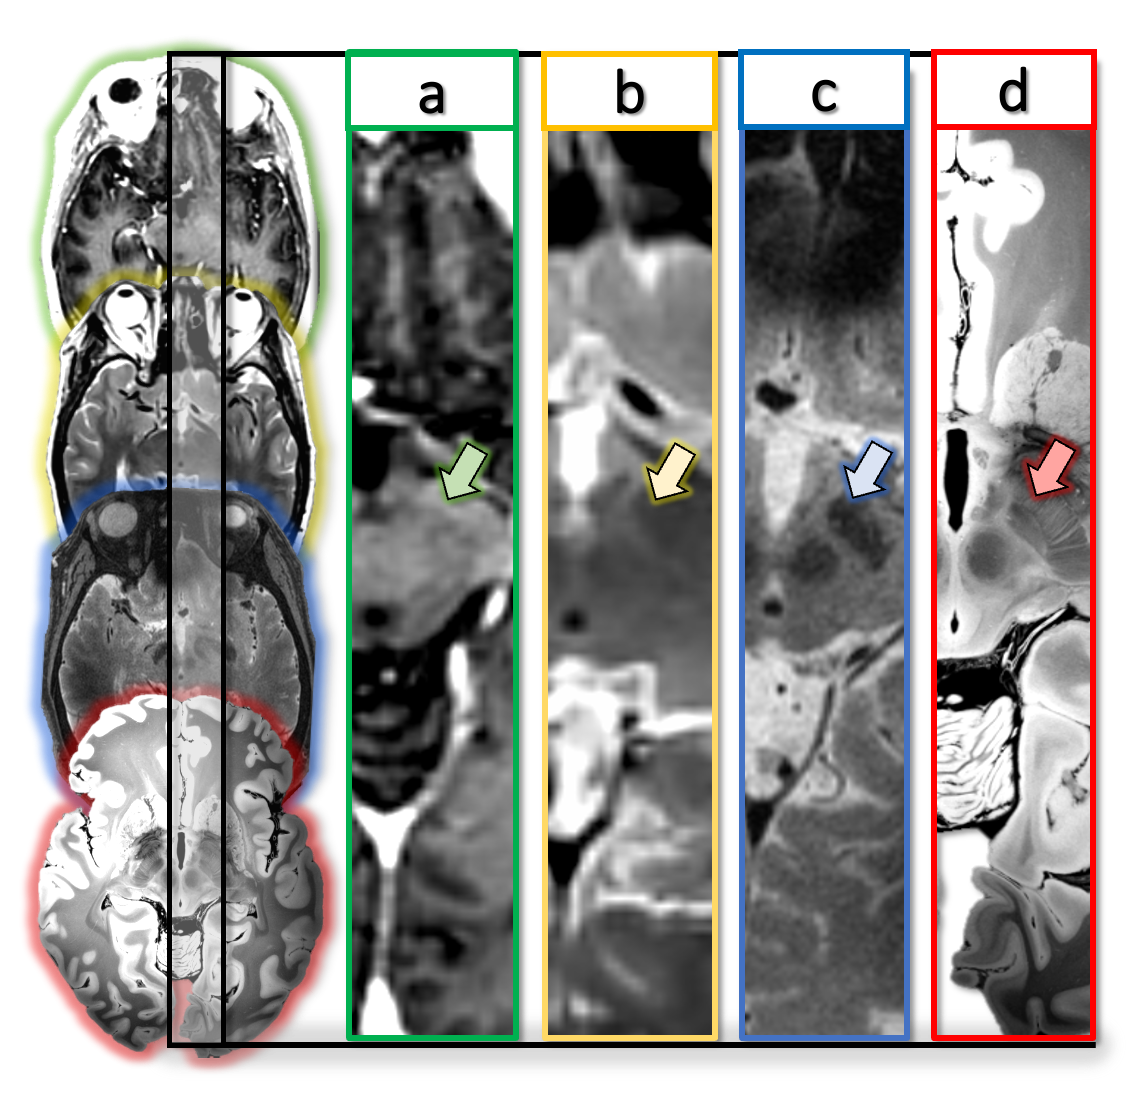
\includegraphics[width=1\linewidth]{figs/ch1_Figure_STN_MRI.png}
    \caption{
    Visualization of the subthalamic nucleus (STN) across different MRI modalities. (a) Clinically acquired T1-weighted MRI (MP2RAGE) at 1.5 Tesla with gadolinium contrast, enhancing visualization of blood vessels. (b) T2-weighted MRI acquired from the same subject and scanner as in (a). (c) High-resolution T2-weighted MRI (SPACE sequence) acquired at 7 Tesla. (d) \textit{ex vivo} MRI acquired at 7 Tesla for comparison \cite{Edlow2020-mo}. The STN is indicated by colour-mapped labels.}
    \label{fig:ch1_Figure_STN_MRI}
\end{figure}

\textbf{T1-weighted MRI (T1w):} T1-weighted sequences, such as Magnetization-Prepared RApid Gradient Echo (MPRAGE), provide a detailed anatomical overview with high gray-white matter contrast \cite{Brant-Zawadzki1992-nw} and define important landmarks like the anterior and posterior commissures (AC-PC line). However, at clinical field strengths (i.e., 1.5 or 3 Tesla (T)), conventional T1w imaging offers limited contrast between deep gray matter structures themselves. For instance, the STN is poorly distinguished on standard T1w images.

\textbf{T2-weighted and FLAIR MRI (T2w/FLAIR):} T2-weighted sequences highlight water content and offer improved contrast for visualizing deep brain structures. T2w images depict the STN as a hypointense (dark) almond-shaped region distinguishable from surrounding BG anatomy. T2-FLAIR (fluid-attenuated inversion recovery) sequences suppress cerebrospinal fluid signals and enhance contrast at tissue interfaces, facilitating delineation of boundaries within the thalamus and pallidum. While direct comparisons between FLAIR and other imaging modalities remain limited \cite{Boutet2021-vg}, a 3T FLAIR sequence employing sampling perfection with application-optimized contrasts by using different flip angle evolution (SPACE) for preoperative targeting resulted in reduced geometric distortion and improved contrast with surrounding anatomy. Notably, this approach was associated with superior clinical outcomes at 12-month follow-up compared to conventional T2w imaging \cite{Senova2016-bh}.

\textbf{Inversion-Recovery MRI (FGATIR):}  
Fast Gray Matter Acquisition T1 Inversion Recovery (FGATIR) is a specialized MRI sequence designed to improve the visualization of deep gray matter structures for DBS targeting. Unlike conventional T1w or T2w scans, FGATIR employs a full 180° inversion pulse with a short inversion time to selectively nullify white matter signal, thereby enhancing contrast at the interface between gray and white matter. This feature is particularly useful in DBS planning, as many targets are embedded within heavily myelinated fiber tracts. A pilot study demonstrated that FGATIR provided clearer visualization of structures such as the internal medullary lamina of the GPi, the STN/substantia nigra interface, and fiber bundles from the internal capsule piercing the striatum-features not consistently resolved on other sequences \cite{Sudhyadhom2009-xx}. Quantitatively, FGATIR produced higher contrast-to-noise ratios (CNRs) across multiple regions of interest. For example, the CNR at the STN and substantia nigra was more than threefold higher on FGATIR compared to T2-FLAIR, facilitating better localization of the STN's inferior boundary. Overall, FGATIR offers a promising balance between contrast, resolution, and acquisition time for DBS planning, and has been increasingly adopted as a core component of multimodal MRI protocols for subcortical targeting \cite{Neudorfer2022-nj}.


\textbf{Susceptibility-Weighted Imaging and Quantitative Susceptibility Mapping (QSM):} MRI sequences sensitive to magnetic susceptibility-including T2*-weighted imaging, phase imaging, and QSM-exploit the iron content of deep brain nuclei. Structures like the STN are iron-rich and produce local magnetic field inhomogeneities detectable by these techniques. QSM, in particular, generates quantitative maps of magnetic susceptibility and provides superior contrast-to-noise ratios compared to conventional T2*-weighted imaging. This improved depiction facilitates more reliable boundary identification of small targets like the STN \cite{Liu2013-zm}, substantia nigra \cite{Chen2021-tj}, and zona incerta (ZI) \cite{Lau2020-dh} . Although susceptibility imaging is prone to artifacts-such as blooming distortions near air-tissue interfaces-QSM algorithms mitigate these effects by deconvolving the field perturbations, yielding more accurate anatomical localization.

\textbf{Diffusion-Weighted Imaging (DWI) and Tractography:} While conventional MRI depicts structural anatomy, diffusion MRI captures information about white matter pathways. Diffusion Tensor Imaging (DTI) and tractography methods can reconstruct fiber tracts that emanate from or pass near DBS targets \cite{Rodrigues2018-jt}. In clinical practice, tractography has supported a shift toward connectomic targeting, where stimulation is guided not solely by anatomy but also by network connectivity \cite{Horn2020-wf}. For example, tractography enables visualization of the corticospinal tract to avoid during Vim targeting for tremor, or the motor versus limbic subdivisions of the STN for tailored therapy \cite{Calabrese2016-xi}. Although DTI-based tractography lacks direct histological validation and is sensitive to distortions, it remains the only non-invasive method to visualize patient-specific brain networks \cite{Coenen2016-pd}, and is increasingly incorporated into DBS planning to optimize both therapeutic efficacy and side effect profiles.

By integrating these complementary MRI modalities, modern DBS planning protocols enhance the visualization of deep brain structures and fiber pathways. Although most DBS workflows use T1w imaging for stereotactic referencing (e.g., AC-PC annotation), all the other modalities are seldom used concurrently. Instead, DBS centers acquire one or two additional modalities depending on the target. This multimodal synergy reduced the reliance on indirect atlas-based approximations and exploratory microelectrode recordings. As a result, MRI-guided DBS has improved targeting precision, reduced operative times, and expanded the scope of treatable disorders through anatomically and network-informed strategies.

\subsection{Ultra-High Field MRI}
\label{sec:uhf_mri_physics}

Ultra-high field (UHF) MRI, defined as systems operating at magnetic field strengths of 7T or higher, offers significant advantages in neuroimaging due to fundamental physical improvements in signal acquisition. These gains directly translate into enhanced visualization of deep brain structures relevant to DBS targeting.

The signal-to-noise ratio (SNR) in MRI increases approximately linearly with magnetic field strength, with 7T MRI offering a 2--3-fold improvement over 3T systems \cite{Trampel2019-fa}. This gain in SNR can be traded for higher spatial resolution, which is particularly advantageous for DBS planning. For example, 7T MRI enables the acquisition of isotropic voxels as small as 0.5~mm, improving the delineation of small deep brain structures and their subregions. This benefit can be illustrated using the STN, a common DBS target with an estimated volume of 240~mm\textsuperscript{3} and a maximal extent of approximately 10~mm. At standard clinical resolution (1~mm isotropic), the STN is represented by roughly 240 voxels, with only 10 voxels spanning its longest axis. Each voxel encompasses an estimated 2300--2400 neurons \cite{Hamani2004-zr,Hardman2002-ru}, reducing anatomical specificity. Increasing spatial resolution to 0.5~mm isotropic increases the total voxel count to approximately 1920, with about 20 voxels along the nucleus’s longest dimension. At this finer scale, each voxel represents around 300 neurons, significantly enhancing anatomical fidelity and reducing partial volume effects.

Tissue relaxation properties undergo significant changes that enhance MRI contrast between different brain structures at 7T. Specifically, T1 relaxation times increase, and T2* relaxation times decrease, leading to improved differentiation between gray and white matter. This enhanced contrast is particularly beneficial for visualizing small and previously elusive deep brain nuclei, which are critical targets in DBS procedures. One notable example is the zona incerta (ZI), a small gray matter region situated in the subthalamic area. Historically, the ZI has been challenging to visualize in vivo due to its size and location. However, recent advancements have demonstrated that high-resolution T1 mapping at 7T allows for robust visualization of the ZI and its surrounding white matter structures along the entire rostrocaudal axis. This capability enables comprehensive anatomical characterization of this previously obscure deep brain region, facilitating more accurate DBS targeting \cite{Lau2020-dh}. Similarly, the delineation of intra-thalamic nuclei has been significantly improved at 7T. By adjusting inversion times to null white matter signals, enhanced contrast between thalamic nuclei can enable their reliable identification and segmentation. This advancement holds promise for refining DBS targeting strategies, particularly for conditions like essential tremor, where DBS is targeting specific thalamic nuclei \cite{Tourdias2014-un}.

Moreover, as shown in a comparative imaging study by Forstmann and colleagues, even when 3T images are highly optimized, they fail to match the clarity, boundary sharpness, and contrast seen in 7T acquisitions. For example, the STN and globus pallidus demonstrate significantly sharper lateral and posterior borders at 7T under T2*-weighted protocols. Additionally, the ventral intermediate nucleus (VIM) of the thalamus-difficult to delineate directly at any field strength-becomes more reliably identified through the improved contrast of neighboring thalamic nuclei at 7T \cite{Forstmann2017-gz}. Furthermore, a comparative outcome study by Middlebrooks and colleagues directly assessed patients undergoing DBS for essential tremor planned using either 3T or 7T MRI. Patients in the 7T cohort experienced significantly greater tremor reduction and required lower stimulation currents. Although the average electrode positions were comparable, the 7T cohort demonstrated significantly lower variance in the final location of the electrode, underscoring higher targeting precision during DBS \cite{Middlebrooks2024-gb}.

UHF MRI has advanced the visualization of deep brain structures, offering unprecedented contrast and resolution that enhance DBS targeting \cite{Isaacs2020-gq}. However, its integration into clinical workflows remains limited by both technical and logistical constraints. First, susceptibility artifacts-exacerbated at air-tissue interfaces near the skull base-can impair signal fidelity in regions adjacent to common DBS targets. Second, increased \(B_0\) and \(B_1\) field inhomogeneities at 7T introduce signal dropouts and nonuniform contrast, complicating the interpretation of small, deep nuclei \cite{Okada2022-fg}. Additionally, the higher specific absorption rate (SAR) at ultra-high field strengths may restrict sequence design and limit the use of certain clinically useful protocols, such as long echo-train or spin-echo–based acquisitions \cite{Okada2022-ln}. Spatial distortions-driven by both system-related nonlinearity and patient-specific susceptibility effects-can result in displacements of up to 2 mm near midbrain targets \cite{Kirby2023-la}, and distortion correction algorithms may introduce secondary errors if improperly applied. Beyond these imaging-specific limitations, widespread clinical adoption is also hindered by the limited availability of 7T systems globally, as they remain concentrated in research centers and require specialized infrastructure, coils, and workflows \cite{Forstmann2017-gz,Boutet2021-vg}. These challenges underscore a need for hybrid imaging and prepossessing strategies, alongside workflow standardization during DBS.

\subsection{Limitations of MRI in DBS Targeting}
\label{sec:MRI_limitations}

Despite significant advancements in MRI technology, several critical limitations hinder its optimal application in stereotactic planning for DBS. These challenges can be broadly categorized into issues related to sequence validation, anatomical generalizability, geometric fidelity, and clinical implementation.

\textbf{Lack of Standardization and Outcome-Linked Validation:} There is limited consensus on the most appropriate MRI sequences to directly visualize common DBS targets \cite{Vitek2010-cn,Middlebrooks2020-vv}. Although specialized sequences such as FGATIR and QSM have demonstrated improved visualization, few studies have rigorously compared these sequences or established their superiority in improving clinical outcomes compared to traditional indirect targeting methods \cite{Boutet2021-vg}. The lack of prospective validation and a unified protocol for DBS targeting remains a major gap in the literature.

\textbf{Limited Generalizability to Clinical Populations:}
Many MRI optimization studies have been conducted in healthy volunteers rather than the patient populations typically considered for DBS \cite{Boutet2021-vg}. These patients often exhibit disease-related and age-related brain atrophy, including reduced white matter volume \cite{Bonneville2005-vl,Lee2011-rf}, which can significantly affect the visibility of deep brain structures. As a result, sequences validated in healthy cohorts may underperform in clinical settings.

\textbf{Geometric Distortion and Registration Error:}
High-resolution MRI sequences-especially those using gradient-echo-based mechanisms (e.g., SWI, QSM)-are prone to geometric distortions arising from magnetic susceptibility effects. These distortions can compromise the spatial fidelity required for stereotactic neurosurgery, where errors of 1--2~mm can have significant clinical consequences \cite{Boutet2021-vg, Rasouli2018-sn, Lau2018-fp}. Furthermore, quantitative sequences (e.g., QSM) optimized for target visualization often fail to adequately depict anatomical landmarks or fiducials used in surgical navigation (e.g., AC and PC), necessitating registration to anatomical MRI or CT dataset. The accuracy of such registration pipelines is poorly quantified, and errors introduced in this step may accumulate and degrade targeting accuracy.

\textbf{Practical Constraints and Hardware Incompatibility:}
The implementation of advanced MRI sequences is often constrained by hardware limitations. For example, head coils that offer superior signal-to-noise ratios may not physically accommodate stereotactic head frames used in surgical planning \cite{Boutet2021-vg}. Similarly, while UHF MRI provides enhanced spatial resolution and contrast, it is currently incompatible with most commercial stereotactic systems and requires additional processing. Consequently, UHF images must be coregistered with stereotactic imaging from another modality (e.g., CT), a step that may introduce additional errors \cite{Lenglet2012-ii}.

\textbf{Experimental Status of Connectomic Techniques:}
Emerging techniques such as functional MRI and DWI tractography are beginning to reshape DBS targeting strategies by shifting focus from discrete anatomical nuclei to distributed structural and functional networks. Although retrospective studies suggest that connectomic targeting correlates with clinical response, these techniques remain largely experimental. Their clinical adoption is limited by a lack of prospective validation and the complexity of postprocessing pipelines \cite{Horn2017-bi}.

Thus, while MRI has greatly enhanced DBS targeting, it does not fully eliminate the need for complementary strategies such as multimodal imaging, atlas integration, and image registration pipelines to achieve the precision required for optimal outcomes. These solutions are further explored in the sections that follow.

\section{Image Registration}
\label{sec:registration}
Image registration is a fundamental step in neuroimaging analysis, facilitating spatial alignment of imaging volumes over time and modalities (e.g., MRI and CT) or to stereotactic spaces such as the MNI space \cite{Risholm2011-rm}. In DBS, registration plays a critical role in maintaining spatial continuity throughout the surgical workflow \cite{Geevarghese2016-qo}. Accurate coregistration ensures that anatomical information derived from preoperative MRI can be reliably transferred to stereotactic planning coordinates and subsequently reconciled with postoperative imaging for reliable DBS electrode localization and verification \cite{Lofredi2022-wi,Abbass2025-el}.

\subsection{Image Registration Fundamentals}
In its most general form, image registration aims to estimate a transformation \( v: \Omega_T \rightarrow \Omega_S \) that maps coordinates from the fixed image domain \( \Omega_T \) to the moving image domain \( \Omega_S \), such that the transformed moving image \( \tilde{S}(x) = S(v(x)) \) becomes aligned with the fixed image \( T(x) \). This process is commonly formulated as the following optimization problem:
\begin{equation}
    \arg\min_{v} \, \mathcal{C}(S \circ v, T) + \lambda \, \mathcal{R}(v)
    \label{eq:registration_loss}
\end{equation}

where \( \mathcal{C}(S \circ v, T) \) is a similarity metric that quantifies the alignment between the transformed moving image and the fixed image, \( \mathcal{R}(v) \) is a regularization term that encourages smoothness or anatomical plausibility of the transformation, and \( \lambda \) is a weighting parameter that balances data fidelity with regularization.

\paragraph{Transformation Models.}
Registration transformations are typically categorized based on their degrees of freedom (DoF), which determine how flexibly one image can be mapped to another \cite{Chen2023-wx, Zitova2003-ds, Maintz1998-gs}.

\begin{itemize}
    \item \textbf{Rigid} transformations preserve distances and angles by allowing only translation and rotation (6 DoF).
    
    \item \textbf{Affine} transformations extend rigid transformations by incorporating scaling and shearing (12 DoF), enabling global shape changes while preserving collinearity and parallelism.
\end{itemize}

Both rigid and affine transformations can be expressed in matrix form as:
\begin{equation}
    v(x) = \mathbf{M}x + t
    \label{eq:affine}
\end{equation}
where \( \mathbf{M} \in \mathbb{R}^{3 \times 3} \) encodes linear transformations (rotation, scaling, shear), and \( t \in \mathbb{R}^3 \) is a translation vector. 

These transformation models are computationally efficient and commonly used for intra-subject alignment across imaging sessions or modalities, where the underlying anatomy remains relatively unchanged \cite{Jenkinson2002-ab}. However, their global nature limits their ability to capture localized anatomical differences, which is particularly important in populations with neurodegeneration, lesions, tumors, or developmental abnormalities. Consequently, rigid and affine transformations are frequently employed as initialization steps for more flexible, nonlinear registration approaches.
\begin{itemize}
\item \textbf{Nonlinear (Deformable)} transformations introduce spatially varying displacements to capture local anatomical variation:
\begin{equation}
    v(x) = x + u(x)
    \label{eq:deformable}
\end{equation}
\end{itemize}
where \( u(x) \) is a dense smooth displacement field defined in the image domain. 

These transformations can accommodate complex inter-subject differences and are essential for high-precision applications such as brain morphometry, longitudinal studies, and label propagation from atlases. The most commonly used implementation diffeomorphic frameworks such as Symmetric Normalization (SyN) \cite{Avants2008-ek, Beg2005-yo}.

\paragraph{Similarity Metrics.}
To quantify alignment quality between the fixed image \( T(x) \) and the transformed moving image \( \tilde{S}(x) \), similarity metrics assess how well image intensities correspond after transformation. The choice of metric depends on the imaging modality and underlying intensity relationships:

\begin{itemize}
    \item \textbf{Sum of Squared Differences (SSD)} is a simple intensity-based metric suitable for \textit{intra-modality} registration, where images share similar intensity profiles. It assumes a linear relationship between corresponding intensities and penalizes squared voxel-wise differences:
    \begin{equation}
        \mathcal{C}_{\text{SSD}}(T, \tilde{S}) = \sum_{x \in \Omega_T} \left( T(x) - \tilde{S}(x) \right)^2
        \label{eq:ssd}
    \end{equation}
    SSD is computationally efficient but sensitive to noise and intensity non-uniformities~\cite{Zitova2003-ds,Maintz1998-gs}.

    \item \textbf{Normalized Cross-Correlation (NCC)} compares local intensity patterns and compensates for global intensity shifts or scaling. It is defined as:
    \begin{equation}
        \mathcal{C}_{\text{NCC}}(T, \tilde{S}) = \frac{\sum_x (T(x) - \mu_T)(\tilde{S}(x) - \mu_{\tilde{S}})}{\|T - \mu_T\| \cdot \|\tilde{S} - \mu_{\tilde{S}}\|}
        \label{eq:ncc}
    \end{equation}
    where \( \mu_T \) and \( \mu_{\tilde{S}} \) are the mean intensities of the fixed and moving images, respectively. NCC is robust to linear intensity variations and is often used in rigid and affine intra-modality registration~\cite{Pluim2003-kb}.

    \item \textbf{Mutual Information (MI)} measures the statistical dependence between intensity values in multimodal images. It is defined as:
    \begin{equation}
        \mathcal{C}_{\text{MI}}(T, \tilde{S}) = - \left[ H(T) + H(\tilde{S}) - H(T, \tilde{S}) \right]
        \label{eq:mi}
    \end{equation}
    where \( H(\cdot) \) denotes Shannon entropy and \( H(T, \tilde{S}) \) is the joint entropy. MI is robust to modality differences and widely used in scenarios like MRI--CT registration~\cite{Maes1997-jb,Wells1996-at}.
\end{itemize}

\paragraph{Optimization and Regularization.}
Optimization strategies include multiresolution gradient descent, Powell methods, or stochastic algorithms, and are chosen based on the complexity of transformations and the metric used \cite{Song2017-kq}. Regularization terms \( \mathcal{R}(v) \) ensure that transformations are smooth and physically meaningful, especially in deformable registration, where large local variations could lead to anatomically implausible deformation warps \cite{Castano-Aguirre2024-db}.

\subsection{Brain Templates and Atlases}
\label{sec:template_atlas}
Early stereotactic neurosurgical procedures were guided by knowledge from cadaveric specimens and sections. Atlases such as those by Talairach and Tournoux \cite{Talairach1957-eb,Talairach1988-wk} or Schaltenbrand-Wahren \cite{Schaltenbrand1977-ge} provided sectional views of the brain with overlaid coordinate systems anchored to internal features like the AC and PC line. These atlases were designed to support proportional scaling, allowing neurosurgeons to infer the location of deep brain structures relative to patient anatomy using intraoperative imaging modalities such as ventriculography or angiography \cite{Conti2023-oo}. Through these frameworks, atlas-based targeting became a central feature of stereotactic planning.

The advent of digital neuroimaging transformed atlas-based targeting. With the introduction of MRI and CT, and later population-averaged anatomical datasets, the field shifted from fixed, printed atlases toward deformable, individualized imaging. This shift introduced a useful conceptual distinction: a \textbf{template} is now understood as a coordinate-defined brain volume-often an average of many individuals-that serves as a registration target for aligning individual images. Examples include the MNI templates \cite{Avants2008-ek,Fonov2009-oi}, which define modern stereotactic spaces.

An \textbf{atlas}, by contrast, is now commonly defined as an annotation or labeling schema superimposed onto a template \cite{Chakravarty2006-ln}. These can include deterministic labels (e.g., segmentations of the STN) or probabilistic maps reflecting anatomical variability. An example is the DBS Intrinsic Template AtLas (DISTAL), which is a subcortical atlas based on a multimodal, high definition MNI template series, histology and tractography \cite{Ewert2018-bn}. In practice, a subject's MRI is first registered to a template via nonlinear transformation; only then can atlas labels be transferred and interpreted in the subject's anatomical context.

Stereotactic spaces serve as common reference systems for aligning brain images, enabling comparisons between subjects and large-scale studies. This spatial standardization supported automated meta-analytic tools such as \texttt{NeuroSynth} \cite{Yarkoni2011-sr} and \texttt{NeuroQuery} \cite{Dockes2020-nw}, which aggregated reported coordinates from thousands of studies to identify consistent associations between brain and behavior. Stereotactic spaces allowed the neuroimaging community to build reproducible and interpretable models of the brain structure and function at the population level.

In DBS, stereotactic spaces serve two main goals: 1) during target localization and planning to visualize conspicuous targets \cite{Stancanello2006-vj} and 2) registration to a population-based template is employed by the majority of studies that attempt to understand stimulation effects on targeted neural circuits \cite{Neudorfer2023-wd}.

\subsection{Registration Tools and Pipelines}
Classical registration algorithms rely on similarity metrics (e.g., NCC or MI) and optimization strategies to estimate transformations that align a moving image to a fixed reference \cite{Hoffmann2024-yd}. Tools such as FMRIB's Linear Image Registration Tool (\texttt{FLIRT}) provide robust linear registration through affine transforms of six or twelve dof \cite{Jenkinson2001-bw, Jenkinson2002-ab}. However, to capture anatomical variability between individuals, nonlinear registration is typically required \cite{Klein2009-lv}. Tools such as FMRIB's Non-Linear Image Registration Tool (\texttt{FNIRT}; \cite{Jenkinson2001-bw}), Advanced Normalization Tools (\texttt{ANTs}; \cite{Avants2011-zs}) and Statistical Parametric Mapping (\texttt{SPM}; \cite{Ashburner2007-en}) implement deformable models that estimate dense and smooth displacement fields across the brain.

Comparative studies \cite{Klein2009-lv, Ewert2019-cc} previously evaluated the performance of various nonlinear deformation algorithms across more than 45,000 registrations. Their findings revealed that tools like \texttt{ANTs}, and SPM's Diffeomorphic Anatomical Registration using Exponentiated Lie algebra (DARTEL) consistently ranked highest in accuracy across multiple datasets and labeling protocols, underscoring their reliability in gross morphological alignment tasks.

Recent advances in deep learning (see Section~\ref{sec:deeplearning}) have introduced registration frameworks like \texttt{SynthMorph} \cite{Hoffmann2024-yd} and \texttt{EasyReg} \cite{Iglesias2023-ni}, which offer fast, anatomy-aware, and acquisition-agnostic affine and deformable registration. Both of \texttt{SynthMorph} and \texttt{EasyReg} are trained on synthetic data generated from label maps, enabling robust generalization across contrasts and resolutions. Unlike traditional methods that require manual tuning and preprocessing, deep learning driven registration performs joint affine-deformable registration without preprocessing, offering a reproducible, high-throughput alternative with state-of-the-art performance across diverse neuroimaging datasets. 

Modern preprocessing pipelines incorporate these tools into modular workflows. For instance, \texttt{fMRIPrep} is an analysis pipeline designed for robust anatomical and functional MRI preprocessing \cite{Esteban2019-oz}. It integrates tools from \texttt{ANTs}, \texttt{FreeSurfer} \cite{Fischl2012-dp}, \texttt{FSL}, and others to standardize preprocessing across diverse acquisition protocols while maximizing transparency via detailed quality reports. Although developed for functional MRI, its anatomical pipeline performs high-quality T1-to-template registration using \texttt{ANT's} symmetric diffeomorphic normalization (SyN) with careful bias correction and skull stripping. Similarly, \texttt{Lead-DBS} is a dedicated pipeline tailored for DBS imaging. It supports multispectral co-registration, subcortical-optimized normalization, and electrode reconstruction across clinical and research imaging environments. \texttt{Lead-DBS} incorporates nonlinear warping methods from \texttt{ANTs}, \texttt{SPM}, and \texttt{FSL}, and its registration performance has been evaluated across over 11,000 deformations for subcortical alignment. The validation paper \cite{Ewert2019-cc} demonstrated that multispectral normalization (e.g., using T1w and T2w images) improved the registration of DBS targets such as the STN and GPi to template space, yielding segmentation accuracies comparable to manual labels. 

In neurosurgical applications such as DBS, millimetric registration accuracy is critical. Thus, pipelines like \texttt{Lead-DBS} emphasize subcortical-focused normalization and brain-shift correction, and allow for visual inspection of co-registrations and electrode reconstructions \cite{Neudorfer2023-wd}. The increasing integration of registration pipelines with atlases and connectivity models has further enhanced their utility in DBS targeting, enabling patient-specific analyses anchored to standardized anatomical references.

\subsection{Limitations in Validation and Quality Control}
Despite its importance, image registration remains a major source of spatial error in neuroimaging pipelines \cite{Lau2019-eh, Abbass2022-lf}. The accuracy of registration can be influenced by various factors, including voxel size, contrast properties, presence of artifacts, and the choice of template or deformation model \cite{Klein2009-lv, Ewert2019-cc}. Yet, in practice, assessing the quality of a registration often depends on surrogate measures that may not always reflect true anatomical alignment.

Voxel overlap metrics such as the Dice or Jaccard coefficients remain widely used for evaluating registration performance. However, these measures are unitless and provide limited spatial quantification of alignment error. This lack of physical interpretability presents a significant limitation in neurosurgical contexts, where magnitude and directionality of spatial misalignment can impact clinical outcomes. Moreover, the dynamic range of voxel overlap metrics is relatively narrow—once a threshold of moderate overlap is achieved, these measures often saturate, making them insensitive to subtle but clinically meaningful misregistrations \cite{Lau2019-eh}. Beyond interpretability and dynamic range, the calculation of voxel overlap metrics requires accurate and reliable anatomical segmentations. Manual segmentation of brain structures is labor-intensive and requires expert anatomical knowledge. Automated segmentation methods, while efficient, may not always be trustworthy in cases of anatomical distortion, image noise, or low tissue contrast. These challenges collectively limit the utility of voxel overlap as a dependable measure for quality control in high-precision applications in neurosurgery.

Visual inspection remains the main mechanism for assessing registration quality in both research and clinical settings \cite{Neudorfer2023-wd,Esteban2019-oz}. However, this method is inherently subjective and may not reliably detect local or focal misregistrations, especially in deep brain regions with indistinct anatomical boundaries \cite{Bosma2024-cf,Rohlfing2012-kt}. Even experienced raters may overlook errors when differences are subtle or distributed across non-obvious regions of the image \cite{de-Senneville2020-am}. Furthermore, visual inspection of reformatted, subtraction, or variance images cannot always reliably distinguish accurate from inaccurate registrations \cite{Rohlfing2012-kt}. As a result, sole reliance on visual inspection risks underestimating the registration error, especially in an application like DBS where millimetric spatial correspondence is essential for optimal therapeutic benefit and minimizing side effects.

\section{Brain Coordinates} 
A fiducial, from 'fiducia' in Latin meaning trust or confidence, is a point of reference that marks a specific identifiable location in space. In neuroanatomy, a fiducial typically represents a reproducible anatomical feature, such as the AC or PC. These points serve as spatial anchors for assessing anatomical correspondence \cite{Schonecker2009-xj,Lau2019-eh} or describing and understanding the structure of the brain \cite{Abbass2022-lf}. The use of fiducials is rooted in classical stereotactic approaches, where the localization of deep brain structures depended on point-based references that were visible in imaging modalities or in postmortem atlases \cite{Schaltenbrand1977-ge, Talalrach1957-bs}. Fiducials are sometimes referred to as landmarks or markups \cite{Fedorov2012-rk}, although these terms are used interchangeably depending on the application domain. 
\subsection{Fiducials for Registration and Brain Mapping}
While contemporary neuroimaging pipelines may often rely on voxel-wise or segmentation-based representations to evaluate correspondence \cite{Chakravarty2008-mt,Hoffmann2024-yd}, these methods may obscure local misalignments \cite{Lau2019-eh} and lack interpretability \cite{Rohlfing2012-kt}. Fiducials, by contrast, offer a human-interpretable method to assess spatial alignment in millimeters based on direct measurement of a vector describing point-to-point correspondence. This approach has particular value in stereotactic neurosurgery and atlas construction, where millimetric precision is critical. Distance metrics computed between homologous fiducial points in different images can provide sensitive and intuitive measures of spatial discrepancy, offering complementary insight to conventional similarity metrics (Figure \ref{fig:ch1_Figure_afidsvsoverlap}).

However, the value of fiducials can extend beyond ascertaining spatial correspondence. As spatial abstractions of anatomy, coordinates offer a compact, interpretable, and modality-agnostic representation of brain structure. When derived from reproducible landmarks, coordinates can be used to characterize anatomical geometry, measure morphological variability, track spatial consistency between imaging sessions or pipelines, and general anatomy-aware quality control of images. This point-based framework provides a physically grounded alternative to dense voxel-based fields, with the added benefit of dimensional simplicity and intuitive error quantification.

\begin{figure}[hbt!]
    \centering
    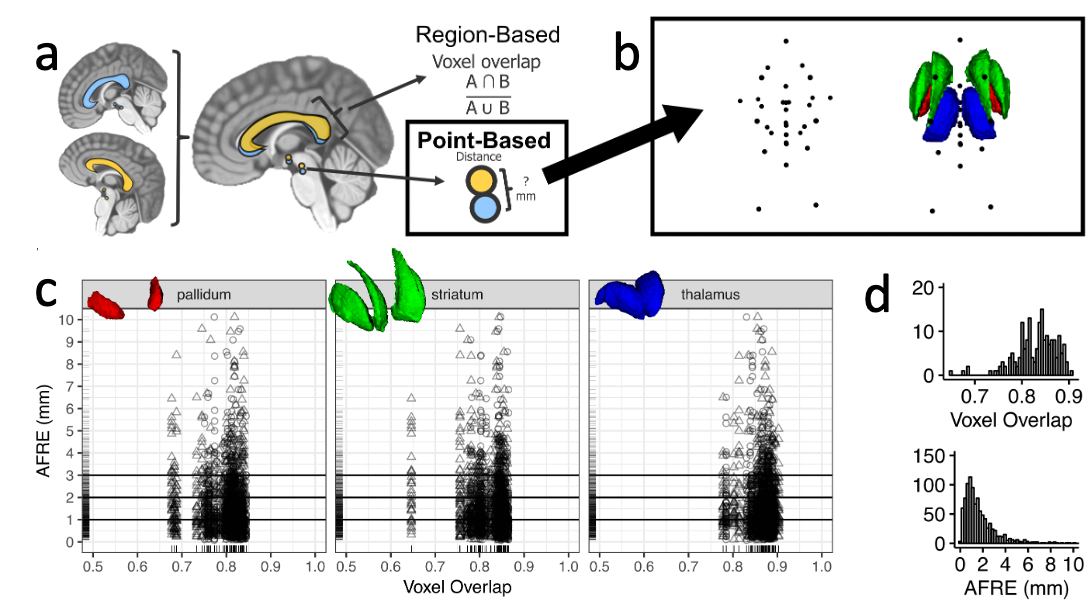
\includegraphics[width=1\linewidth]{figs/ch1_Figure_afidsvsoverlap.png}
    \caption{Head-to-head comparison of region-based overlap metrics and point-based metrics for evaluating spatial correspondence. (a) Schematic illustrating the computation of registration error metrics using either voxel-wise overlap between homologous regions (i.e., voxel overlap) and points (i.e., anatomical fiducial registration error; AFRE). (b) Abstraction of the anatomical fiducials (AFIDs) framework, with fiducial points distributed across three regions: pallidum (red), striatum (green), and thalamus (blue). (c,d) Trellis plots comparing region-based and point-based metrics. AFRE demonstrates a more unimodal distribution and a clearer, millimeter-scale dynamic range relative to voxel overlap metrics. Figure modified from an open-access article by \cite{Lau2019-eh}}
    \label{fig:ch1_Figure_afidsvsoverlap}
\end{figure}

\subsection{The Anatomical Fiducials Framework}
The Anatomical Fiducials (AFID) protocol is an open-access reference for the placement of fiducials in MRI \cite{Lau2019-eh}. These fiducials are defined based on reproducible neuroanatomical landmarks that span ventricular, sulcal, commissural, and deep brain regions. The goal of the protocol is to enable consistent and interpretable mapping of brain anatomy across individuals, imaging modalities, and spatial references (Figure .

Fiducials are placed manually by trained raters following a detailed anatomical definition guide, which includes visual references and 3D renderings to support accurate localization. Each AFID corresponds to a specific anatomical feature and is associated with a single point in the subject's native image space. The placement process typically requires a standard T1-weighted MRI scans, which provides sufficient contrast for identifying the underlying structure.

The resulting set of AFID coordinates forms a sparse point cloud that captures the spatial configuration of various areas of the brain. This point cloud can be used for a variety of downstream applications, including quality control of image registration, benchmarking of automated segmentation algorithms, and geometric morphometric analysis. Because AFIDs are interpretable and grounded in clearly defined anatomy, they are particularly well suited for assessing spatial transformations, including those involving deformation fields.

The AFIDs protocol has been validated in healthy controls and patient populations on T1w MRI, demonstrating inter-rater reliability on the order of 1-2 millimeters. Furthermore, it builds on open-source software infrastructures that support training, visualization, and analysis. The AFIDs protocol can become a valuable resource for researchers and clinicians seeking to quantify spatial accuracy and ensure anatomical fidelity in neuroimaging workflows.

\section{Machine Learning}
The field of neuroimaging has been transformed by the convergence of two powerful trends: (1) the availability of large-scale imaging datasets and (2) advances in computational methods. Open access datasets such as the Human Connectome Project (HCP; \cite{Van_Essen2013-yi}), UK Biobank \cite{Sudlow2015-lq}, Alzheimer's Disease Neuroimaging Initiative (ADNI; \cite{Petersen2010-rd}, and Parkinson's Progression Markers Initiative (PPMI; \cite{Marek2018-wx}) facilitated large-scale studies of brain structure, function, and disease. At the same time, improvements in computational resources—particularly the widespread availability of graphics processing units (GPU), high-performance computing clusters (HPC), and cloud-based infrastructure—have enabled the efficient training and deployment of complex machine learning (ML) models on high-dimensional neuroimaging data, dramatically accelerating both research and clinical translation \cite{Bouchard2016-cd,Kirimtat2024-is}.

\subsection{Overview of Machine Learning}
ML constitutes a methodologically diverse subfield of artificial intelligence that encompasses statistical techniques for developing computational algorithms capable of iterative self-improvement through data exposure and performance feedback \cite{Sarker2021-ng}. These algorithms demonstrate the capacity to recognize complex patterns, establish multidimensional relationships, and generate predictions from high-dimensional data without explicit rule-based programming \cite{Davatzikos2019-zq}.

ML operates through four fundamental processes: (1) Data preparation transforms raw input into suitable representations, often involving feature selection and normalization  \cite{Mwangi2014-nl}. (2) Model training adjusts parameters to minimize prediction errors on labeled examples, using optimization methods to find the best-fitting solution \cite{Lemm2011-jm}. (3) Regularization techniques balance the trade-off between fitting training data and maintaining generalizability to new examples \cite{Roberts2021-ib}. (4) Model inference tests performance on unseen data to ensure generalization beyond training examples, using metrics appropriate to the specific task \cite{Varoquaux2022-as}.  These processes work in concert to create systems that can recognize patterns and make predictions with increasing accuracy as they process more data.

ML methodologies are characterized by distinct learning paradigms based on the training data available and ultimate objective of the ML model. These paradigms are generally supervised, unsupervised, semi-supervised and reinforcement learning \cite{Hastie2009-ef}. \textbf{Supervised learning} optimizes algorithms using labeled training data, where each input is paired with corresponding output annotations; the algorithm learns to predict these outputs by minimizing the difference between its predictions and ground-truth labels. \textbf{Unsupervised learning} extracts intrinsic patterns from unlabeled data through dimensionality reduction or clustering algorithms, revealing underlying structures without predefined categories. \textbf{Semi-supervised learning} leverages both labeled and unlabeled data, addressing situations where annotations are limited while preserving generalization capabilities. \textbf{Reinforcement learning} enables algorithms to learn optimal behaviors through environmental interaction and feedback signals, its applications in medical imaging are limited compared to other paradigms \cite{Zhou2021-au}. 

These learning paradigms found natural applications in neuroimaging analysis, where the complexity and dimensionality of the data align with ML's pattern recognition strengths \cite{Vieira2017-vr}. The transition from general ML applications to medical imaging was particularly motivated by three factors:  (1) Standardized nature of medical image acquisition that facilitates algorithmic processing  \cite{Li2020-dy}. (2) Presence of anatomical patterns that remain relatively consistent across patients despite individual variations \cite{Iglesias2023-co}. (3) Potential for ML to address the time-intensive nature of manual image analysis in clinical workflows \cite{Khalifa2024-dn}. In the following sections, we outline the foundations of various ML models leveraged in this dissertation. 

\subsection{Traditional Machine Learning Models}
Traditional ML approaches in neuroimaging typically rely on handcrafted quantitative summary measures extracted from preprocessed scans using domain expertise and predefined anatomical or functional templates \cite{Mwangi2014-nl}. Common examples include regional brain volumes derived from segmentation protocols (e.g., hippocampal volume in Alzheimer’s disease), cortical thickness measurements from surface reconstructions (e.g., via FreeSurfer), white matter integrity metrics from DWI (e.g., fractional anisotropy), and voxel-wise signal intensities from structural or functional scans \cite{Abraham2014-va, Coupe2019-pe}. These features reduce the dimensionality of raw imaging data and make it more tractable for classical algorithms. Once extracted, these features are input into supervised learning algorithms (e.g., linear regression or random forests) which aim to map imaging-derived features to clinical or anatomical outcomes \cite{Mateos-Perez2018-xb,Jollans2019-mv,Sarica2017-dz}.

Ridge regression \cite{Hoerl1970-so} is a regularized linear model that addresses multicollinearity and overfitting by introducing an $\ell_2$ penalty on the magnitude of the regression coefficients. Given a dataset with input features $\mathbf{X} \in \mathbb{R}^{n \times p}$ and target vector $\mathbf{y} \in \mathbb{R}^n$, ridge regression estimates the coefficient vector $\boldsymbol{\beta} \in \mathbb{R}^p$ by minimizing the following objective function:

\begin{equation}
    \mathcal{L}_{\text{ridge}}(\boldsymbol{\beta}) = \|\mathbf{y} - \mathbf{X}\boldsymbol{\beta}\|_2^2 + \lambda \|\boldsymbol{\beta}\|_2^2,
\end{equation}

where $\lambda \geq 0$ is a regularization parameter controlling the trade-off between data fidelity and model complexity. This formulation encourages small coefficients and yields a stable solution even in the presence of many correlated predictors—a common scenario in neuroimaging applications where the number of features may exceed the number of samples.

In contrast, Extreme Gradient Boosting (XGBoost; \cite{Chen2016-ew}) is a nonlinear ensemble method based on gradient boosting of decision trees. It constructs a series of regression trees $\{f_m\}_{m=1}^M$, where each successive tree $f_m$ is trained to minimize the residual error of the current model:

\begin{equation}
    \hat{y}_i^{(m)} = \hat{y}_i^{(m-1)} + f_m(\mathbf{x}_i),
\end{equation}

and the overall objective includes a regularization term to penalize model complexity:

\begin{equation}
    \mathcal{L}_{\text{xgb}} = \sum_{i=1}^n \ell(y_i, \hat{y}_i) + \sum_{m=1}^M \Omega(f_m),
\end{equation}

where $\ell$ is a differentiable loss function (e.g., squared loss or logistic loss), and $\Omega(f_m)$ penalizes tree complexity (e.g., number of leaves and leaf weights). XGBoost can capture intricate nonlinear relationships and interactions between features, making it well-suited for high-dimensional imaging data with subtle and distributed signal patterns.

Both ridge regression and XGBoost are attractive in neuroimaging contexts due to their balance of performance, regularization control, and interpretability \cite{Rokem2020-vj,Yi2023-ak}. However, the performance of these models remains highly dependent on the quality and relevance of the chosen features \cite{Mwangi2014-nl}. Handcrafted features may fail to capture distributed or hierarchical patterns in the data, and models like ridge regression, while robust, assume linear relationships between inputs and outputs. Even flexible models like XGBoost, despite their ability to model nonlinearity, are only as powerful as the input features allow.

These limitations underscore the fact that traditional ML approaches, while foundational, are constrained by their indirect use of image data, their limited spatial expressiveness, and their dependence on predefined representations \cite{Varoquaux2022-as,Mwangi2014-nl}. This motivated the adoption of deep learning techniques \cite{Sarker2021-fo}, which seek to learn hierarchical and spatially grounded representations directly from raw neuroimaging data.

\subsection{Deep Learning Models}
\label{sec:deeplearning}
Deep learning (DL), a subfield of machine learning, enables models to learn hierarchical feature representations directly from raw data, removing the need for manual feature engineering \cite{LeCun2015-da, Sarker2021-fo}. Unlike traditional ML approaches that rely on predefined descriptors, DL models use multilayered artificial neural networks (ANNs) to automatically extract and combine increasingly abstract information through learned transformations. These networks are loosely inspired by the structure of biological neurons. The input is represented as a vector in the first layer of "neurons" and propagates through multiple hidden layers. Each neuron applies an affine transformation to the previous layer’s output followed by a nonlinear activation function:
\begin{equation}
    \mathbf{h}^{(l)} = \sigma\left( \mathbf{W}^{(l)} \mathbf{h}^{(l-1)} + \mathbf{b}^{(l)} \right),
\end{equation}

where $\mathbf{h}^{(l)}$ is the activation of layer $l$, $\mathbf{W}^{(l)}$ is the weight matrix, $\mathbf{b}^{(l)}$ is a bias vector, and $\sigma$ is a nonlinear function carefully chosen depending on application (e.g., Rectified Linear units or ReLU; \cite{Agarap2018-vg}). During training, these parameters are iteratively updated to minimize a task-specific loss function, allowing the model to build higher-level abstractions from raw input.

While effective for low-dimensional structured data, standard ANNs become impractical and do not account for the spatial structure of high-dimensional inputs such as 3D neuroimaging volumes. For example, flattening a \(64 \times 64 \times 64\) voxel patch would yield a 262,144-dimensional input vector, forcing each neuron in the first layer to learn a separate weight for every voxel. This results in massive parameter counts and a high risk of overfitting, while also discarding the spatial relationships inherent to image data. Convolutional neural networks (CNNs) address these issues using weight sharing and local receptive fields to preserve spatial structure while significantly reducing the number of learnable parameters \cite{LeCun2015-da,Indolia2018-vu}.

A CNN layer applies a learnable kernel \( w \in \mathbb{R}^{k \times k \times k} \) across the input volume via discrete convolution, producing feature maps that encode local spatial relationships. The output of a convolutional layer is given by:

\begin{equation}
    h^{(l)}_k = \sigma\left( \sum_{i=1}^{C^{(l-1)}} w^{(l)}_{ik} * h^{(l-1)}_i + b^{(l)}_k \right),
\end{equation}

where $h^{(l)}_k$ denotes the \(k\)-th feature map at layer \(l\), $*$ denotes convolution, and \(\sigma\) is an activation function. Deeper layers encode increasingly abstract representations by combining low-level features such as edges and textures into complex anatomical or pathological patterns.

One of the most influential architectures in biomedical image analysis is the U-Net \cite{Ronneberger2015-xm}, which uses an encoder–decoder structure to balance semantic context with spatial precision (Figure \ref{fig:ch1_Figure_UNET}). The encoder applies convolution and downsampling layers to extract global features, while the decoder path upsamples these features to recover spatial resolution using transposed convolutions. Crucially, skip connections between corresponding encoder and decoder layers allow early high-resolution features to be directly reused—preserving fine-grained spatial information that might otherwise be lost through pooling. Formally, the decoder reconstructs a segmentation map $\hat{Y} \in \mathbb{R}^{H \times W \times K}$ from a compressed latent representation $Z$ by applying learned upsampling operators:

\begin{equation}
    \hat{Y} = f_{\text{decoder}}(Z) = f^{(L)}_{\text{up}} \circ \cdots \circ f^{(1)}_{\text{up}}(Z),
\end{equation}

where each $f^{(i)}_{\text{up}}$ includes convolutional and skip-connection layers. The inclusion of skip connections between corresponding encoder and decoder levels allows the model to retain fine-grained spatial information that would otherwise be lost through pooling.

U-Nets are typically trained using voxel-wise loss functions such as cross-entropy or the Dice coefficient:

\begin{equation}
    \mathcal{L}_{\text{Dice}} = 1 - \frac{2 \sum_i p_i g_i}{\sum_i p_i + \sum_i g_i},
\end{equation}

where $p_i$ and $g_i$ represent predicted and ground truth labels for voxel $i$, respectively. Variants such as 3D U-Net \cite{Cicek2016-dz} and V-Net \cite{Milletari2016-ra} extend the architecture to volumetric data, and have become the standard for tasks such as skull stripping \cite{Hoopes2022-al} and segmentation \cite{Billot2023-tl, DeKraker2022-gj}. Contemporary improvements include the incorporation of residual blocks, attention modules, and multi-scale feature fusion to improve robustness in low-contrast or morphologically variable regions \cite{Oktay2018-rh}. 

\begin{figure}[hbt!]
     \centering
     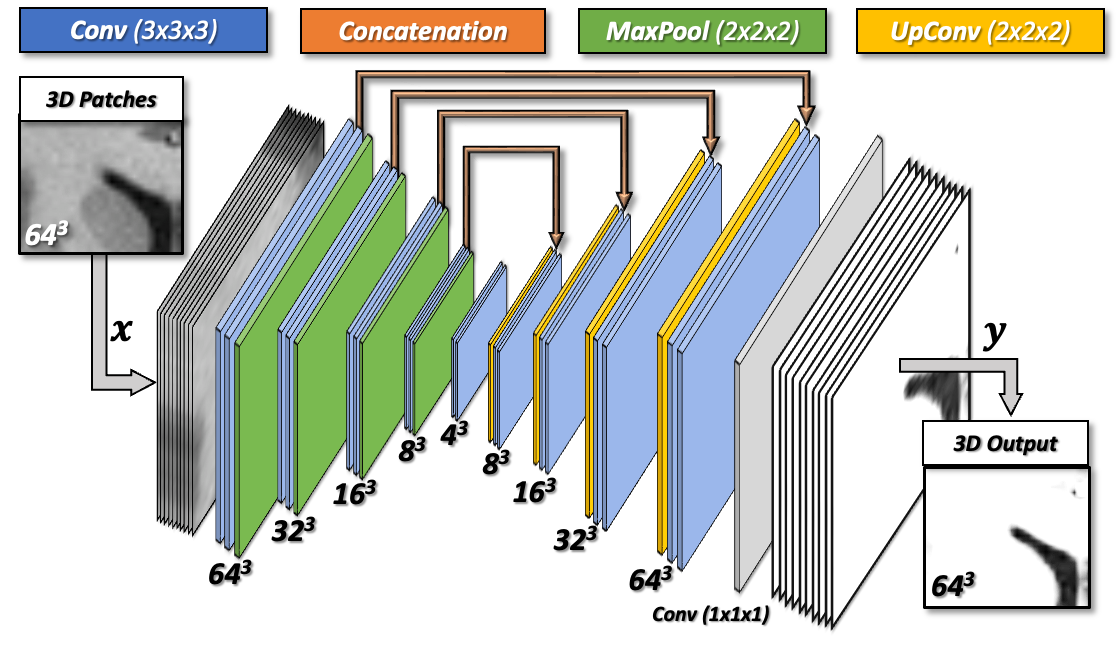
\includegraphics[width=1\linewidth]{figs/ch1_Figure_UNET.png}
     \caption{Schematic of an example 3D U-Net architecture \cite{Ronneberger2015-xm,Cicek2016-dz} used for volumetric image-to-image prediction. The input consists of $64^3$ voxel 3D patches, which undergo repeated convolution operations (blue; $3{\times}3{\times}3$ kernels) and spatial downsampling via max pooling (green; $2{\times}2{\times}2$). The encoder-decoder structure enables feature extraction at multiple scales, with skip connections (orange) preserving spatial information through concatenation. The decoder path applies upconvolutions (yellow; $2{\times}2{\times}2$) to restore resolution and generate the final $64^3$ voxel 3D output which depicts a brain ventricle segmentation as way of example.}
     \label{fig:ch1_Figure_UNET}
 \end{figure} 
 
Further advancements include nnU-Net \cite{Isensee2021-ev}, a self-configuring deep learning framework for biomedical image segmentation. Unlike traditional approaches that require manual tuning of preprocessing, network architecture, and training parameters, nnU-Net automates these decisions based on dataset-specific properties. Upon receiving a new dataset, nnU-Net analyzes its characteristics—such as image modality, size, and spacing—and configures a tailored segmentation pipeline. This includes selecting appropriate network architectures (e.g., 2D, 3D, or cascaded U-Nets), preprocessing steps, and post-processing techniques. This holistic approach has enabled nnU-Net to achieve state-of-the-art performance across 23 public datasets, surpassing many specialized methods with minimal manual intervention.

Although architectures such as U-Net were originally developed for image segmentation, they have also been adapted for point-based tasks such as anatomical landmark detection \cite{Ertl2025-wu,Chong2024-rp,Ye2023-wn}. Compared to segmentation, landmark detection in neuroimaging presents unique challenges: (1) Anatomical landmarks in brain MRI are often small and situated in regions of low contrast or homogeneous intensity. Many correspond to subtle anatomical features or geometric constructs, such as the midpoint of a structure or the intersection of internal axes, rather than distinct visual boundaries. Consequently, models must infer these points from contextual cues rather than relying on strong local image features. (2) Landmark detection involves predicting a highly localized signal against a vast background, leading to extreme class imbalance. Without careful loss function design or architectural modifications, models may converge to trivial solutions. These characteristics have motivated specialized network designs and training strategies that output spatial coordinates—either directly through coordinate regression heads \cite{Nibali2018-bu} or indirectly via heatmap prediction \cite{Payer2016-ik}.

\subsection{Challenges in Generalization and Interpretability}
Despite their promise, traditional ML and DL models face significant challenges in clinical neuroimaging. A major concern is generalization: models trained on data from a specific scanner, protocol, or population may not perform well when deployed in a different setting \cite{Davatzikos2019-zq}. Neuroimaging datasets are heterogeneous, where subtle differences in acquisition parameters can introduce bias. Efforts such as domain adaptation, harmonization, and transfer learning attempt to mitigate these effects, but the problem remains a barrier to clinical deployment \cite{Iglesias2023-co}. Furthermore, Many DL models function as "black boxes" that provide predictions without a clear explanation of their basis without explicit design \cite{Holzinger2019-kw}. This opacity can undermine clinician trust and complicate error analysis. Techniques such as saliency mapping, attention mechanisms, and feature attribution have been proposed to improve interpretability, but these methods may lack the spatial or clinical grounding necessary for anatomically meaningful insights \cite{Dinsdale2022-hf}.

\section{Open Science and Brain Imaging Data Structure}

Reproducibility and transparency are foundational to modern neuroimaging research, particularly as studies increasingly span large, heterogeneous datasets and complex analytical pipelines. The work in this dissertation embraces open science principles through the use of open data structures and code, version-controlled data management, and workflow automation tools that support reproducibility at scale.

\subsection{Brain Imaging Data Structure}

The Brain Imaging Data Structure (BIDS) \cite{Gorgolewski2016-oh} provides a standardized format for organizing and describing neuroimaging datasets. By specifying consistent directory hierarchies, file naming conventions, and metadata formats across imaging modalities, BIDS facilitates automated analysis, data sharing, and interoperability across tools. All imaging data used in this dissertation—including structural MRI volumes and anatomical fiducial annotations—are organized in BIDS-compliant formats and released openly. To manage datasets in a reproducible and decentralized manner, we adopt \texttt{datalad} \cite{Halchenko2021-px}, a data version control system that extends Git and Git-annex for large scientific datasets. \texttt{Datalad} enables efficient tracking of changes to imaging data, annotations, and model outputs across multiple machines and collaborators.

\subsection{Workflow Management}
As neuroimaging datasets grow in complexity and scale, reproducible and modular workflow management has become essential to ensure transparency and efficiency in data processing. Workflow engines provide a structured approach to defining and executing analytical pipelines, making it easier to track dependencies, scale computations, and share methods. In this work, we make use of \texttt{Snakemake} \cite{Molder2021-ig,Koster2012-ok}, a widely used workflow management system, together with \texttt{Snakebids} \cite{Van-Dyken-Tristan-Kuehn-Jason-Kai-Dahananjhay-Bansal-Ali-Khan2020-ay}, a companion interface that simplifies working with BIDS-organized neuroimaging data.

This BIDS-compliant framework provides a robust and extensible foundation for open, scalable, and reproducible neuroimaging research. By adhering to established standards and publicly releasing all data, code, and models, this dissertation contributes to the broader neuroimaging ecosystem—extending its utility to applications in stereotactic neurosurgery.

\section{Thesis Outline and Objectives}

This dissertation addresses the challenge of localizing brain structures with millimetric accuracy in a way that is scalable, interpretable, and clinically actionable. Deep brain stimulation surgery underscores the need to solve this challenge, where therapeutic targets such as the subthalamic nucleus are small, functionally heterogeneous, and situated within densely packed subcortical regions. Precise targeting is essential, yet the surgical planning process often relies—either directly or indirectly—on population-based maps generated through nonlinear image registration. These frameworks can introduce spatial errors on the same order as the targets themselves, complicating both individual treatment and broader scientific inference. At the same time, these same registration-based approaches are foundational to population neuroscience, where imaging data from many individuals is warped into a common stereotactic space to study brain structure, variability, and disease. In both settings—clinical and research—spatial uncertainty undermines confidence in localization and limits the translation of group-level findings to individual patients.

\begin{figure}[hbt!]
    \centering
    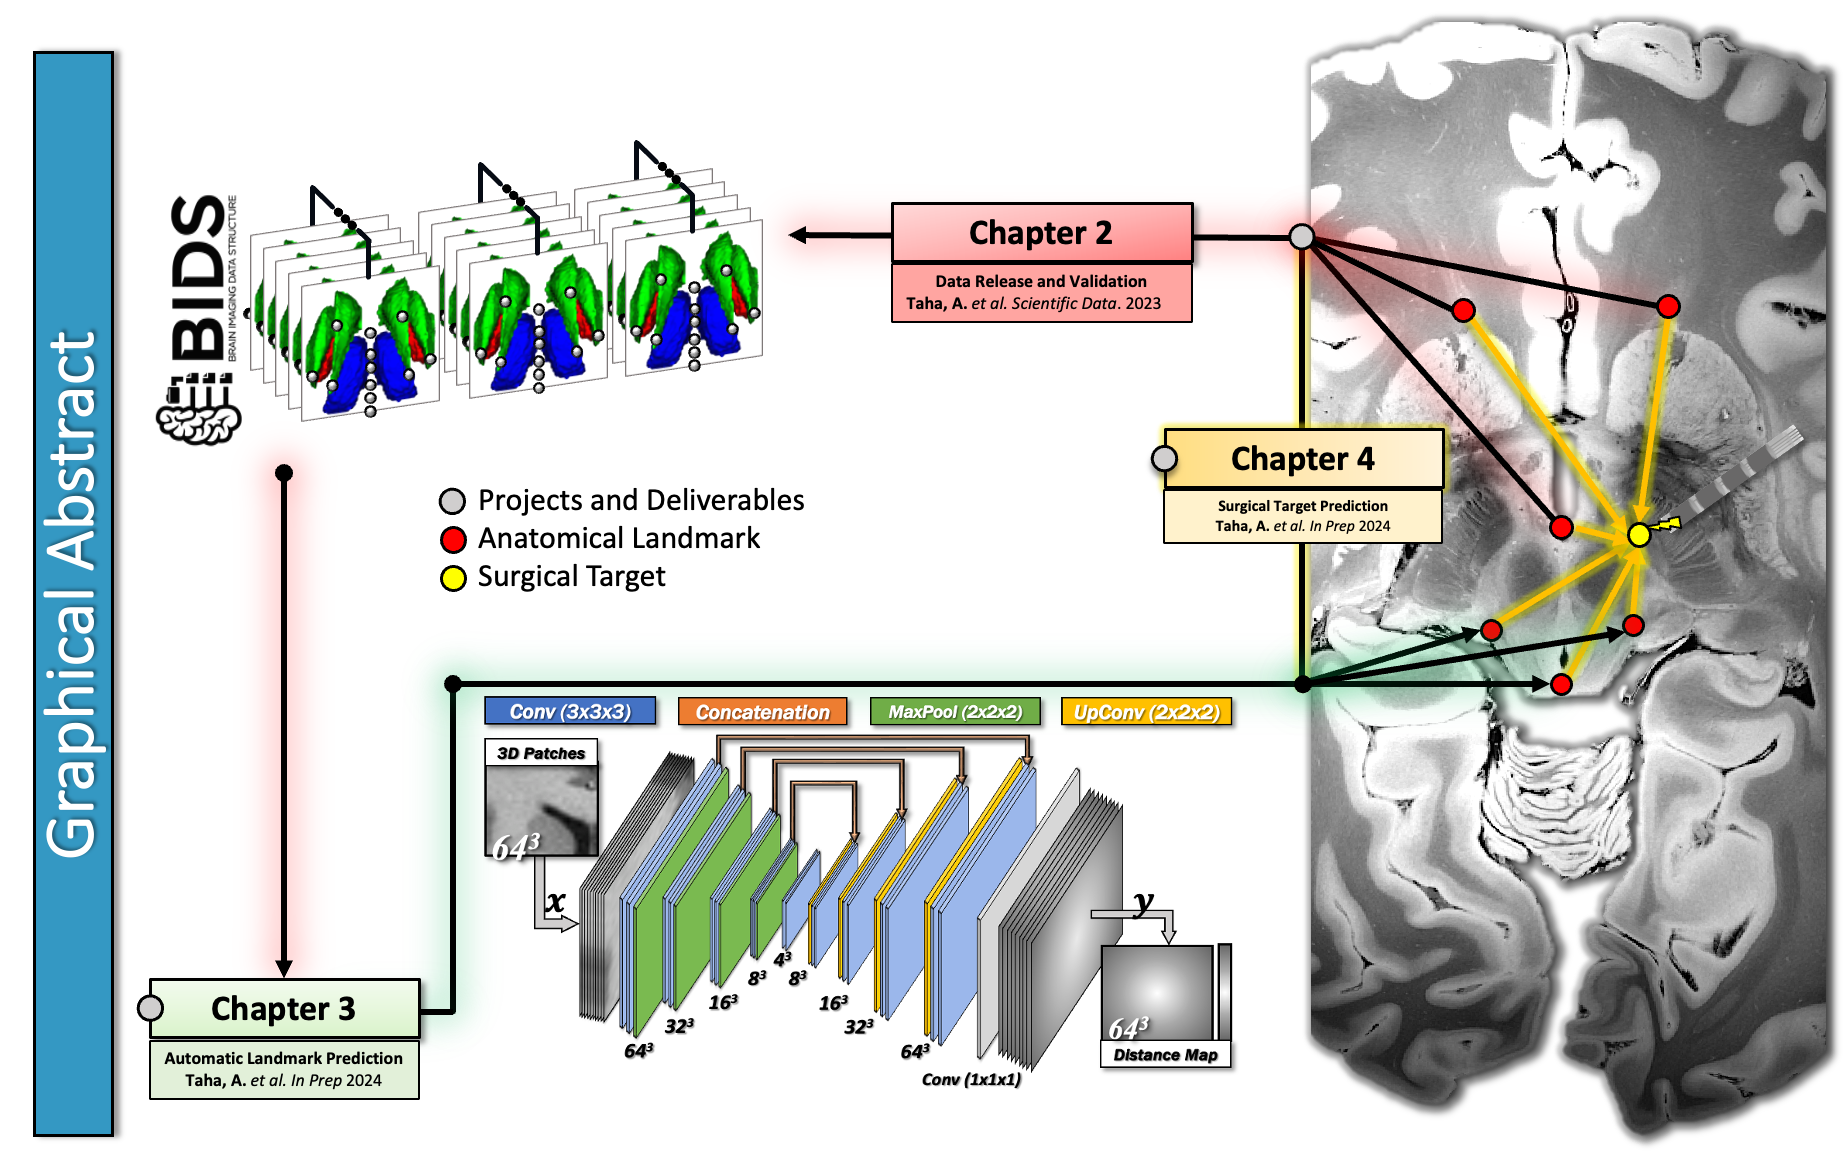
\includegraphics[width=1\linewidth]{figs/ch1_Figure_Abstract.png}
    \caption{Graphical abstract of dissertation projects. \textit{Chapter 2} is focused on validation of a brain landmark annotation protocol and open release of data. \textit{Chapter 3} employs deep learning to automatically localize brain landmarks in an open-source implementation. \textit{Chapter 4} is focused on leveraging data and models from prior chapters to solve the deep brain stimulation target localization problem.}
    \label{fig:Abstract}
\end{figure}


This dissertation introduces a coordinate-based framework inspired by classical stereotactic principles and enhanced by modern machine learning to support spatially precise and interpretable workflows in neuroimaging and neurosurgery (Figure \ref{fig:Abstract}). We demonstrate how brain coordinates can be used to improve quality control and brain mapping in \textit{Chapter 2}, automate anatomical landmark detection in \textit{Chapter 3}, and predict the location of deep brain targets on clinical MRI in \textit{Chapter 4}. Together, these tools support surgical targeting and reliable population-level analyses. The specific objectives of each chapter are as follows:
\begin{itemize}
\item \textbf{\textit{Chapter 2}}: Validation of the Anatomical Fiducials (AFIDs) protocol—a standardized set of 32 anatomical landmarks—on multi-resolution structural MRI and the open release of annotated AFID datasets to support reproducibility and benchmarking.
\item \textbf{\textit{Chapter 3}}: Development of a modular, open-source pipeline for automatic AFID placement using machine learning with accuracy competitive to that of human raters.
\item \textbf{\textit{Chapter 4}}: Leverage AFID-derived geometry to predict the location of surgical targets and validate model generalizability across MRI modalities and field strengths.
\end{itemize}
\chapter{AFIDs-Data: MRI datasets with anatomical fiducial annotations}\label{chap:afidsdata}
\newpage
\sloppy

\noindent This chapter is largely based on:
\begin{itemize}[noitemsep,topsep=0pt]
	\item Taha, G. Gilmore, M. Abbass, et al. Magnetic resonance imaging datasets with anatom-
ical fiducials for quality control and registration. Scientific Data, 10:449, 2023.
\end{itemize}

\section{Background and Summary}
Tools available for reproducible, quantitative assessment of brain correspondence have been limited. The anatomical fiducial (AFID) placement protocol was developed and validated for millimetric accuracy in image registration. This chapter presents curated AFID placements for widely-used structural MRI datasets and templates. The data includes 132 subjects across four datasets (15,232 fiducials) and 14 templates (4,288 fiducials), totaling over 300 hours of annotation. Human rater accuracy is validated to be within 1--2 mm using over 45,000 Euclidean distances. The datasets conform to the Brain Imaging Data Structure (BIDS) format.

\section{Current Applications}
\subsection{Registration Assessment}
Curated AFIDs are released for diverse datasets and templates, enabling testing and validation of registration algorithms. Example use cases include deformable template creation and error quantification using AFIDs, supporting both linear and non-linear methods.

\subsection{Education}
The AFID framework enables neuroanatomy teaching. New raters can compare their placements to the normative data using the AFIDs validator. The tool offers visual documentation, upload capabilities, and real-time feedback.

\subsection{Brain Structure and Volumetric Analyses}
AFID placements support morphological comparisons, aiding biomarker identification in neurodegenerative diseases.

\section{Prospective Applications}
\subsection{Registration Optimization and Quality Control}
Curated datasets allow head-to-head comparison of registration methods and can be integrated into development workflows.

\subsection{Automatic and Accurate Landmark Placement}
AFIDs serve as ground truth for machine learning models that aim to automate fiducial localization.

\subsection{Surgical Targeting}
Ultra-high field MRI (e.g., 7T) provides visibility into small structures such as the STN. AFIDs aid predictive modeling for target localization.

\subsection{Brain Anatomy Abstraction and Anonymization}
AFID-based coordinate systems allow anonymized yet anatomically relevant analyses, facilitating pooling of datasets.

\section{Methods}
\subsection{Fiducial Selection and Placement Assessments}
The AFID protocol comprises 32 landmarks across midline and bilateral locations. Fiducials are chosen to be robust across 1.5T, 3T, and 7T MRIs.

\subsection{Hardware and Software}
Placements were done using 3DSlicer, primarily the Markups Module. Points are placed in native space and saved as \texttt{.fcsv} files.

\subsection{Performing the AFID Protocol}
Raters underwent training via live tutorials and online resources. The placements began with AC and PC points, followed by midline and lateral structures. Annotations deviating from $>$ 10 mm were excluded.

\subsection{Dataset Descriptions}
\textbf{AFIDs-HCP30}: 30 unrelated healthy subjects (3T scans), annotated by five expert raters.

\textbf{AFIDs-OASIS30}: 30 subjects from OASIS-1 (age 25--91), annotated by one expert and two novices per scan.

\textbf{LHSCPD}: 40 Parkinson's patients (1.5T), annotated by two experts and three novices.

\textbf{SNSX}: 32 healthy controls imaged at 7T. Annotated by one expert and two novices per scan.

\subsection{Template Descriptions}
\textbf{MNI2009bAsym, Agile12v2016, MNIColin27}: Annotated by the same raters as AFIDs-OASIS30.

\textbf{BigBrainSym, MNI2009bSym, PD-25}: Annotated by two expert raters.

\textbf{TemplateFlow (8 templates)}: Annotated by one expert and three novices.

\subsection{AFLE Calculation}
Mean AFLE is computed as the average Euclidean distance from each rater placement to the ground truth per fiducial. Inter-rater AFLE is the average pairwise distance between raters.

\section{Data Records}
All placements (19,520 total AFIDs) and imaging data are shared in BIDS format. Data is hosted across Zenodo and OpenNeuro repositories. Raw and ground truth placements are provided as \texttt{.fcsv} files.

\section{Technical Validation}
Global mean AFLE was  mm. Placement accuracy was reproducible across datasets and raters. See for metrics.

\section{Usage Notes}
We recommend using 3DSlicer to load the shared \texttt{.fcsv} annotation files and their corresponding MRI images. Instructions for dataset access are included in the central repository: \url{https://github.com/afids/afids-data}.

Text here and a reference. Also another reference cited in Chapter \ref{chap:intro}.

\subsection{Some equation}

Text here with an equation.

\begin{equation}
\begin{aligned}
\underset{p_S,p_T,q,\lambda} \min & \int_\Omega p_S(x)dx \\
\text{s.t. } & |q'(x)| \leq R(x) , \\
\text{ } & \lambda(x) \geq 0, \\
\text{ } & p_S(x) \leq D_S(x), \, p_T(x) \leq D_T(x), \\
\text{ } & \operatorname{div}\left( q'(x) + \lambda(x)e(x) \right) - p_S(x) + p_T(x) = 0
\label{eq:jingOpt}
\end{aligned}
\end{equation}
where $D_S(x)$ and $D_T(x)$.


\chapter{AutoAFIDs: Automatic Anatomical Fiducial Localization} \label{chap:AutoAFIDs}
\newpage
\sloppy
This chapter is largely based on:
\begin{itemize}[noitemsep,topsep=0pt]
	\item Taha, A., Bansal, D., Snyder, M., et al. AutoAFIDs: Automatic brain landmark detection for quality control, stereotactic targeting, and brain charting. In Preparation.
\end{itemize}

\section{Introduction}
\subsection{Brain Coordinates in Neuroimaging and Neurosurgery}
Three-dimensional Cartesian coordinates (x, y, z) offer a convenient and precise framework to represent brain structures. This abstraction underlies a broad range of applications in both neuroimaging and neurosurgical workflows, enabling reproducibility \cite{Dockes2020-nw}, cross-subject comparison \cite{Glasser2016-ko}, and multimodal data integration \cite{Uludag2014-qz}. In research, coordinates form the backbone of meta-analytic platforms such as \texttt{NeuroSynth} \cite{Yarkoni2011-sr} and \texttt{NeuroQuery} \cite{Dockes2020-nw}, which aggregate reported coordinates from thousands of studies to identify consistent associations between brain and behavior. In clinical contexts, neuromodulation targets and optimal stimulation zones are represented by coordinates relative to the major anatomical landmarks \cite{Horn2017-bi} such as anterior and posterior commissure (AC and PC), guiding trajectory planning and enabling retrospective outcome analysis. Across both domains, coordinates are a shared spatial language for modeling and navigating the brain.

\subsection{Automatic Landmark Localization}
The manual localization of brain landmarks is often time-intensive, cognitively demanding, and subject to inter-rater variability \cite{Abbass2022-lf, Lau2019-eh,Pallavaram2008-zr}. Even with detailed annotation protocols, raters require training to achieve consistency \cite{Lau2019-eh}. These challenges pose a barrier to scaling coordinate-based workflows across large datasets and neuroimaging pipelines. To address this bottleneck, deep learning (DL) methods offer a promising avenue for automatic landmark detection in brain MRI. These approaches typically fall into two paradigms: (1) coordinate regression \cite{Neupane2024-vt} and (2) heatmap-based localization \cite{Payer2016-ik}. In coordinate regression, a network directly outputs the x,y,z coordinates of each landmark (often via fully connected layers or global pooling). In heatmap-based methods, the network predicts a probability map (often a Gaussian “fuzzy” blob) for each landmark, and the peak of the heatmap is taken as the location. Heatmap regression has become especially popular because it retains spatial context and allows the network to localize landmarks in a fully convolutional manner.

\subsection{Deep Learning Approaches}
DL has significantly advanced the field of computer vision by enabling end-to-end learning of hierarchical features directly from data, leading to substantial improvements in tasks such as facial landmark detection, pose estimation, and image registration \cite{Lathuiliere2018-oy}. While medical imaging adopted these tools more gradually, fully convolutional networks—particularly U-Net and its 3D variants—have since become foundational for segmentation and anatomical localization tasks \cite{Akkus2017-eh, Falk2019-us}. Variants such as V-Net and cascaded U-Nets improve spatial precision by capturing both global context and local detail, while architectures like the spatial configuration network (SCN) \cite{Payer2016-ik, Payer2019-sn} and multi-task cascaded CNNs \cite{Zhang2017-dc} embed geometric priors to enhance performance in data-scarce settings. More recently, self-configuring pipelines like nnLandmark \cite{Ertl2025-wu} and attention-based models such as H3DE-Net \cite{Huang2025-vt} have streamlined deployment and improved model efficiency. Despite these advances, relatively limited studies have adapted such innovations to the detection of brain landmarks central to stereotactic targeting and coordinate-based neuroimaging \cite{Edwards2021-su}. Given their consistent anatomy and clinical importance, AC-PC detection represents a promising use case for applying modern deep learning techniques to improve automation, reproducibility, and standardization in brain mapping workflows.

\subsection{Limitations in the field}
Several barriers limit the broader utility of these DL techniques. First, well-annotated, publicly available datasets with standardized brain landmarks remain scarce, which constrains training, benchmarking, and validation. Second, many existing models are not open-source, are difficult to reproduce, or lack adherence to FAIR (Findable, Accessible, Interoperable, and Reusable; \cite{Wilkinson2016-it}) data principles. Third, to the best of our knowledge, no automated workflows are built in environments compatible with the Brain Imaging Data Structure (BIDS; (Gorgolewski et al., 2016)), which impedes integration with modern neuroimaging pipelines and limits accessibility for the broader scientific community. As a result, the full potential of automated coordinate-based analysis for applications such as registration quality control, brain morphometry, or lifespan brain charting remains underrealized.

\subsection{Our Proposed Approach}
In this work, we present \texttt{AutoAFIDs}, a BIDS-App for automatic landmark detection using deep learning. We trained and tested \texttt{AutoAFIDs} using a curated open-access dataset of MRI scans (n = 202) across a range of MRI field strengths (1.5, 3, and 7T) and conditions (healthy, abnormal ventricles, and neurodegenerative) with 20,000+ landmarks manually localized by human raters. \texttt{AutoAFIDs} demonstrated a landmark localization accuracy comparable to human raters. We also demonstrate the broad utility of \texttt{AutoAFIDs} for two downstream applications which we make available to end-users: 1) quality control of image registration, 2) stereotactic target localization. By applying \texttt{AutoAFIDs} on over 2,000 MRI scans from individuals aged 18 to 100, we uncovered millimetric differences in brain structure that distinguish healthy brain changes from early signs of neurodegenerative disease.

\section{Methods}
\subsection{Problem Definition}
\label{sec:problemstatement}
The objective of this study was to localize anatomical fiducial points distributed across multiple brain regions using a supervised deep learning framework. Let $\mathcal{V} \subset \mathbb{R}^3$ denote a 3D brain volume, and let $\{p_1, p_2, \ldots, p_L\}$ represent the set of $L$ target landmark coordinates, where each $p_\ell \in \mathbb{R}^3$ denotes the location of the $\ell^{\text{th}}$ anatomical point of interest.

We formulated this as a regression problem in which the model learns to predict a smooth, continuous-valued distance map centered on the target landmark. For each voxel $v \in \mathcal{V}$ and landmark $\ell$, the ground truth target $D^\ell(v)$ is defined as:

\begin{equation}
D^\ell(v) = \lVert v - p_\ell \rVert_2
\end{equation}

To enhance stability and spatial resolution, we applied an exponential decay to the predicted distance map:

\begin{equation}
T^\ell(v) = \exp(-\alpha \cdot D^\ell(v))
\end{equation}

where $\alpha$ is a fixed scaling factor controlling the spatial decay rate. During training, the model learns to predict this transformed image using a mean squared error (MSE) loss between the predicted image \( \hat{T}(v) \) and the ground-truth target \( T(v) \) across all voxels \( v \) in the prediction region \( \mathcal{V} \):

\begin{equation}
\mathcal{L} = \frac{1}{|\mathcal{V}|} \sum_{v \in \mathcal{V}} \left( \hat{T}(v) - T(v) \right)^2
\end{equation}

Here, \( \mathcal{V} \) denotes the set of voxels within the input patch or volume, \( T(v) \) is the ground-truth voxelwise signal derived from the known landmark coordinate, and \( \hat{T}(v) \) is the model’s prediction at voxel \( v \). This formulation enables dense supervision and encourages the model to produce spatially coherent predictions with millimetric localization accuracy.


\subsection{Imaging and Coordinate Data}

We made use of landmarks defined by the Anatomical Fiducials (AFIDs) protocol, a standardized set of 32 brain landmarks manually placed on structural T1-weighted MRI scans \cite{Lau2019-eh}. These fiducials span diverse anatomical regions, including subcortical nuclei, ventricular boundaries, and midline structures such as the anterior and posterior commissures. The imaging acquisition protocols, annotation procedures, and coordinate data used here are described in detail in Chapter~\ref{chap:afidsdata} but shown in Figure \ref{fig:ch3_Figure_data} for completeness.

For model development, all curated datasets were divided into training ($n = \textbf{148}$), validation ($n = \textbf{42}$), and testing ($n = \textbf{21}$) subsets. Stratified splitting of each dataset was used to ensure representative anatomical and demographic diversity across all sets.

\begin{figure}[hbt!]
    \centering
    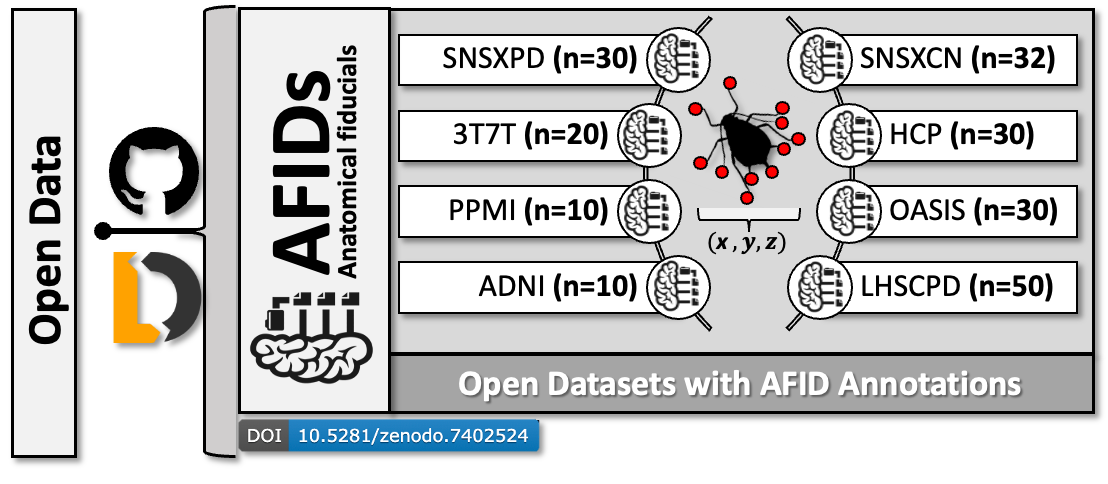
\includegraphics[width=1\linewidth]{figs/ch3_Figure_data.png}
    \caption{We made use of a previously released dataset containing anatomical fiducial (AFID) annotations. This dataset comprises eight sub-datasets spanning a range of MRI field strengths and neurodegenerative conditions. For machine learning modeling, we apply a stratified 70/20/10 split into training, validation, and test sets. By training on the combined heterogeneous dataset, the model is encouraged to learn features that are agnostic to imaging resolution, field strength, and MRI acquisition parameter differences.}
    \label{fig:ch3_Figure_data}
\end{figure}

\subsection{Preprocessing and Data Preparation}

We adopted standardized preprocessing profiles inspired by the nnU-Net framework \cite{Isensee2021-ev}, with additional modifications tailored for anatomical landmark detection. We built our workflow within a BIDS-compliant Snakemake \cite{Koster2012-ok} pipeline integrating with PyBIDS \cite{Yarkoni2019-lu} (i.e., SnakeBIDS; \url{https://github.com/khanlab/snakebids}). Input data were T1-weighted (T1w) structural MRIs, optionally converted from alternate contrasts (e.g., T2w, FLAIR, CT) using SynthSR \cite{Iglesias2023-co} when specified. 

\begin{figure}[hbt!]
    \centering
    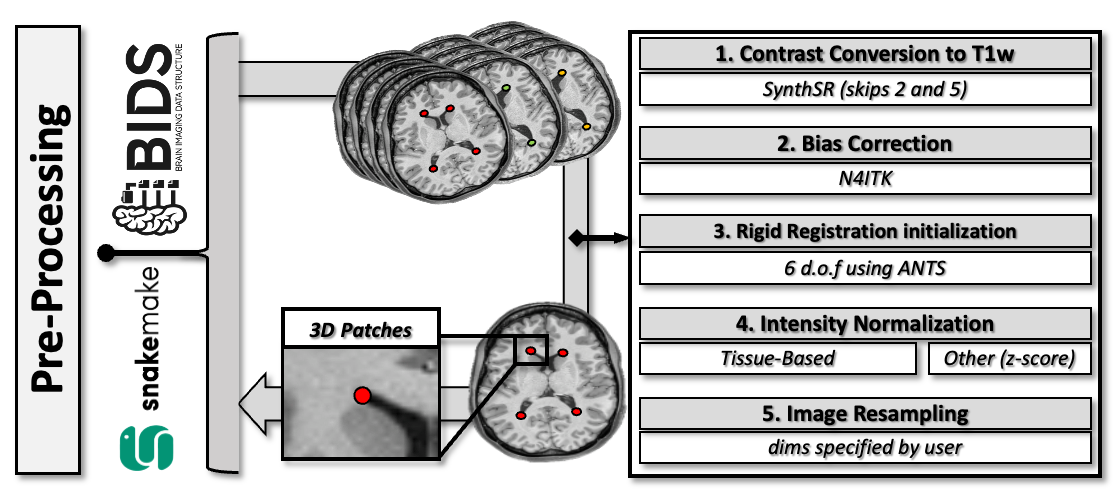
\includegraphics[width=1\linewidth]{figs/ch3_Figure_proc.png}
    \caption{Overall preprocessing pipeline employed in \texttt{AutoAFIDs}. Preprocessing is generally modality specific but centered around processing T1w MRI. We make use of (1) SynthSR \cite{Iglesias2023-co} to convert various modalities (e.g., T2w, CT, or FLAIR) to T1w image. Subsequently, a T1w image goes through the following preprocessing steps: (2) bias correction \cite{Tustison2010-qu}, (3) rigid registration of an annotated template for landmak priors, (4) MRI volume intensity normalization performed using various user-specified options and finally (5) resampling of the MRI volume to an isotropic resolution. The SynthSR model already outputs images that do not need to undergo preprocessing steps 2 and 5.}
    \label{fig:ch3_Figure_proc}
\end{figure}


All T1w MRI scans undergo the following steps:

\begin{enumerate}
    \item \textbf{Bias field correction:} N4 bias field correction \cite{Tustison2010-nw} is applied to mitigate intensity non-uniformities arising from scanner-related artifacts.
    
    \item \textbf{Intensity normalization:} Image intensities are normalized on a per-volume basis using robust z-score normalization, enhancing contrast between tissue boundaries relevant for landmark detection. However, we also provide the option of min-max normalization.
    
    \item \textbf{Isotropic resampling:} All volumes are resampled to a uniform 1~mm isotropic resolution to ensure consistent spatial scaling across subjects.
    
    \item \textbf{Template-to-subject registration:} A rigid registration of the MNI152NLin2009cAsym template to each subject’s native space is performed using ANTs \cite{Avants2011-zs}. This transformation is applied only to restrict the inference search space and guide patch sampling, without altering anatomical label coordinates.
    
    \item \textbf{Patch extraction:} Volumes are divided into 3D patches centered around the expected landmark region. This local patching strategy reduces memory demands and encourages finer localization.
    
    \item \textbf{Spatial augmentation:} During training, 3D patches are augmented via random rigid rotations. Each rotation is applied about a uniformly sampled axis with an angle drawn from a normal distribution with zero mean and standard deviation $\sigma_{\text{angle}}$ (in degrees), promoting rotational robustness.
\end{enumerate}

Ground-truth heatmaps for each landmark are generated by computing the voxel-wise Euclidean distance (ED) to the target coordinate and applying an exponential decay function as described in Section \ref{sec:problemstatement}.

\subsection{Patch-Based Inference}

Rather than processing the entire volume, the model predicts landmarks using a patch-based strategy. For each target landmark $\ell$, we extract a cubic patch of size $2r+1$ centered on a prior coordinate $p_\ell^{\text{prior}}$ obtained by registering a standard template (e.g., MNI space) to the subject’s native image. Let $\mathcal{P}_\ell$ denote the local patch centered on $p_\ell^{\text{prior}}$:

\begin{equation}
\mathcal{P}_\ell = \left\{ v \in \mathcal{V} \ \middle|\ \lVert v - p_\ell^{\text{prior}} \rVert_\infty \leq r \right\}
\end{equation}

The input to the network is a single-channel image patch, and the output is a distance map over $\mathcal{P}_\ell$. The predicted landmark $\hat{p}_\ell$ is extracted as the centroid of the thresholded exponential-transformed output:

\begin{equation}
\hat{p}_\ell = \text{centroid} \left( \left\{ v \in \mathcal{P}_\ell \ \middle|\ \exp(-\alpha \cdot \hat{D}^\ell(v)) > \tau \right\} \right)
\end{equation}

where $\tau$ is a percentile-based threshold (e.g., top 1\%) applied to suppress noisy responses and extract a coherent region.

\subsection{Model Architecture and Training}

Each landmark is predicted using a separate deep neural network trained independently. The shared architecture is a lightweight 3D U-Net implemented in TensorFlow. Training was performed using the Adam optimizer with early stopping on a validation set. The loss function is mean squared error between the predicted and target distance maps (after exponential transform), as described above.

\begin{figure}[hbt!]
    \centering
    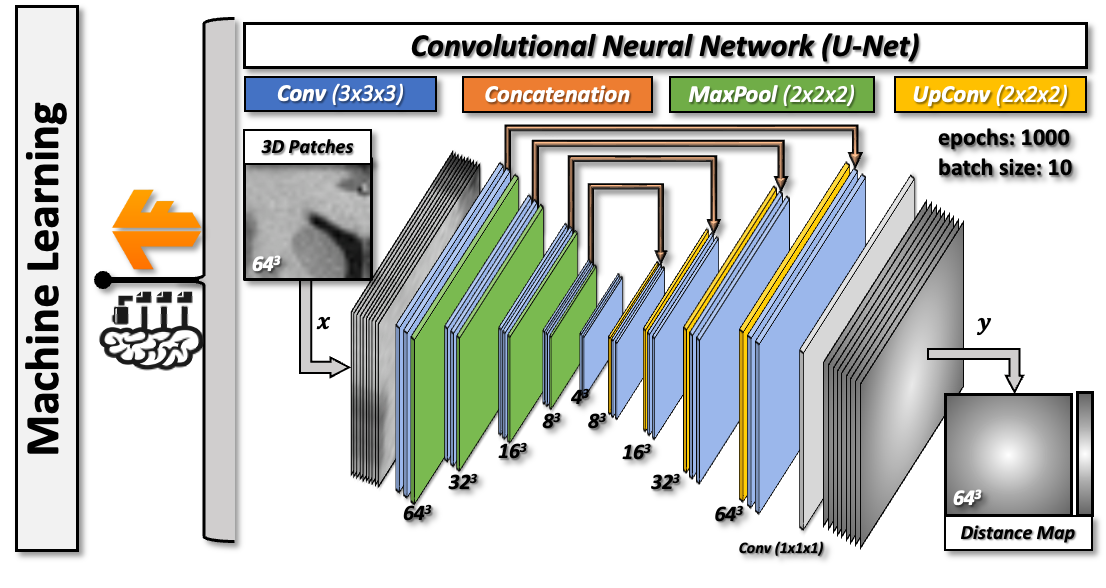
\includegraphics[width=1\linewidth]{figs/ch3_Figure_cnn.png}
    \caption{Overview of the deep learning model architecture used for anatomical fiducial localization. The model is a 3D U-Net that takes as input a 3D patch centered around a prior landmark location. The network consists of convolutional blocks (Conv, 3×3×3), downsampling via max-pooling (2×2×2), and upsampling via transposed convolutions (UpConv, 2×2×2). Skip connections concatenate encoder and decoder feature maps to preserve spatial detail. The output is a single-channel distance map representing the ED from each voxel to the target anatomical landmark.}
    \label{fig:ch3_Figure_cnn}
\end{figure}


\subsection{Model Design Rationale}
In this work, we adopt a one-network-per-landmark training strategy. While many existing approaches predict all landmarks jointly using a multi-channel output architecture, we opt for training separate models for each anatomical point. This decision is motivated by two key considerations.

First, the anatomical heterogeneity of the landmarks poses a significant modeling challenge. The AFIDs span multiple tissue types and spatial contexts—including landmarks adjacent to ventricles, embedded within white matter tracts, and lying on cortical gray matter surfaces. These diverse appearance profiles often demand different spatial priors and texture sensitivities, which a shared model may struggle to learn simultaneously. Training distinct models allows each network to specialize in the local anatomical context of its assigned landmark, without interference from competing objectives. Second, certain use cases—such as deep brain stimulation (DBS)—require sub-voxel precision in landmark localization. Errors of just a few millimeters can lead to clinically significant deviations in surgical targeting or trajectory planning. In such high-stakes applications, even minor improvements in accuracy for individual landmarks can have meaningful downstream impact. By isolating each landmark into its own dedicated model, we maximize the opportunity for hyperparameter tuning, data augmentation, and architectural adaptation tailored to each target's anatomical and clinical importance. Together, these considerations justify a modular, per-landmark approach that prioritizes accuracy and adaptability over computational efficiency.

\section{Results}
\subsection{Landmark Localization Accuracy}
Model performance was evaluated on a held-out test set (n = 21) by computing the ED between predicted and ground truth AFID coordinates (see Table \ref{fig:ch3_Figure_autoscore}). Across all 32 anatomical landmarks (672 predictions in total), the model achieved high spatial accuracy, with a median ED of 1.21 mm and an interquartile range (IQR) of 0.76–1.95 mm. Per-landmark performance showed modest variability, reflecting differences in anatomical complexity, tissue contrast, and inter-subject variability. Ten landmarks exhibited median errors in the sub-millimetric range (0.4–0.9 mm), while more challenging regions, such as those adjacent to ventricular structures, demonstrated higher variability (2-2.4 mm). The maximum observed error across all landmarks was 5.28 mm. A complete summary of per-landmark accuracy is provided in Table~\ref{tab:autoafids_accuracy}.

\begin{figure}[hbt!]
    \centering
    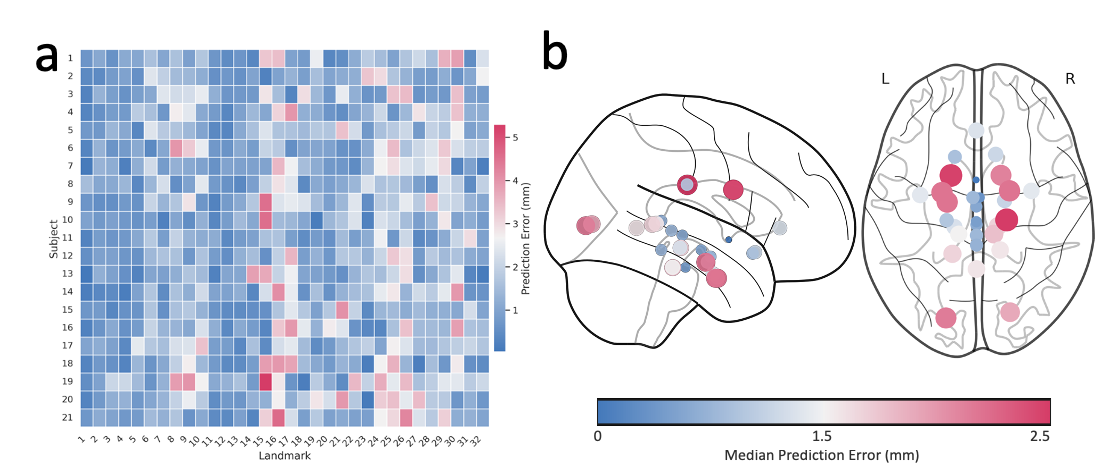
\includegraphics[width=1\linewidth]{figs/ch3_Figure_autoscore.png}
    \caption{Overview of localization error using \texttt{AutoAFIDs}. (a) Heatmap showing Euclidean distance errors (in mm) for each predicted anatomical landmark across 21 test subjects. Each column corresponds to one of the 32 AFIDs, and each row to a subject. (b) Spatial distribution of landmark-specific median prediction errors visualized on a glass brain. Each point represents the anatomical location of an AFID in stereotactic space, with marker size and color encoding the median error across subjects. Highter spatial variability in model accuracy was observed in lateral and ventricular landmarks.}
    \label{fig:ch3_Figure_autoscore}
\end{figure}

\subsection{Registration Evaluation Using \texttt{AutoAFIDs}}
To assess the utility of \texttt{AutoAFIDs} for evaluating registration quality, we compared its predicted landmark coordinates to those derived from \texttt{Lead-DBS} (v3.0; \cite{Neudorfer2023-wd}), a widely used software suite for DBS research that incorporates multi-stage nonlinear registration to align patient MRI data to MNI space. 

\begin{figure}[hbt!]
    \centering
    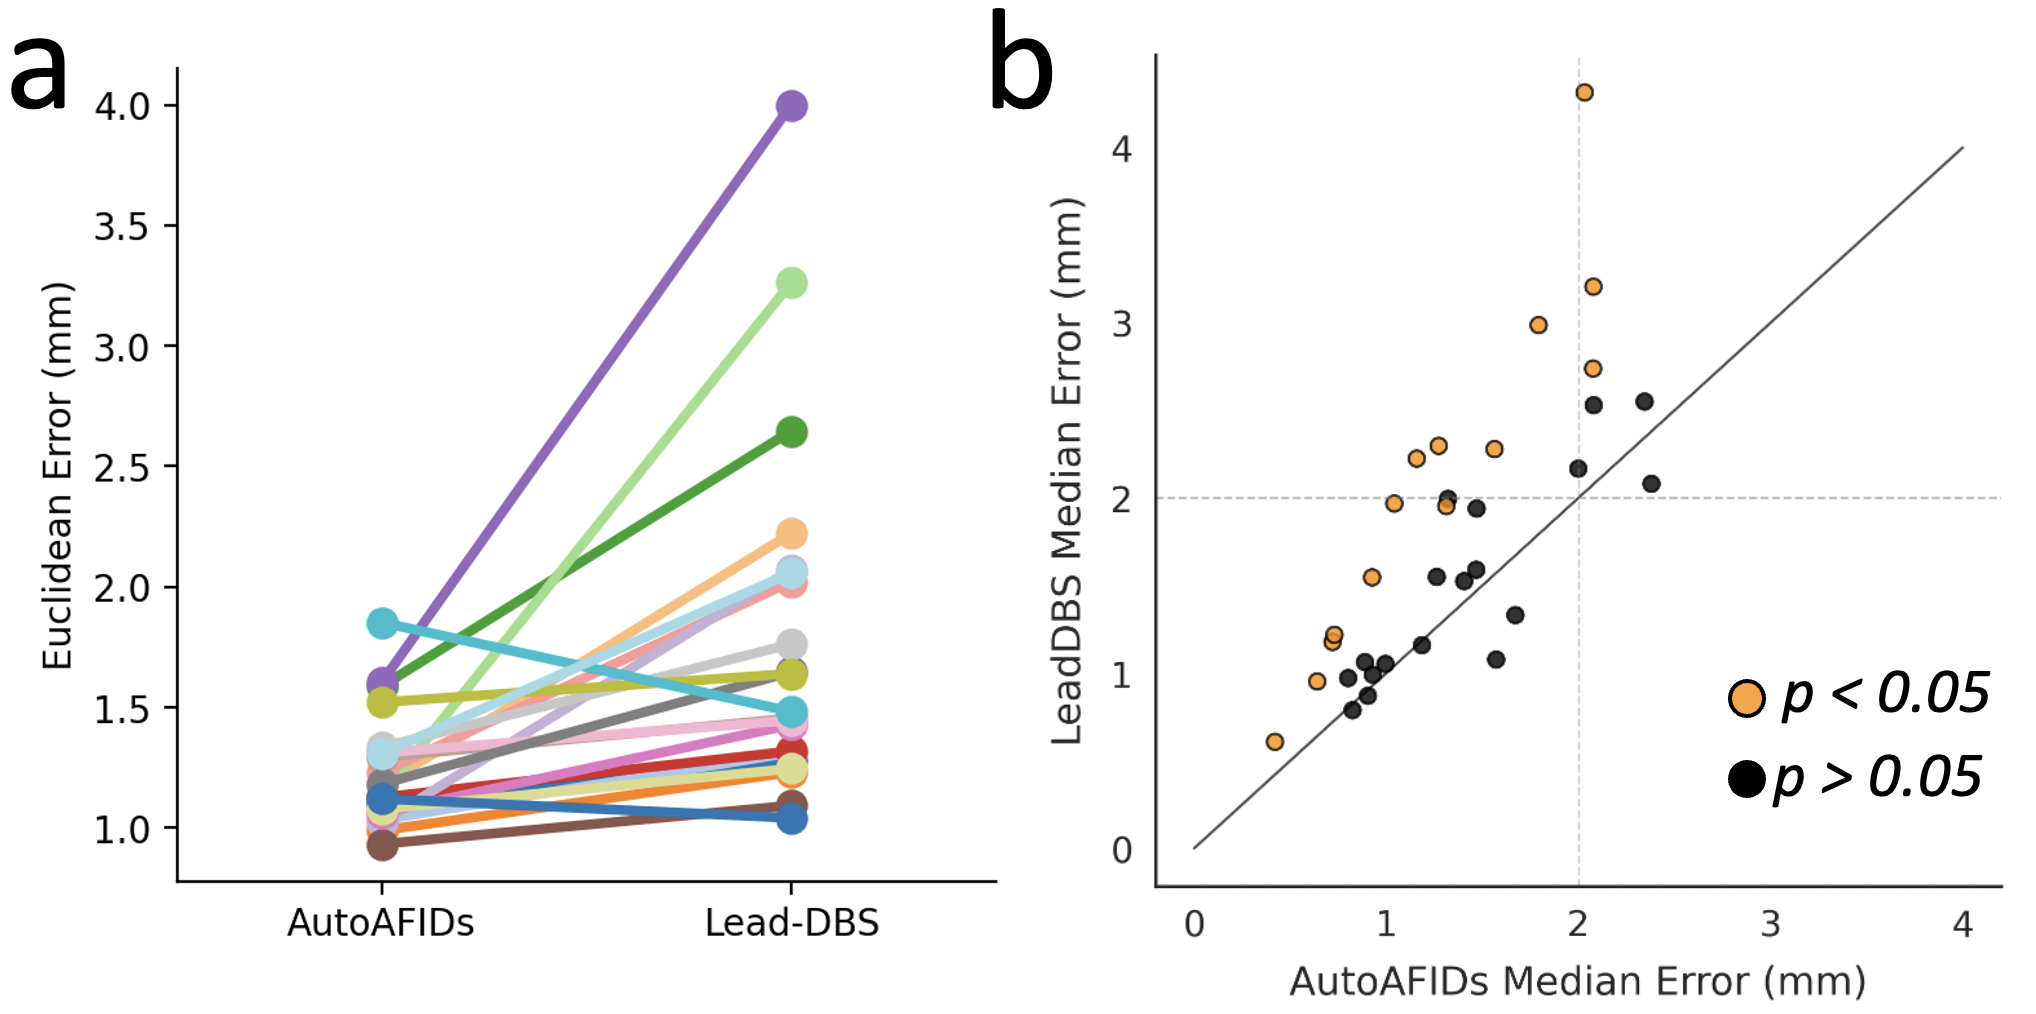
\includegraphics[width=0.95\linewidth]{figs/ch3_Figure_cnnvslead2.png}
    \caption{Comparison between \texttt{AutoAFIDs} and \texttt{Lead-DBS} at landmark localization in native space. (a) Subject-wise median Euclidean distance (ED) errors across all landmarks. (b) Landmark-wise comparison of median ED for \texttt{AutoAFIDs} versus \texttt{Lead-DBS}. Points are colored by Wilcoxon signed-rank test significance. (c) Distribution of all EDs for \texttt{AutoAFIDs} (red) and \texttt{Lead-DBS} (blue), shown as overlapping histograms and cumulative frequency curves. Vertical dashed lines indicate medians.}
    \label{fig:ch3_Figure_cnnvslead}
\end{figure}

For both methods, subject-level median ED errors were computed across all 32 AFIDs, resulting in 21 paired measurements per method. The median ED across subjects was 1.21 mm for \texttt{AutoAFIDs} and 1.71 mm for \texttt{Lead-DBS}. A Wilcoxon signed-rank test revealed a statistically significant difference in localization error (p\(<\)0.001), indicating superior performance by \texttt{AutoAFIDs}. The distribution of subject-level and AFID-level errors is visualized in Figure~\ref{fig:ch3_Figure_cnnvslead}a and b, respectively. \texttt{AutoAFIDs} statistically outperformed \texttt{Lead-DBS} in 14 out of 32 AFIDs. Figure~\ref{fig:ch3_Figure_cnnvslead}c shows the full distribution of all landmark EDs and their cumulative frequencies.

Motivated by the variability observed in registration performance, we developed an automated QC application that uses \texttt{AutoAFIDs} to generate subject-specific summaries of registration accuracy. For each subject, our registration quality control tool computes descriptive statistics of ED across all 32 AFIDs. A qualitative review panel presents slice-wise visualizations for each AFID at cardinal planes with crosshairs centered on the registered and reference landmark coordinates. The report also includes a heatmap summarizing localization error by coordinate axis (x, y, z) and a 3D scatterplot visualizing landmark displacement between stereotactic space and the registered subject image. These features enable users to identify individual landmarks with high registration error, assess global alignment patterns, and quickly spot outliers. A sample report is provided in Figure~\ref{fig:figuresupregqc}.

\subsection{Brain Charting Using \texttt{AutoAFIDs}}

To explore how structural brain variability is encoded in pairwise AFID distances (Figure \ref{fig:ch3_Figure_pairwisedata}a), we analyzed a lifespan dataset of 2,834 subjects from nine publicly available neuroimaging cohorts (Figure \ref{fig:ch3_Figure_pairwisedata}b). Subjects ranged in age from 18 to 100 years, with an approximately even sex distribution (50.6\% female; Figure \ref{fig:ch3_Figure_pairwisedata}c) and broad diagnostic coverage (Figure \ref{fig:ch3_Figure_pairwisedata}d), including 2,000 cognitively normal (CN) individuals (70.6\%), 650 with Parkinson’s disease (PD, 22.9\%), and 184 with Alzheimer’s disease (AD, 6.5\%). AutoAFID annotations were successfully generated for all subjects, resulting in 496 pairwise distances per scan derived from 32 AFIDs. We apply a sex-stratified interquartile range (IQR; thresholded at 5 standard deviations) method to identify and remove outlier values for each distance feature, excluding extreme anatomical deviations likely to arise from poor AFID localization.

We first applied t-distributed stochastic neighbor embedding (t-SNE) to the standardized pairwise distance matrix to visualize population-level structure (Figure~\ref{fig:ch3_Figure_tsne}a-d). When colored by sex and age, the t-SNE embedding revealed a smooth gradient, suggesting that these demographic factors represent principal axes of anatomical variation within the AFID feature space. We observed modest separation by disease status, indicating potential disease-related morphometric signatures. In contrast, no clear clustering was observed by imaging site, suggesting that AFID-based morphometry is relatively robust to differences in image acquisition protocols.

\begin{figure}[hbt!]
    \centering
    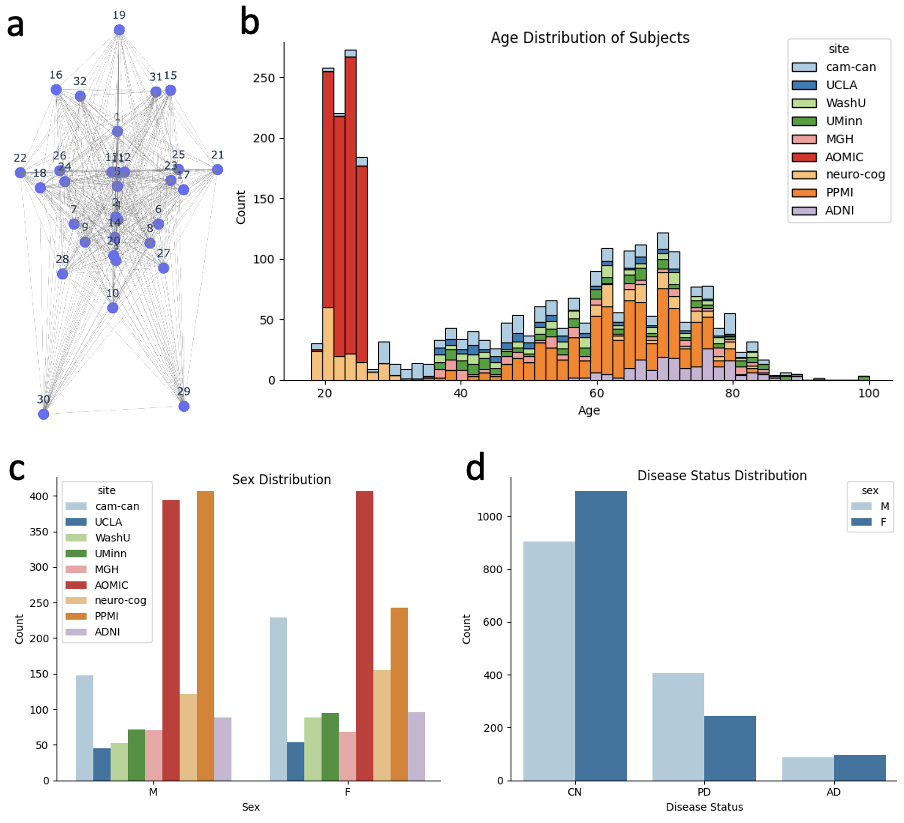
\includegraphics[width=1\linewidth]{figs/ch3_Figure_pairwisedata.png}
    \caption{(a) 3D plot showing all 496 pairwise connections between the 32 anatomical fiducials (AFIDs), illustrating the dense spatial sampling achieved across the brain. (b) Age distribution of subjects stratified by imaging site, demonstrating broad lifespan coverage and diverse dataset contributions. (c) Sex distribution by site, indicating approximate sex balance across most cohorts. (d) Distribution of subjects by disease status and sex, showing that the majority of participants are cognitively normal (CN), with additional representation from Parkinson’s disease (PD) and Alzheimer’s disease (AD) groups.
}
    \label{fig:ch3_Figure_pairwisedata}
\end{figure}

To examine how specific brain distances change across the lifespan, we computed Pearson correlations between each pairwise AFID distance and age among cognitively normal (CN) individuals. The top 10 positively and negatively correlated features are shown in Figure~\ref{fig:ch3_Figure_tsne}f,g. Several inter- and intra-regional distances demonstrated strong age dependence. The most positively correlated features primarily involved midline and posterior structures (e.g., AFID 13 to 12, 13 to 11), suggesting age-related expansion or elongation in these regions. Conversely, negatively correlated features predominantly involved anterior and subcortical structures (e.g., AFID 5 to 3, 3 to 2), indicating localized contraction or atrophy with age. These patterns reflect nonuniform aging trajectories across brain regions and highlight the sensitivity of coordinate-based morphometry to capture biologically meaningful structural changes.

\begin{figure}[hbt!]
    \centering
    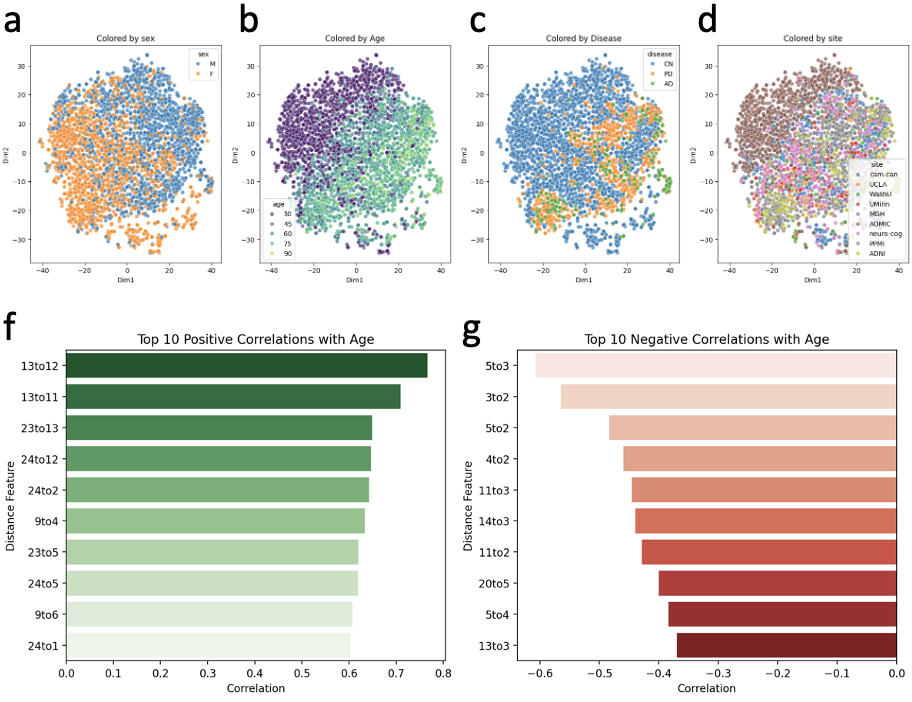
\includegraphics[width=1\linewidth]{figs/ch3_Figure_tsne.png}
    \caption{t-distributed stochastic neighbor embedding (t-SNE) embedding and age-related correlations in AFID distance space. (a–d) Two-dimensional t-SNE projection of subjects based on standardized AFID pairwise distances. Each point represents a subject and is colored by (a) sex, (b) age, (c) disease status, or (d) acquisition site. A clear gradient is observed along the age axis (b), while sex, disease, and site show limited separability, suggesting that age is the dominant source of variation in the AFID feature space. (f–g) Bar plots showing the top ten AFID pairwise distances with the strongest Pearson correlations with age. (f) Positively correlated distances primarily involve the mammillary bodies and temporal horn fiducials, reflecting expansion of periventricular and CSF spaces with age. (g) Negatively correlated distances involve brainstem and midbrain fiducials, potentially reflecting age-related compaction or atrophy along the brainstem axis.
    }
    \label{fig:ch3_Figure_tsne}
\end{figure}

We specifically examined age-related changes in the anterior commissure–posterior commissure (AC–PC) distance, given their central role as key landmarks in stereotactic neurosurgery. Across cognitively normal individuals, we observed a small but consistent increase in AC–PC length with age in both sexes (Figure~\ref{fig:ch3_Figure_acpc}). Males had longer AC–PC distances than females (median ± IQR: 26.63 ± 1.48 mm vs. 25.81 ± 3.04 mm, respectively). In the PD subgroup, AC–PC distances were generally longer than in cognitively normal individuals. Males also had a longer AC-PC distance than females, median of 28.22 ± 5.14 mm vs. 27.25 ± 3.76 mm, respectively. To account for potential confounding by age, we performed age-matched comparisons of AC–PC distance between CN individuals and those with PD using a Mann-Whitney U test. Even after matching, AC–PC distances remained significantly longer in the PD group (p \(<\) 0.001), suggesting disease-associated structural changes along this canonical axis. This reinforces the relevance of individualized targeting in stereotactic applications where the AC–PC line serves as a key anatomical reference.

\begin{figure}[hbt!]
    \centering
    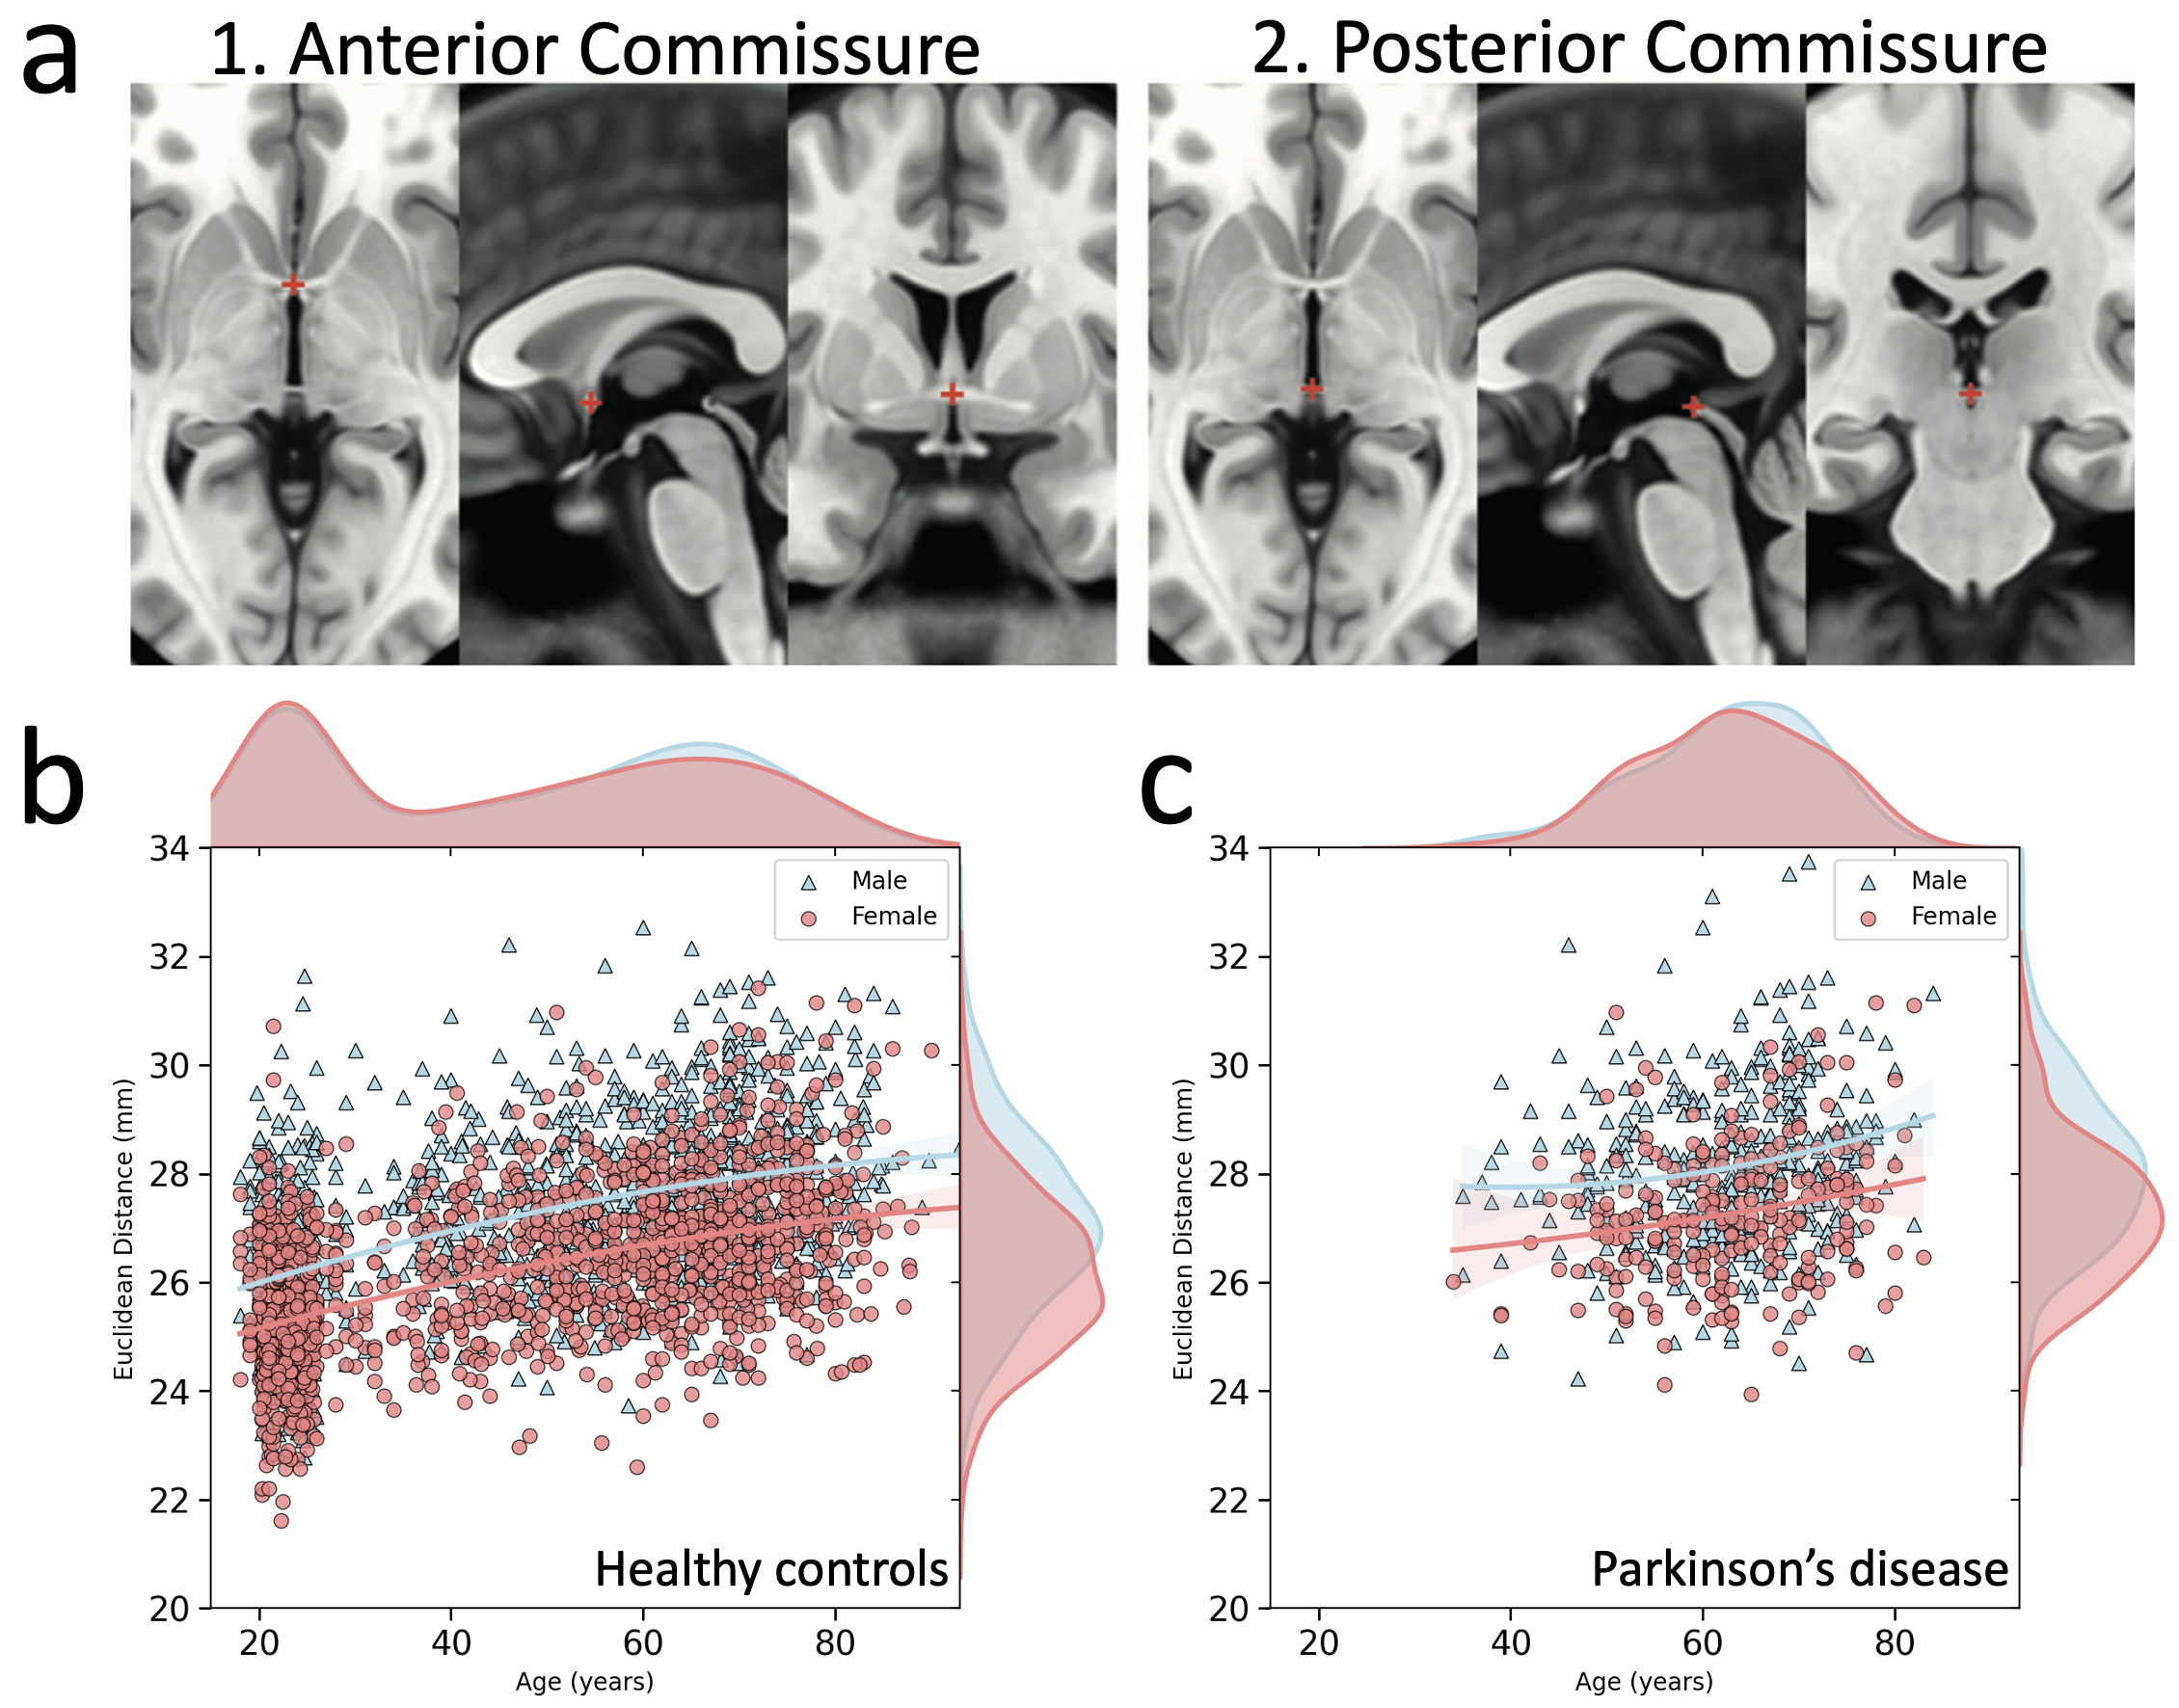
\includegraphics[width=1\linewidth]{figs/ch3_Figure_acpc.png}
    \caption{
    Analysis of the anterior commissure–posterior commissure (AC–PC) line across age and disease. (a) Anatomical definition of the AC (left) and PC (right) landmarks shown in axial, sagittal, and coronal views. (b) Age-related trends in AC–PC distance among cognitively normal cohort. A subtle increase in distance is observed with age, with males showing longer distances than females. (c) AC–PC distances in individuals with Parkinson’s disease. A similar age-related trend is observed. Shaded bands represent 95\% confidence intervals for sex-stratified second-order polynomial fits.
    }
    \label{fig:ch3_Figure_acpc}
\end{figure}

\section{Discussion}
In this study, we introduce \texttt{AutoAFIDs}, an open-source deep learning-based framework for automatic localization of anatomical fiducials (AFIDs) with millimetric accuracy. Our data and code is designed for generalizability, enabling incorporation into various software compatible with the BIDS specification. \texttt{AutoAFIDs} can quality control registration and capture morphometric changes in the human brain. This work introduces a novel framework for stereotactic brain charting across the human lifespan, which we leverage to characterize morphometric changes in neurodegenerative disease.

\subsection{Landmark Localization Performance}

\texttt{AutoAFIDs} achieved a median Euclidean distance (ED) of 1.21 mm (IQR: 0.76–1.95 mm) across 32 AFIDs in a held-out test set of 21 subjects. These results are in line with the range reported for similar tasks \cite{Ertl2025-wu, Salari2024-iu, Edwards2021-su} and approach expert-level precision (0-2 mm), particularly for brainstem landmarks \cite{Abbass2022-lf}. Ten of the 32 AFIDs showed sub-millimetric median errors, while more anatomically variable regions, such as those near the ventricles, exhibited higher variability. This was also consistent with prior reports of inter-rater localization accuracy \cite{Lau2019-eh, Abbass2022-lf}. Although we did not perform a direct comparison between \texttt{AutoAFIDs} and inter-rater localization accuracy, we direct the reader to Chapter \ref{chap:afidsdata} where we provide a breakdown of inter-rater localization accuracy across all AFID datasets. 

Several competing models for landmark localization in brain MRI offer direct points of comparison, as they make use of the AFIDs data released in Chapter~\ref{chap:afidsdata}. Among them, \texttt{nnLandmark} \cite{Ertl2025-wu} reported an average localization error of approximately 1.27 mm. However, accuracy per landmark was not reported, limiting insight into how the model performs across anatomically diverse regions, particularly in challenging areas near the ventricular system. Given that \texttt{nnLandmark} also employs a U-Net architecture, the overall similarity in accuracy is expected. A notable limitation of the model is the lack of a released codebase and the absence of compatibility with the BIDS specification. This increases the technical burden for neuroimaging researchers and developers, who must independently integrate model inference into large-scale, BIDS-compliant workflows. \texttt{DeepNavNet} \cite{Edwards2021-su}, which uses a 3D residual network architecture, focuses on localizing the anterior and posterior commissures for neuronavigation. \cite{Edwards2021-su} reported localization errors of 0.79 ± 0.33 mm and 0.78 ± 0.33 mm for the AC and PC respectively. These results are comparable to the performance of \texttt{AutoAFIDs} for the same landmarks (AC: 0.42 mm, PC: 0.83 mm), demonstrating competitive accuracy even relative to models specialized for only two targets. In contrast, \cite{Salari2024-iu} developed \texttt{CABLD}, a contrast-agnostic self-supervised approach to landmark regression that involves annotating a single reference example. While this flexibility is notable, the reported accuracy of \texttt{CABLD} is on the order of 3–4 mm. This level of performance is insufficient for millimetric applications such as registration quality control, where we show that even established nonlinear pipelines like \texttt{Lead-DBS} achieve median landmark alignment errors around 1.7 mm. The lower accuracy of \texttt{CABLD}, therefore, restricts its utility in precision-demanding use cases.

A key strength of \texttt{AutoAFIDs} lies in the design of the system, where each landmark is treated as a separate supervised learning task with its own dedicated model. This modular, per-landmark approach allows new anatomical targets to be easily added to the framework without retraining the entire system. It also enables more tailored optimization for each landmark, which may be especially important for landmarks with distinct spatial or contrast features. Another advantage of \texttt{AutoAFIDs} is its modular and user-facing configuration (see Supplementary content~\ref{app:yaml}), which is compatible with the BIDS specification. To our knowledge, no current BIDS-aware tools exist in the literature for brain landmark localization. This flexibility, combined with consistent sub-millimetric to low-millimetric accuracy, positions \texttt{AutoAFIDs} as a scalable tool for brain mapping and surgical planning.

\subsection{Evaluation of Registration Accuracy}

We benchmarked \texttt{AutoAFIDs} against \texttt{Lead-DBS}, a widely adopted pipeline for nonlinear registration in DBS research. \texttt{AutoAFIDs} significantly outperformed \texttt{Lead-DBS} on landmark localization accuracy across subjects and AFIDs (p\(<\)0.001), with superior performance in 14 of 32 landmarks. This suggests that direct landmark prediction may complement or even surpass deformation-based alignment in capturing subject-specific anatomical variability. It is also important to note that \texttt{Lead-DBS} employs a rigorously validated registration scheme and was curated by comparisons of six modern and established algorithms \cite{Ewert2019-cc}. Thus, \texttt{Lead-DBS} serves as a strong benchmark for comparison, though it may overestimate the performance of general-purpose in-house registration tools. Beyond group-level accuracy, \texttt{AutoAFIDs} also provides a valuable framework for registration quality control by generating intuitive, subject-specific visualizations and quantitative error summaries. To our knowledge, no existing open-source tools offer automatic and reproducible quantitative metrics for evaluating registration accuracy; most neuroimaging software still relies on qualitative visual inspection. By enabling the detection and quantification of misalignments, \texttt{AutoAFIDs} promotes greater transparency and accountability in image preprocessing—an increasingly important consideration as neuroimaging and neurosurgical workflows become more reliant on automated pipelines.

\subsection{Structural Brain Charting Across the Lifespan}
We demonstrated that pairwise distances between AFIDs, automatically predicted using \texttt{AutoAFIDs}, capture meaningful structural variation across the human lifespan and provide a robust framework for population-level morphometric analysis. By analyzing 2,834 MRIs from nine diverse public neuroimaging cohorts, we show that coordinate-based representations of brain anatomy can encode individual differences related to age, sex, and disease status, while remaining resilient to variability in imaging site and acquisition protocol.

Dimensionality reduction via t-SNE revealed that age and sex are principal axes of variation in the AFID-derived feature space, consistent with prior studies that report global and regional brain volume changes associated with these demographic factors \cite{Fjell2010-aq, Ritchie2018-df}. The continuous age gradient observed in the embedding indicates that AFID pairwise distances encode smooth anatomical changes across the lifespan, likely reflecting progressive atrophy, ventricular expansion, and sulcal widening. Notably, the minimal clustering by acquisition site supports the modality-agnostic potential of this framework, underscoring its utility for multi-cohort studies where scanner variability often confounds traditional voxelwise analyses \cite{Fortin2018-ke}.

Our correlation analysis of cognitively normal individuals identified both positive and negative associations between specific AFID distances and age. Positively correlated features primarily involved periventricular, such as frontal and temporal horn fiducials, aligning with known age-related ventricular enlargement and posterior brain expansion \cite{Resnick2003-je}. Conversely, negatively correlated distances spanned anterior and subcortical regions, such as the brainstem and midbrain, supporting prior reports of early-onset atrophy in these areas \cite{Raz2005-jr}. These findings highlight the ability of AFID-based morphometry to resolve localized, directional patterns of anatomical change that may be masked in global metrics.

The lack of strong disease-specific clustering in the t-SNE embedding suggests that while coordinate-based features are sensitive to broad morphometric changes, finer-grained modeling may be necessary to uncover subtle disease-related patterns. However, the modest separation of Parkinson’s disease (PD) and Alzheimer’s disease (AD) subjects from cognitively normal individuals in some regions of the embedding hints at latent structure that could be further disentangled using supervised classification or longitudinal modeling. Importantly, the minimal influence of acquisition site variability confirms that the AFID-based feature space may generalize well to clinical datasets collected across institutions, an essential property for developing robust disease biomarkers.

While these results are promising, several limitations pretaining to this analysis must be acknowledged. First, AFID pairwise distances provide a compact but reduced representation of brain anatomy that omits cortical surface geometry and tissue contrast features, which may limit sensitivity to some morphometric patterns. Second, our analysis focused on cross-sectional data; future work incorporating longitudinal scans will be essential to directly model trajectories of anatomical change. Third, while we removed extreme outlier values using a sex-stratified IQR approach, more sophisticated quality control procedures (e.g., leveraging spatial priors or uncertainty estimation) could further improve feature robustness. Finally, although we explored only linear correlations with age, non-linear relationships—especially in developmental or late-life stages—may be better captured with advanced statistical or machine learning models.

\subsection{Clinical Relevance of the AC–PC Line}
Given its central role in neurosurgical targeting, we analyzed the anterior commissure–posterior commissure (AC–PC) distance—a canonical stereotactic reference axis. In cognitively normal individuals, we observed a subtle but consistent increase in AC–PC length with age, as well as longer distances in males compared to females. These findings align with prior reports that link AC–PC length to demographic variation, including age- and sex-associated neuroanatomical changes \cite{Lee2008-nd}. Our analysis also revealed that patients with PD exhibited significantly greater AC–PC distances than age-matched controls. This observation is consistent with a prior studies by \cite{Lee2008-nd,Dabadi2020-am}. Importantly, traditional stereotactic systems often rely on standardized templates or fixed AC–PC-based reference coordinates. Our findings reinforce the necessity of individualized anatomical localization to ensure accurate DBS targeting. By enabling automated and precise identification of stereotactic landmarks, \texttt{AutoAFIDs} provides a scalable solution to incorporate subject-specific geometry into surgical planning.

\subsection{Limitations and Future Directions}

While \texttt{AutoAFIDs} exhibits strong performance and broad applicability, several limitations should be acknowledged to contextualize the results and guide future improvements:

The model was trained and evaluated on manually placed AFIDs. While these annotations were performed by expert raters following a standardized protocol, inter-rater variability remains a source of noise in the ground truth labels, particularly in regions with ambiguous anatomical boundaries or low image contrast. Previous work has demonstrated that millimetric variation can arise even among trained experts when localizing ventricular landmarks \cite{Lau2019-eh,Abbass2022-lf}, which may ultimately limit the ceiling performance of supervised models trained on such data. Incorporating probabilistic labels or multi-rater consensus strategies could mitigate these effects in future iterations.

Our use of a 3D U-Net architecture enabled accurate, anatomically aware localization, but it may not be optimal for all types of landmarks. Alternative architectures—such as attention-based networks or models inspired by YOLO \cite{Redmon2015-ia}—have demonstrated state-of-the-art performance in object detection tasks. However, these models typically require more complex training regimes, greater computational resources, and are not as widely adopted in 3D medical imaging pipelines. Our decision to use a U-Net was motivated by its established performance in 3D medical image segmentation \cite{Cicek2016-dz}, ease of integration with 3D patch-based training, and its competitive accuracy compared to inter-rater variability. Future work may explore hybrid or attention-enhanced architectures to improve landmark resolution, particularly in morphologically heterogeneous regions.

To enhance generalizability beyond T1-weighted inputs, we employed SynthSR \cite{Iglesias2023-co}, a widely used domain-adaptive tool that synthesizes 1~mm isotropic MP2RAGE-like volumes from various input modalities (e.g., T2w, FLAIR, CT). While this enables broader applicability of \texttt{AutoAFIDs} in various contexts where high-resolution T1w images may be unavailable, SynthSR has not been explicitly validated for millimetric accuracy in stereotactic applications. As such, we include warnings in the software documentation advising caution when applying the model to non-T1w modalities and encourage users to visually inspect results. Rigorous validation of SynthSR-based inference remains an important future direction, particularly as synthetic image pipelines gain traction in neurosurgical planning.

Finally, although we presented initial analyses of brain morphometry and disease-related variability using \texttt{AutoAFIDs}, these were intended as proof-of-concept demonstrations. The curated dataset enables a much deeper exploration of anatomical differences across lifespan and disease states, including longitudinal and progression-related changes. We view this work as the first step in that direction, and future studies will leverage \texttt{AutoAFIDs} to more systematically investigate these questions.

In summary, \texttt{AutoAFIDs} provides a strong foundation for accurate and interpretable landmark localization, but future work will benefit from exploring architectural advances, modality-specific refinements, and large-scale morphometric modeling to realize its full potential.

\section{Conclusion}

\texttt{AutoAFIDs} offers a generalizable, high-accuracy tool for automatic anatomical landmark localization. Its ability to detect subtle structural variation, assess registration quality, and enable coordinate-based brain morphometry opens new possibilities for scalable, interpretable, and individualized neuroimaging analysis. As interest in reproducible and large-scale neuroimaging grows, \texttt{AutoAFIDs} can serve as a tool toward quality control and advancing precision brain mapping.




\chapter{AFIDs-Pred: Stereotactic Target Localization Using Anatomical Fiducials}\label{chap:afidspred}
\newpage
\sloppy
\noindent This chapter is largely based on:
\begin{itemize}[noitemsep,topsep=0pt]
    \begin{small}
    \item
    A. Taha, M. Abbass, M. Snyder, D. Bansal, J. Zhao, E. Coskun, V. Liu, G. Gilmore, A.R. Khan, J.C. Lau.
    \end{small} Optimizing indirect localization of deep brain targets using anatomical fiducials and machine learning. \textit{In Preparation}.
\end{itemize}


\section{Introduction}

\subsection{Stereotaxy and modern neuroimaging}
The origins of coordinate-based brain mapping can be traced back to Horsley and Clarke \cite{Horsley1908-om}, who designed a stereotaxic apparatus using Cartesian coordinates to localize brain structures relative to cranial landmarks. Building on this foundation, Jean Talairach \cite{Schaltenbrand1977-ge, Talairach1957-eb} leveraged anatomical landmarks, such as the anterior commissure (AC) and posterior commissure (PC), for more refined brain structure localization (i.e., the proportional grid normalization). These early innovations laid the groundwork for population-based brain templates that emerged with the advent of MRI. For example, the MNI305 template \cite{Collins1994-dx} aligned 305 individual MRI scans using AC and PC, overcoming the idiosyncrasies of using a single subject brain as a template. Subsequent advances in non-linear registration further refined these templates, culminating in modern standards such as the MNI152 space \cite{Fonov2009-oi}, now widely employed for aligning anatomical data. Despite these advances, localizing small, poorly visualized structures with millimetric accuracy remains a challenge, particularly when direct anatomical visualization is limited by image resolution, contrast, or artifacts (see Section \ref{sec:SNSX} for a detailed overview).

\subsection{Millimeters Matter in Deep Brain Stimulation}
Deep brain stimulation (DBS) is a stereotactic procedure involving the surgical implantation of electrodes in specific brain structures (see Section \ref{sec:whymm} for a more detailed overview). It is well established for the management of a wide array of movement disorders such as Parkinson's disease (PD), essential tremor, dystonia, and Tourette’s syndrome, as well as for select psychiatric conditions including obsessive-compulsive disorder and treatment-resistant depression \cite{Lozano2019-dv}. In the case of movement disorders, small deviations in electrode position during DBS result in side-effects including paresthesias, pyramidal symptoms, diplopia, and dysarthria \cite{Buhmann2017-da}. Meanwhile, sub-optimal placement of the electrode on the order of 2 millimeters (mm) can lead to reduced clinical outcomes \cite{Horn2019-by} and put patients at risk for post-operative cognitive decline \cite{Reich2022-jf}.

\subsection{Challenges in Localizing DBS Targets}
Achieving the level of precision needed in DBS is complicated by the limitations of clinical neuroimaging. Most MRI scanners used in clinical settings operate at 1.5 or 3 T, which may not always provide the resolution required to clearly visualize small DBS targets such as the STN. Furthermore, patient motion—exacerbated in individuals with movement disorders—suboptimal MRI protocols, and geometric distortions can further degrade image quality \cite{Boutet2021-vg, Chandran2016-eg, Lau2018-fp}. Ultra-high field (UHF; $\geq$7T) MRI enables clear delineation of small brain regions, since increased magnetic field strength yields enhanced signal-to-noise ratio and tissue contrast that can be exploited to improve spatial resolution \cite{Abosch2010-jn, Duchin2012-db, Lau2017-ea, Lau2020-dh, Lenglet2012-ii}. However, UHF-MRI systems are not commonly available, limiting widespread clinical adoption \cite{Clarke2020-ky}. As a result, DBS targeting may employ indirect localization techniques that rely on predefined coordinate spaces.

\subsection{Indirect Brain Target Localization Approaches}
Existing methods for indirect localization can be grouped into two categories: (1) atlas-based consensus coordinates and (2) atlas-based registration. Atlas-based coordinate approaches describe consensus coordinates of a target relative to the midpoint along the AC-PC line, known as the mid-commissural point (MCP). The MCP is susceptible to intersubject variability, as no single atlas-based consensus coordinate perfectly captures the anatomical differences observed across populations. Meanwhile, atlas-based (i.e., deformable) registration techniques estimate the deformation field used to propagate atlas labels from a stereotactic space (e.g., MNI) to individual brains. Deformable registration yields errors on the order of 1-5 mm \cite{Lau2019-eh, Abbass2022-lf, Miller2023-ct}, with lower quality clinical scans prone to failing thus requiring manual intervention. Furthermore, surgical planning often occurs on gadolinium enhanced T1w scans (MRI-gad), to ensure safe implantation of electrodes while avoiding blood vessels, introducing further complexity to the  registration process \cite{Abbass2022-lf, Abbass2025-el} and application of standard neuroimaging workflows which may not be optimized for MRI-gad \cite{Ogunsanya2024-uf, Warntjes2014-wy}.

\subsection{Machine Learning for Automatic Brain Target Localization}
Machine learning (ML) models for automatic localization of brain structures have gained significant interest offering a faster and more generalizable alternative to deformable registration \cite{Baniasadi2023-lm, Ren2025-zu}. However, only a limited number of studies evaluated and adapted ML frameworks to the small DBS targets while achieving generalizability on clinical quality (e.g., MRI-gad) scans \cite{Baniasadi2023-lm}. Furthermore, due to the intensive process of acquiring manual ground-truth labels, many approaches have focused on matching accuracy of well-curated parameters during deformable registration approaches (i.e., training labels generated from quality controlled deformable registration segmentation data) \cite{Baniasadi2023-lm}.

\subsection{Coordinate-to-Coordinate Machine Learning Framework}
In this study, we validate an ML framework to accurately localize brain structures solely from $x$, $y$, $z$ coordinates of surrounding anatomical landmarks (i.e., coordinate-to-coordinate). We hypothesized that: (1) brain targets such as the subthalamic nucleus (STN) can be predicted with high-millimetric accuracy from the spatial configuration of reproducible anatomical landmarks; and (2) such predictions would generalize across MRI modalities and field strengths due to the anatomical consistency of these landmarks. Our target localization approach is dependent only on validated anatomical landmarks inspired from classical stereotactic methods \cite{Lau2019-eh, Abbass2022-lf}, which are reproducible across various MRI field strengths and modalities (see Chapter \ref{chap:afidsdata}). This framework was designed with generalizability and explainability in mind, such that it can be applied to other brain targets while enabling understanding of relationships between predefined landmarks and the targeted brain region, including structures targeted in DBS (i.e., STN). Our framework integrates well within the clinical workflow, which already involves preoperative localization of landmarks (e.g., AC and PC). Central to our approach is an open-source framework, which involves the release of our coordinate data, code, and our framework in the form of a website \url{https://stereotaxy.afids.io}.

\begin{figure}[hbt!]
    \centering
    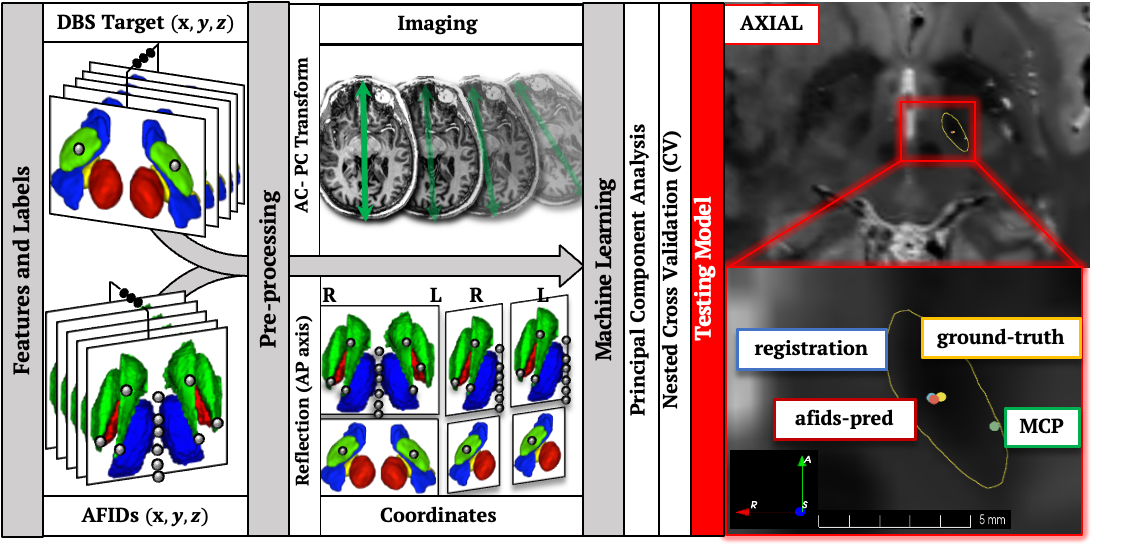
\includegraphics[width=1\linewidth]{figs/ch4_Figure_afidspred.png}
    \caption{Overall workflow for building our machine learning (ML) model to localize the subthalamic nucleus (STN) using anatomical fiducials (AFIDs). Validated AFID coordinates were used as features to predict STN coordinates. All coordinates were anterior commissure (AC) and posterior commissure (PC) aligned. AFID and STN coordinates on the right hemisphere were mirrored to augment data. Principal component analysis (PCA) was performed on coordinate data to capture collinearity. A nested 4-fold cross validation strategy was employed for ML training. Model prediction was validated on various imaging modalities and compared to deformable registration for STN localization.}
    \label{fig:ch4_Figure_afidspred}
\end{figure}
\newpage
\section{Methods}

\subsection{Participants}
We leverage 202 MRI scans on which we have more than 6,500 ground truth anatomical landmarks applied in accordance with a validated annotation protocol \cite{Lau2019-eh} by more than 20 human raters (Table \ref{tab:afidpred_datasets}). Although this data set has been described previously in Chapter \ref{chap:afidsdata}, we divide them below to emphasize their different use cases in this chapter. 

The Stereotactic Neurosurgery (SNSX) dataset. This dataset consists of 61 participants (32 healthy controls and 30 scheduled for DBS). Participants were imaged using a 7T head-only MRI scanner (Siemens Magnetom; Siemens Healthineers, Erlangen, Germany) at the Center for Functional and Metabolic Mapping (CFMM) in Western University (REB: 109045). The MRI sequences used for this study were: 1) 3D T1w MP2RAGE and 2) 3D optimized T2w fast-spin echo (T2 SPACE).

The London Health Sciences Center Parkinson’s Disease (LHSCPD) dataset. This dataset consists of a subset (n = 10) of the same participants as in the SNSX dataset, scheduled to undergo DBS at London Health Sciences Center (LHSC; REB: R-17-156). Participants were imaged using a 1.5T MRI scanner (Signa, 1.5T, General Electric, Milwaukee, Wisconsin, USA). The MRI sequence used in this study was a 3D T1w MP2RAGE with gadolinium contrast (termed “MRI-gad” in subsequent sections).

An openly released 3T and 7T (3T-7T) dataset \cite{Chen2023-cn}, consisting of healthy participants (n = 10) imaged using the following sequences: 1) 3D T1w MP2RAGE and 2) 3D T2 SPACE. Participants are imaged at both 3T and 7T (i.e., test-retest).

A subset of a previously released dataset (afids-data; see Chapter \ref{chap:afidsdata}) dataset, which aggregated landmark annotations (n = 110) on various populations (healthy, abnormal ventricular size, and PD). The participants in this subset are independent of the previously mentioned datasets.

\subsection{Coordinate Data Annotation}
We employ a previously validated protocol for the annotation of anatomical fiducials (AFIDs; \url{https://afids.github.io/afids-protocol}) providing a point-based sampling of multiple brain structures. In this study, we selected a subset of 16 AFIDs (available on \url{https://stereotaxy.afids.io}) described by the protocol that: (1) circumscribe the midbrain and surrounding structures (e.g. DBS targets) and (2) can be localized within 1 mm.

\begin{table}[h!]
\centering
\caption{Various datasets leveraged as part of this study, all of which have curated anatomical landmark annotations.}
\begin{tabularx}{\textwidth}{l l l l l}
\toprule
\textbf{Dataset} & \textbf{Field Strength (T)} & \textbf{Disease (n)} & \textbf{Analysis} \\
\midrule
SNSX* & 7 & HC (32), PD (30) & Training and Testing  \\
LHSCPD & 1.5 (paired SNSX) & PD (10) & Clinical Validation \\
3T-7T* & 3 and 7 (paired) & HC (10) & External Validation  \\
afids-data & 1.5, 3, and 7 & HC (60), PD (40), AD (10) & Landmark Generalization \\
Template & 3 & HC (1) & Landmark Augmentation  \\
\bottomrule
\end{tabularx}

\vspace{1ex}
\raggedright
\footnotesize{
\textbf{HC} = healthy control, \textbf{PD} = Parkinson’s disease, \textbf{AD} = Alzheimer’s disease.\\
* Contains manual human rater curated subthalamic nucleus (STN) segmentations.
}
\label{tab:afidpred_datasets}
\end{table}

\textbf{AFID Annotations:} All annotations were performed in accordance with the AFIDs protocol via 3DSlicer 4.10. Rater placements per AFID were averaged to curate the ground-truth coordinates ($x$, $y$, $z$).

\textbf{STN Annotations:} All annotations were performed via 3DSlicer 4.10 \cite{Fedorov2012-rk} using the smallest configuration of the paint brush (1 mm) and the pencil drawing tool on 7T T2w imaging. Rater segmentations per subject were selected via majority voting (\(>\)50\%) and then collapsed to a center of mass representing the STN centroid, constituting the ground truth STN centroid coordinates ($x$, $y$, $z$).

Each scan was annotated by at least two human raters (see Supplementary section \ref{app:rater_demo_data} for a breakdown of rater demographic data). The ground truth coordinates were quality controlled (QC) by three raters (AT, JZ, and EC). We provide example QC files (Supplementary Section \ref{app:qualitycontrol}) with accompanying code and ground truth coordinates (*.fcsv) used in this work on: \url{https://github.com/afids/afids-pred}.

\subsection{Coordinate Data Processing}
An AC-PC alignment was performed followed by centering coordinates at the mid-commissural point (MCP; defined as the midpoint between AC and PC). Coordinates on the left hemisphere were reflected to the right by inverting the sign of the x-coordinate after AC-PC transformation and MCP centering. Thus, each participant constituted two augmented examples. Preliminary analysis using training data was conducted to investigate correlations across coordinates to inform ML. Subsequently, principal component analysis (PCA) was performed on concatenated x, y, z coordinates. Top principal components (PCs) capturing 99\% of the variance were retained for subsequent ML model training.

\subsection{Data Split and Machine Learning}\label{chap:afidspredML}
AFID and STN coordinate data of participants from the SNSX dataset were used for ML training. Ten participants from the SNSX dataset were assigned to a reserved testing dataset used solely to report the accuracy of our model. These participants were also the same ones from the LHSCPD dataset, enabling evaluation of our model on clinical quality 1.5T MRI-gad scans. Finally, the 3T-7T dataset was used for external validation to report prediction accuracy at 3T and 7T MRI.

To explore the trade-off between model simplicity and complexity, we evaluated two ML algorithms: (1) \textit{Ridge Regression} \cite{Hoerl1970-so}, a linear model with built-in regularization, and (2) \textit{Extreme Gradient Boosting} (XGBoost; \cite{Friedman2001-hp}), an ensemble-based method capable of modeling non-linear relationships. 

ML models were trained via a nested cross-validation (CV) strategy to tune hyperparameters and evaluate performance (scikit-learn; \cite{Pedregosa2012-ab}). The outer CV loop involved a 4-fold split of all training data for statistically evaluating the two ML models, and the inner CV loop involved a 3-fold split CV strategy for tuning hyperparameters. All the folds were curated such that for a given training example (i.e., participant) the left and right hemisphere target labels (e.g., STN) were grouped together. This prevented a scenario where the left and right labels appear separately across training and testing to avoid data leakage. Furthermore, group based preprocessing (i.e., PCA) was performed independently within each fold to prevent leakage across folds. Final model accuracy was reported on the four testing sets curated by the outer CV loops. We compute the x, y, z mean squared error (MSE) and Euclidean distance (ED) to evaluate models. See Figure~\ref{fig:ch4_Figure_afidspred} for an end-to-end abstraction of our methodology.

\subsection{Model Robustness, Generalizability, and Comparative Evaluation}

\textbf{Generalization to Other Imaging Modalities.} To investigate model accuracy on clinical-grade imaging, STN coordinate predictions on 1.5-T MRI-gad scans were statistically compared to paired ground-truth counterpart 7-T MRI-nogad scans. To further demonstrate robustness across research-grade imaging and external data, we also evaluated model predictions on the 3T–7T dataset. Statistical comparisons were in AC-PC space and two independent Wilcoxon signed-rank tests were performed across $x$,$y$,$z$ MSE and ED with Bonferroni correction ($\alpha = 0.05 / 4$).

\textbf{Benchmarking.} We perform statistical comparisons between our model and deformable registration for STN localization using our 1.5T MRI-gad dataset (i.e., LHSCPD) and paired 7T-MRI counterpart (i.e., SNSXPD). The Distal atlas segmentations in MNI space \cite{Chakravarty2006-ln, Ewert2018-bn} were warped to native space using presets from a nonlinear deformation framework validated via 11,000 non-linear warps across more than 100 subjects \cite{Ewert2019-cc}. We apply this framework as implemented in Lead-DBS software (v.3.1; \cite{Neudorfer2023-wd}). Groups were compared using a signed-Wilcoxon Rank Test.

\textbf{Robustness to Annotation Variability.} To investigate model dependency on accurate localization, we make use of 38 independent AFID protocol applications in a common space (i.e., MNI) and evaluate STN prediction accuracy across these trials. For this analysis, the AFID protocol was applied independently by 10 human raters. 

\textbf{Generalizability to Other Brain Landmarks.} To investigate the generalizability of our framework to other brain landmarks, we iteratively drop each brainstem AFID (i.e., leave-one-AFID out) and predict it using the other AFIDs. This analysis was conducted using all the datasets (i.e., n = 202) for nine AFIDs and employed the same nested-cross validation approach described in section \ref{chap:afidspredML}.

\subsection{Model Deployment}
Building on the previous open software infrastructure of the AFID project, we deploy our model on a website (\url{https://stereotaxy.afids.io}). This enables users to upload their AFID placements as specified by our protocol and receive STN coordinate predictions alongside an AC-PC transformation matrix. Additionally, we also deploy our STN prediction model within a larger suite of coordiante-based tools (i.e., \texttt{AutoAFIDs}; see Chapter \ref{chap:AutoAFIDs}) which automatically localizes AFIDs from MRI volume. Details about running the end-to-end workflow (i.e., image to DBS target) is presented in Supplementary content \ref{app:stereotaxyautoafids}. For subsequent sections, we report the results and discuss them independently of \texttt{AutoAFIDs} for completeness. 

\section{Results}

\subsection{Rater Curated Data}
The localization error across all AFID placements and datasets was 0.84~$\pm$~0.31~mm. The inter-rater STN segmentation overlap was 0.78~$\pm$~0.03, measured using the Dice similarity coefficient. There was no statistical difference between right and left hemisphere STN segmentations, thus they were combined in subsequent descriptive summaries. The average volumes of the STN for the healthy control (HC) and Parkinson’s disease (PD) cohorts were 136.56~$\pm$~16.24~mm\textsuperscript{3} and 128.03~$\pm$~29.67~mm\textsuperscript{3}, respectively ($p = 0.047$; Mann–Whitney U test). The average x, y, z STN coordinates in MCP space for the HC and PD cohorts were: 10.18, -0.92, -3.27 and 10.14, -0.88, -3.61, respectively (x: $p = 0.93$, y: $p = 0.91$, z: $p = 0.002$; Mann–Whitney U test). Only the z-coordinate was statistically significant after Bonferroni correction ($\alpha = 0.05/4$).

\subsection{Preliminary Analysis and Principal Component Analysis}
Pairwise correlations were computed among the x, y, and z coordinates of 16 AFIDs (48 features total) across training data (see Figure~\ref{fig:ch4_Figure_PCA}a). Principal component analysis (PCA) was employed to reduce the dimensionality of features used for ML model training. The top 23 principal components (PCs) captured 99\% of the variation in the data (see Figure~\ref{fig:ch4_Figure_PCA}b) and were chosen for subsequent analysis. Further exploration of AFID contributions to PCs revealed relatively broad AFID contributions (see Figure~\ref{fig:ch4_Figure_PCA}c). Strong linear associations between AFID coordinates and STN x, y, and z coordinates were observed (Pearson’s r = -0.38–0.54) in the training data (see Figure~\ref{fig:ch4_Figure_stncor}), supporting the use of a linear regression framework.

\begin{figure}[hbt!]
    \centering
    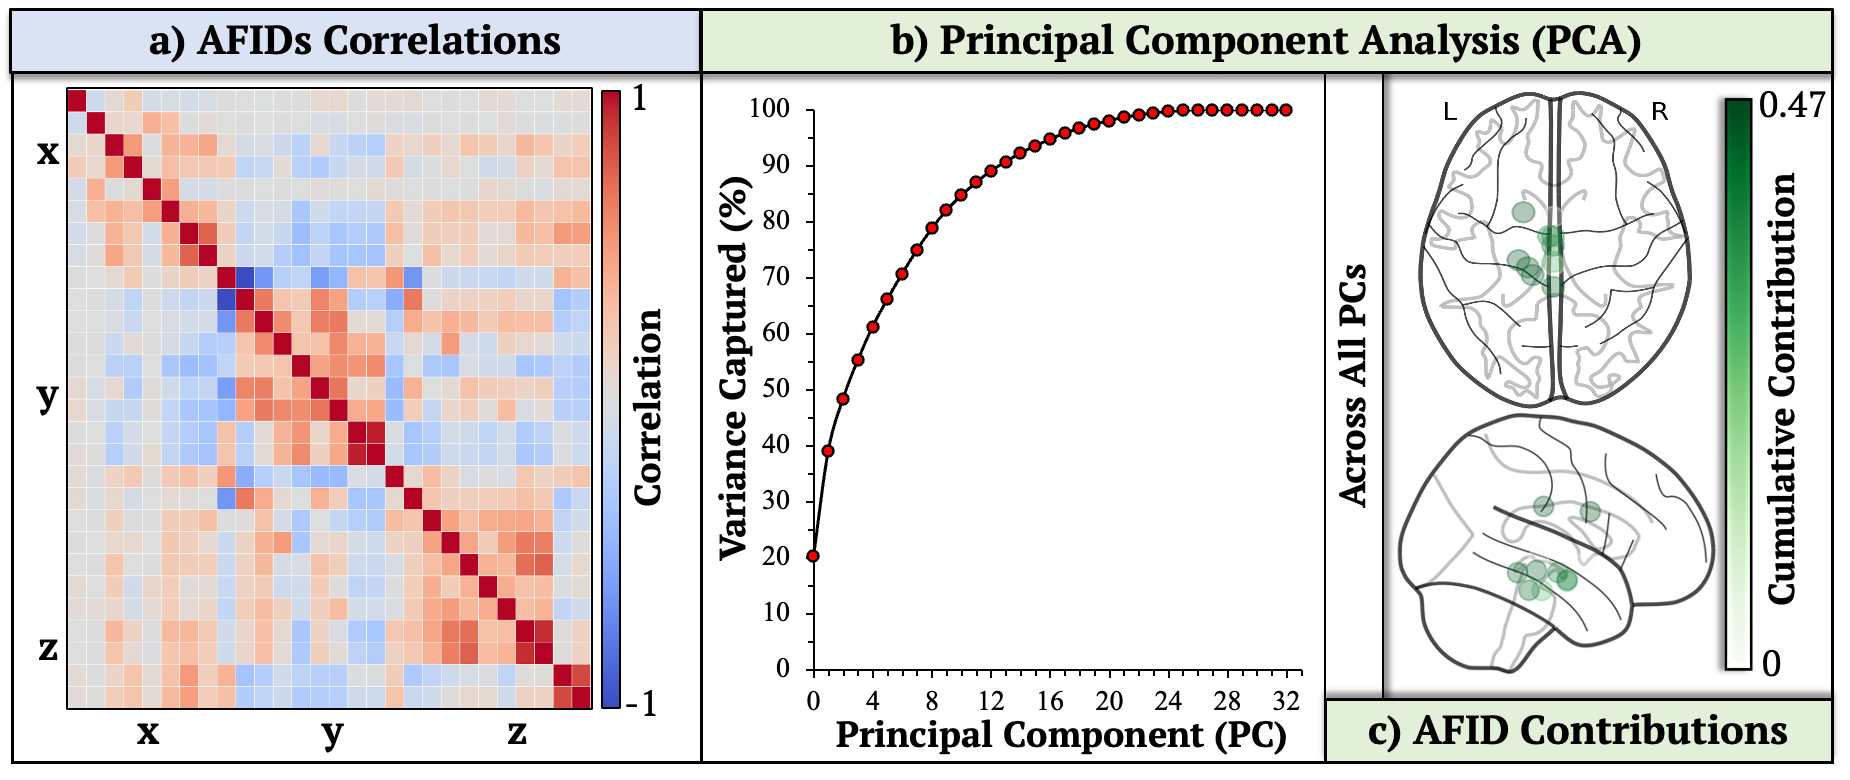
\includegraphics[width=1\linewidth]{figs/ch4_Figure_PCA.png}
    \caption{Correlation and visual representation of landmarks and Principal Component Analysis (PCA). a) Correlation matrix between the x, y, and z coordinates of anatomical fiducials (AFIDs) chosen to build the machine learning model, post anterior and posterior commissure (AC-PC) transformation and mid-commissural point (MCP) centering. b) Cumulative explained variance plot as a function of principal components (~99\% of the variation with 24 components). c) Shows the weight contribution of each AFID’s x, y, and z coordinates to all principal components.}
    \label{fig:ch4_Figure_PCA}
\end{figure}

\subsection{Machine Learning Model Performance}
\textbf{Model Training:} A multi-output paradigm using nested CV was used to train a ridge regressor and an XGBRegressor. ED computed on the outer CV folds was compared using a Wilcoxon signed-rank test, and the ridge regressor statistically outperformed the XGBRegressor ($\alpha = 0.05$, $p < 0.01$), supporting its use as the final model for predicting STN coordinates.

\begin{figure}[hbt!]
    \centering
    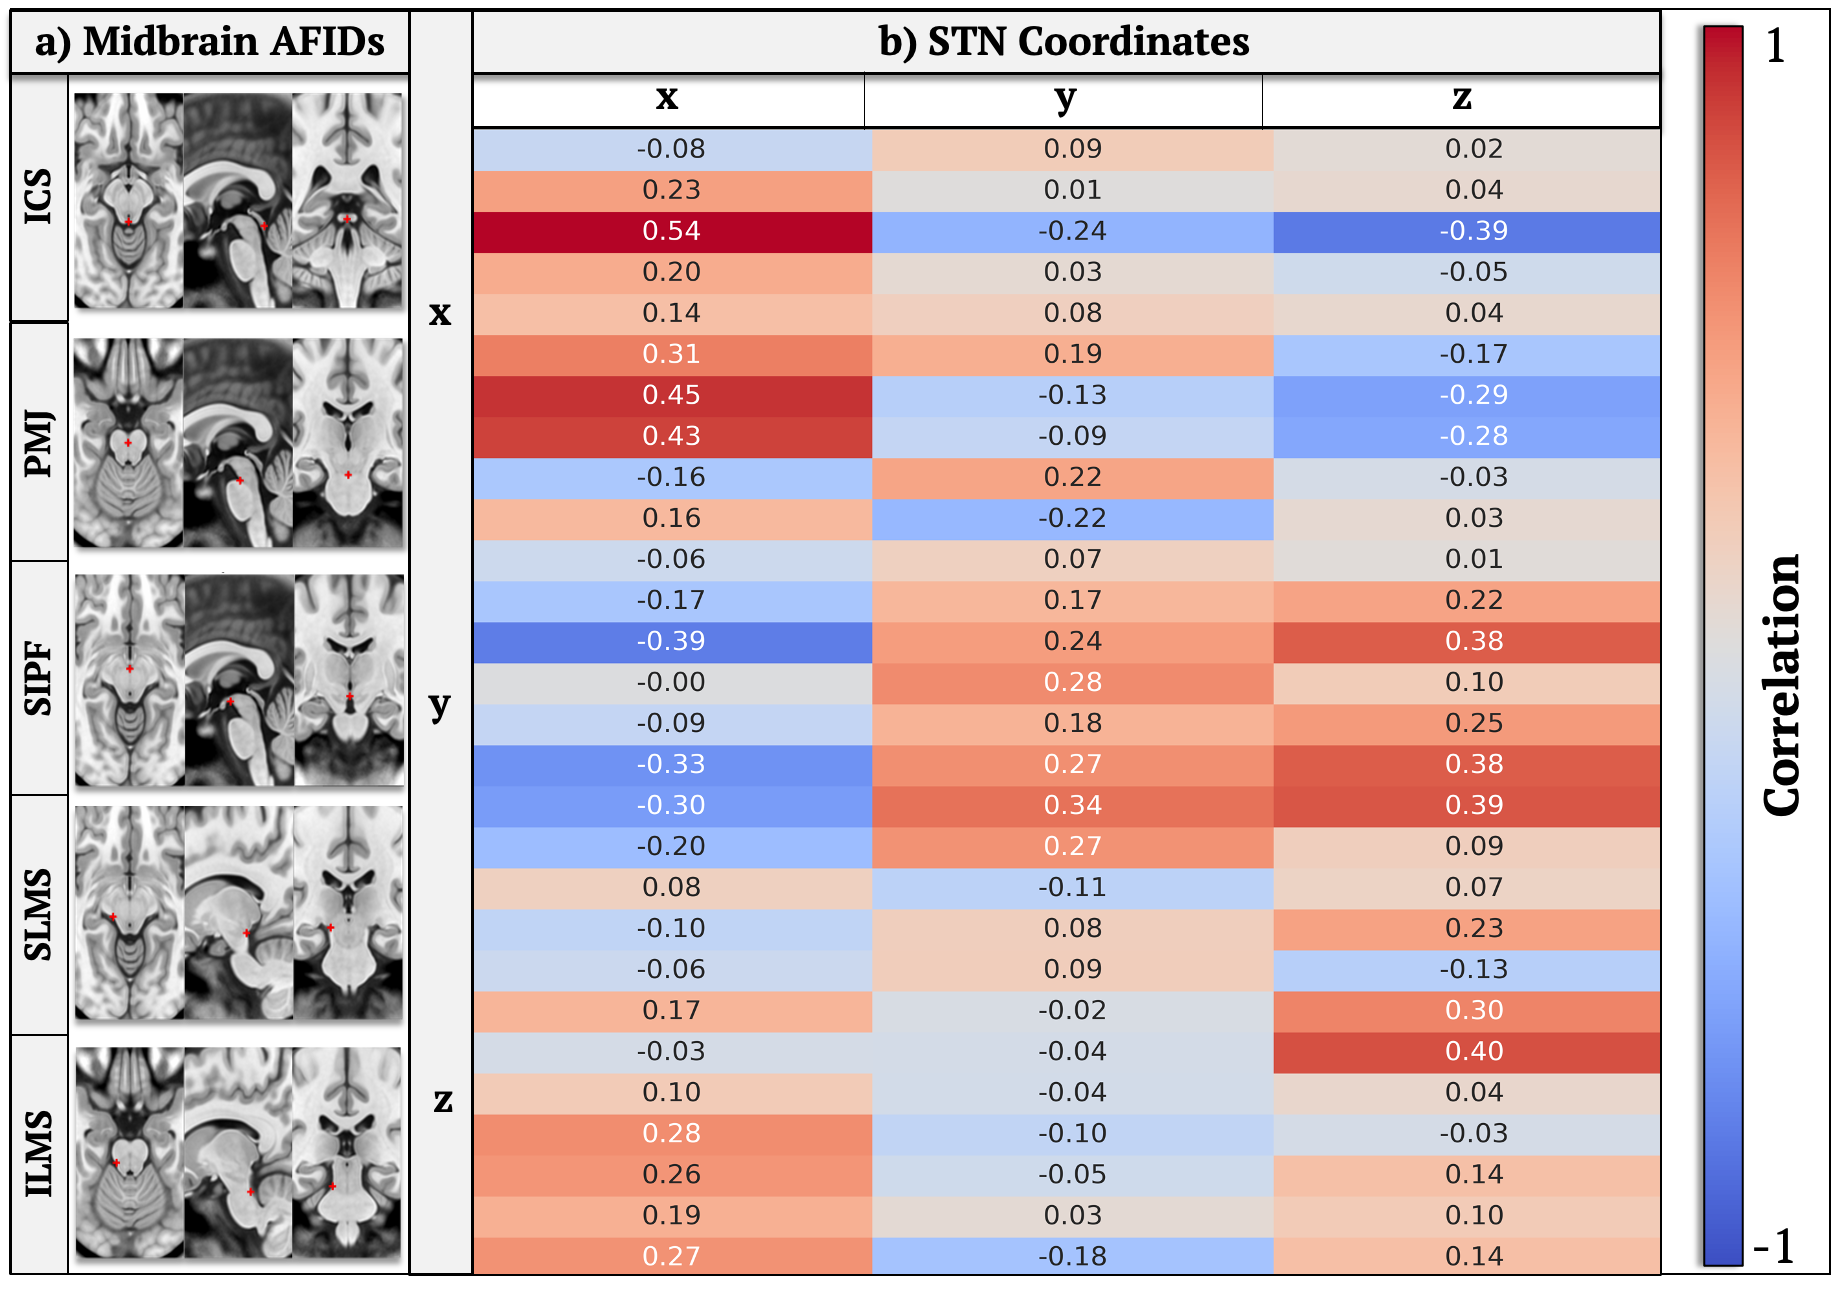
\includegraphics[width=1\linewidth]{figs/ch4_Figure_stncor.png}
    \caption{Correlation matrix of anatomical fiducials (AFIDs) and subthalamic nucleus (STN) coordinates. a) shows a subset of five AFIDs in the three cardinal planes which closely circumscribe the STN for anatomical context. b) Strong linear associations between x,y,z components of AFIDs and x,y,z dimensions of STN center of mass. }
    \label{fig:ch4_Figure_stncor}
\end{figure}

\textbf{Model Testing:} The average x, y, z mean squared errors (MSE) across all testing data (40 STNs) were: 0.45~$\pm$~0.56~mm, 0.66~$\pm$~0.79~mm, and 0.48~$\pm$~0.58~mm, respectively. The overall median ED error was 1.20~$\pm$~0.44~mm (IQR: 0.84–1.52). See Table~\ref{tab:performance_metrics} for a more granular breakdown of results.

\begin{table}[htbp]
\centering
\small
\caption{Performance of the final machine learning model across test datasets. Values are reported as Median ± Standard Deviation [Interquartile Range] for each dataset. Metrics include mean squared error (MSE) in the $x$, $y$, and $z$ directions, and Euclidean distance (ED).}
\label{tab:performance_metrics}
\begin{tabularx}{\textwidth}{lXXXX}
\toprule
\textbf{Dataset} & \textbf{MSE (x)} & \textbf{MSE (y)} & \textbf{MSE (z)} & \textbf{ED} \\
\midrule

\textbf{Testing Data (SNSX)} & 
0.48 ± 0.48 [0.22–0.88] & 
0.30 ± 0.77 [0.08–0.76] & 
0.43 ± 0.38 [0.03–0.72] & 
1.19 ± 0.37 [0.98–1.50] \\

\textbf{Clinical Validation (LHSCPD)} & 
0.24 ± 0.58 [0.09–0.68] & 
0.80 ± 0.87 [0.08–0.93] & 
0.57 ± 0.58 [0.11–0.79] & 
1.32 ± 0.42 [1.07–1.58] \\

% \textit{p}-value (SNSX vs LHSCPD) & 
% 0.13 (ns) & 
% 0.09 (ns) & 
% 0.11 (ns) & 
% 0.12 (ns) \\

\cmidrule(l){1-5}

\textbf{External Validation (3T)} & 
0.10 ± 0.57 [0.05–0.44] & 
0.43 ± 0.76 [0.06–1.30] & 
0.07 ± 0.78 [0.02–0.65] & 
1.20 ± 0.49 [0.80–1.49] \\

\textbf{External Validation (7T)} & 
0.07 ± 0.60 [0.02–0.27] & 
0.26 ± 0.78 [0.04–0.93] & 
0.17 ± 0.57 [0.03–0.49] & 
1.08 ± 0.48 [0.70–1.40] \\

% \textit{p}-value (3T vs 7T) & 
% 0.21 (ns) & 
% 0.31 (ns) & 
% 0.52 (ns) & 
% 0.15 (ns) \\

\bottomrule
\end{tabularx}
\end{table}

\subsection{Model Generalizability and Comparisons}

\textbf{Validation across Other Imaging Modalities:} We evaluated model performance across different imaging modalities by analyzing paired datasets acquired at various field strengths (see Figure~\ref{fig:ch4_Figure_errs}). Ten participants with both 1.5T MRI-gad (LHSCPD) and 7T MRI-nogad (SNSX), as well as ten participants with both 3T and 7T MRI (3T-7T), were included (see Section \ref{chap:afidspredML}). Wilcoxon signed-rank test with Bonferroni correction ($\alpha = 0.05/4$) revealed no significant differences in x, y, z MSE and ED across the two paired imaging modalities.

\begin{figure}[hbt!]
    \centering
    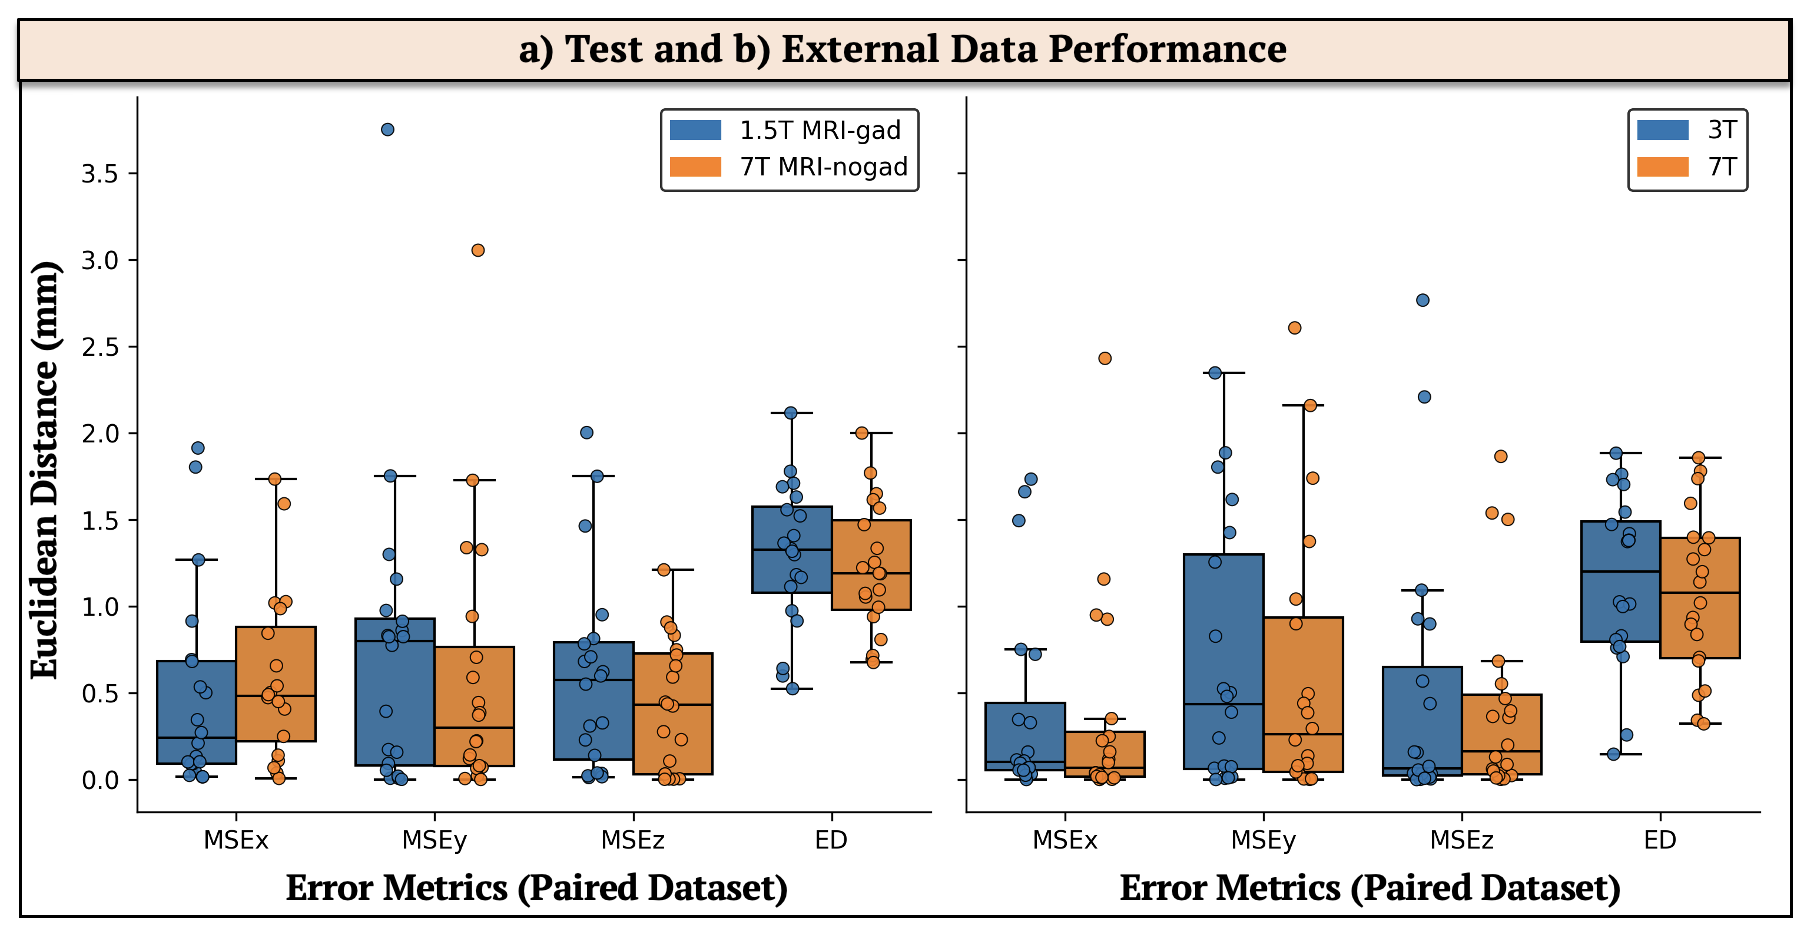
\includegraphics[width=1\linewidth]{figs/ch4_Figure_errs2.png}
    \caption{Model Performance on MRI modalities of Test-retest Datasets. a) shows model performance on 1.5T MRI with gadolinium (gad) and 7T MRI without gadolinium. b) shows model performance on 3T and 7T MRI. p \(>\) 0.1 across all axes and Euclidean distance. }
    \label{fig:ch4_Figure_errs}
\end{figure}

\textbf{Model Comparison and Performance Benchmarking:} We benchmarked our model against deformable registration (see Figure~\ref{fig:ch4_Figure_bench}a). On 1.5T MRI-gad scans, our model statistically outperformed registration ($p < 0.001$). Conversely, on multispectral 7T MRI-nogad data (i.e., registration warps computed using both T1 and T2 imaging), no significant difference in performance was observed between registration and our model ($p > 0.1$).

\begin{figure}[hbt!]
    \centering
    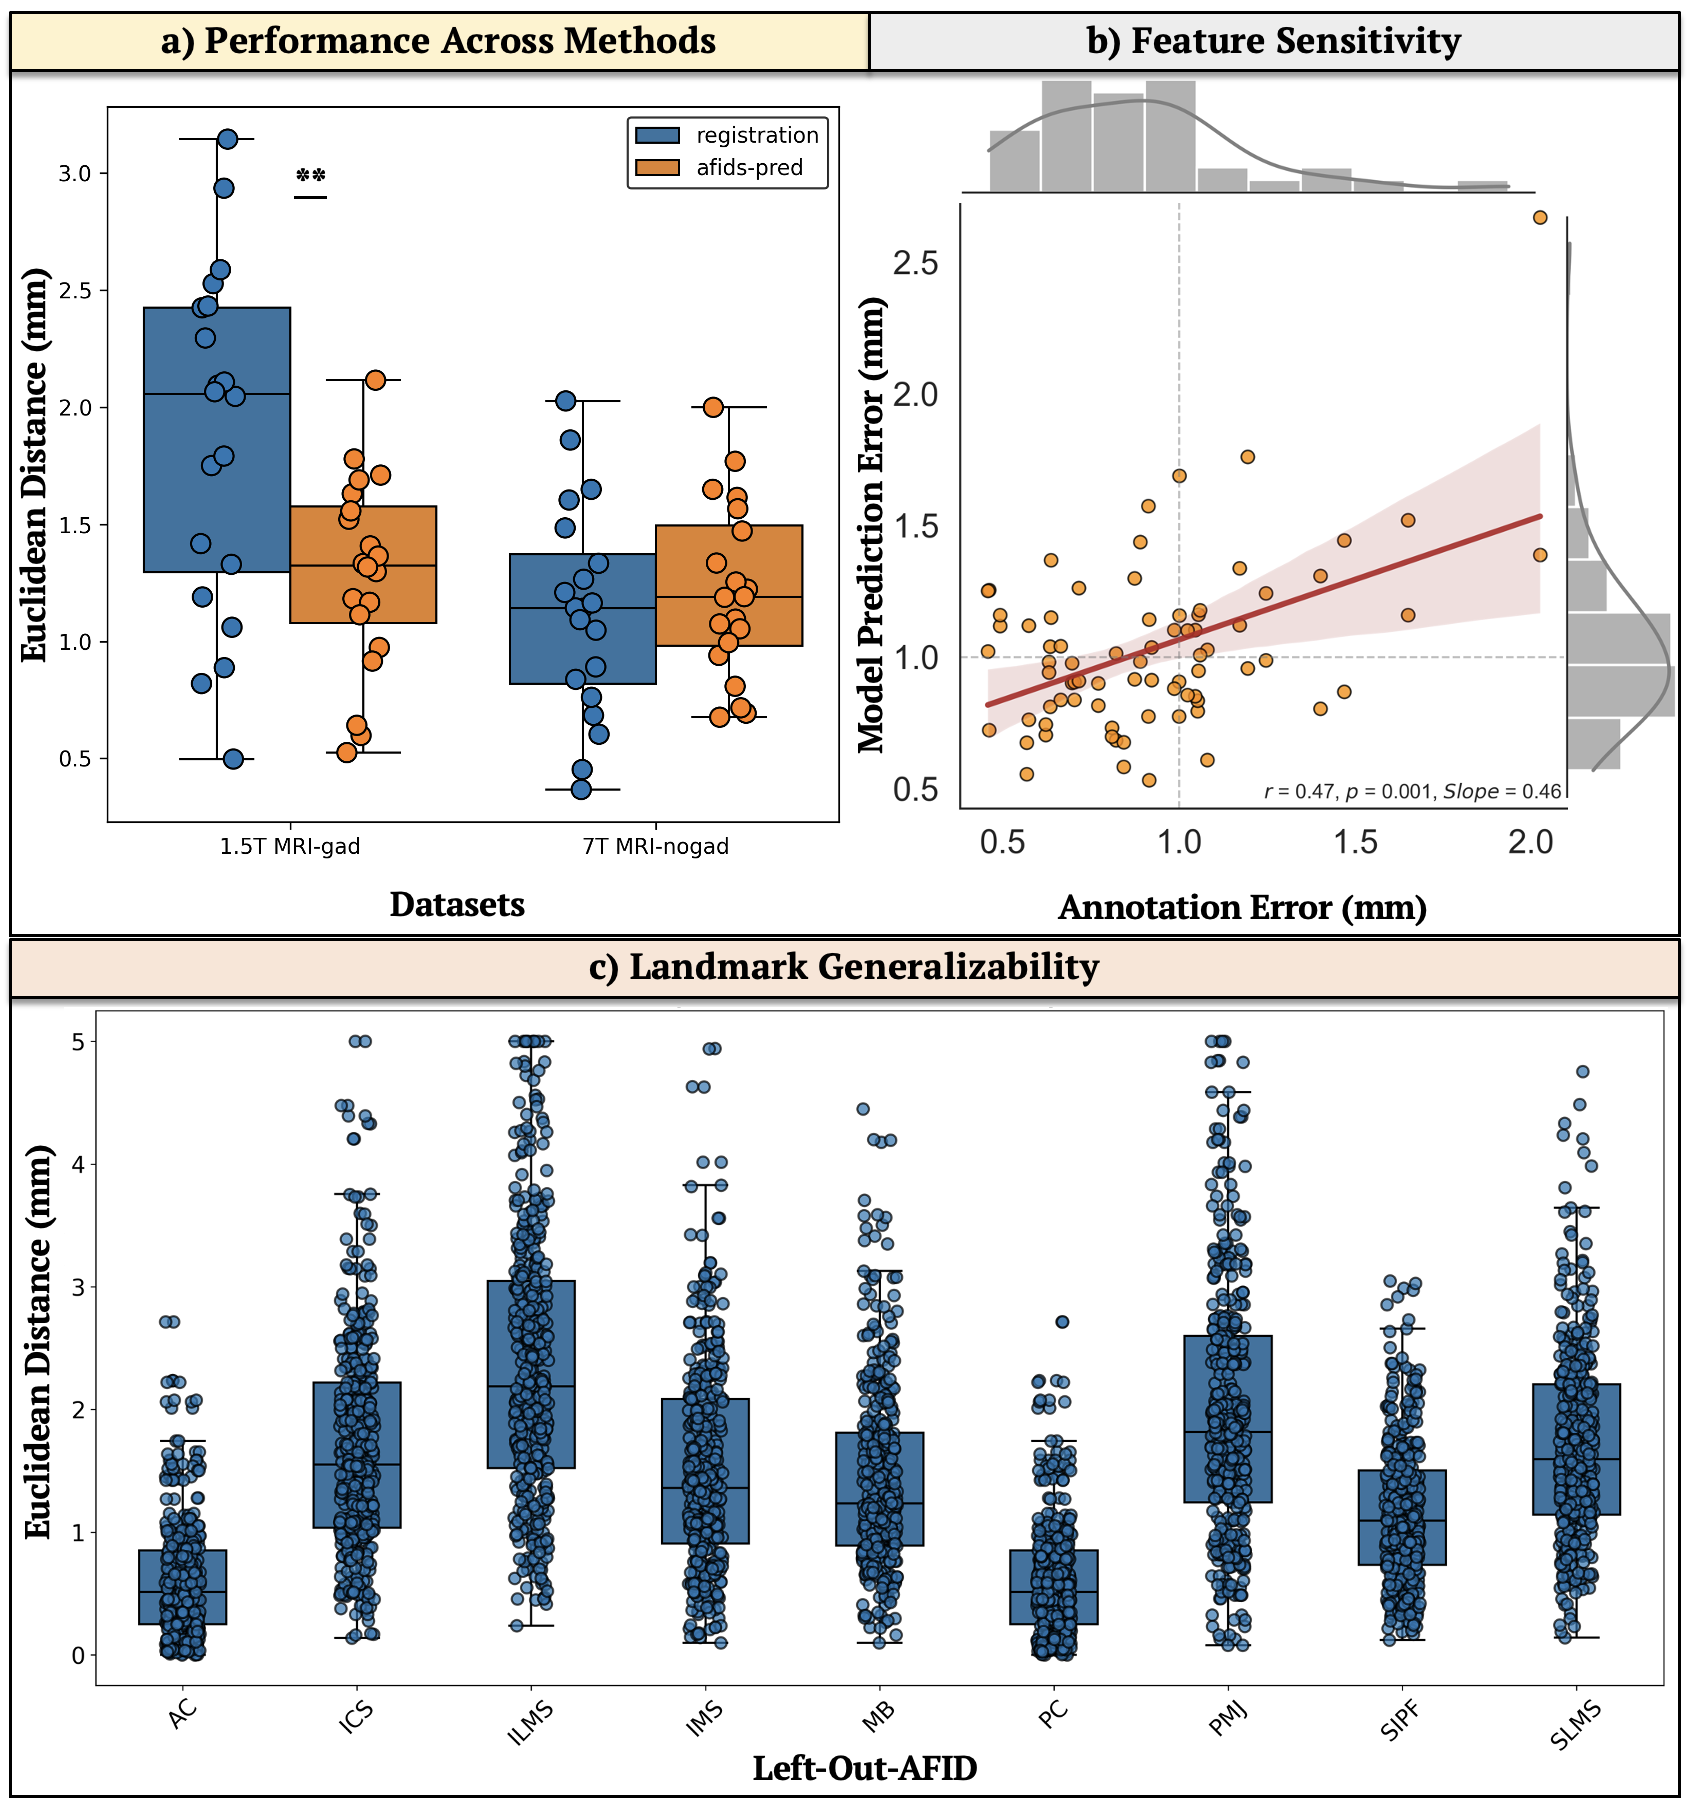
\includegraphics[width=1\linewidth]{figs/ch4_Figure_bench2.png}
    \caption{Model Benchmarking. a) Our model outperformed registration on the 1.5T MRI-gad dataset (p \(<\) 0.001) and performed just as well when using multispectral 7T MRI data (p \(>\) 0.1). b) AFID localization error was moderately linearly correlated with model performance (Pearson r = 0.47). c) Generalization to nine other midbrain landmarks.}
    \label{fig:ch4_Figure_bench}
\end{figure}

\textbf{Feature Importance and Augmentation:} To assess the influence of landmark annotation error on model performance, we examined the relationship between rater AFID localization error and ML model prediction error. A moderate correlation was observed (Pearson $r = 0.47$; $p < 0.01$), see Figure~\ref{fig:ch4_Figure_bench}b).
\newpage
\textbf{Generalizability to Other Brain Landmarks:} To assess the broader applicability of our framework, we extended the localization approach to nine additional midbrain landmarks (see Figure~\ref{fig:ch4_Figure_bench}c). The model maintained high accuracy across all these structures, achieving a median ED of 1.27~$\pm$~0.96~mm (IQR: 0.73–2.00).

\subsection{Clinical Use Cases}
We evaluated the functionality of our website using two illustrative DBS cases from our center (see Figure~\ref{fig:ch4_Figure_clincase}). In \textbf{Case 1}, we independently applied our framework to multimodal imaging data. The predictions were consistently within 1 mm across the following modalities: (1) 1.5-T MRI-gad, (2) 7-T T1w MRI, (3) 7T T2w MRI, and (4) contrast-enhanced CT. In \textbf{Case 2}, we demonstrated the application of our model to post-operative MRI from a DBS re-implantation case, highlighting its robustness in the presence of electrode artifacts that may complicate image-based localization methods.

\section{Discussion}
We demonstrated that coordinates of predefined brain landmarks can be leveraged to predict the coordinates of other surrounding brain regions with millimetric accuracy. By employing a coordinate-to-coordinate ML framework, our model is agnostic to MRI modality and resolution. Furthermore, we demonstrated that our model outperforms conventional methods when using challenging clinical-grade scans (e.g., 1.5-T MRI-gad) and performs just as well when using multispectral research-grade scans (i.e., 7-T MRI). Finally, we packaged this model in the form of a website, enabling its use in clinical and neuroimaging contexts.

\subsection{Rater Curated Data}
\textbf{AFID Annotations.} Previous AFID validation studies demonstrated millimetric localization in healthy \cite{Lau2019-eh} and clinical populations \cite{Abbass2022-lf}. The subset of 16 AFIDs in our ML framework were selected for their spatial proximity to the STN, sampling the morphology of the midbrain region. Although the complete AFIDs protocol (i.e., 32 AFIDs) typically requires 20–40 minutes following rater training, we anticipate a substantial reduction in annotation time due to the reduced number of AFIDs used here. To facilitate reproducibility and completeness, we provide a website embedded protocol tailored to the 16 AFIDs used in this work: \url{https://stereotaxy.afids.io}.
\begin{figure}[hbt!]
    \centering
    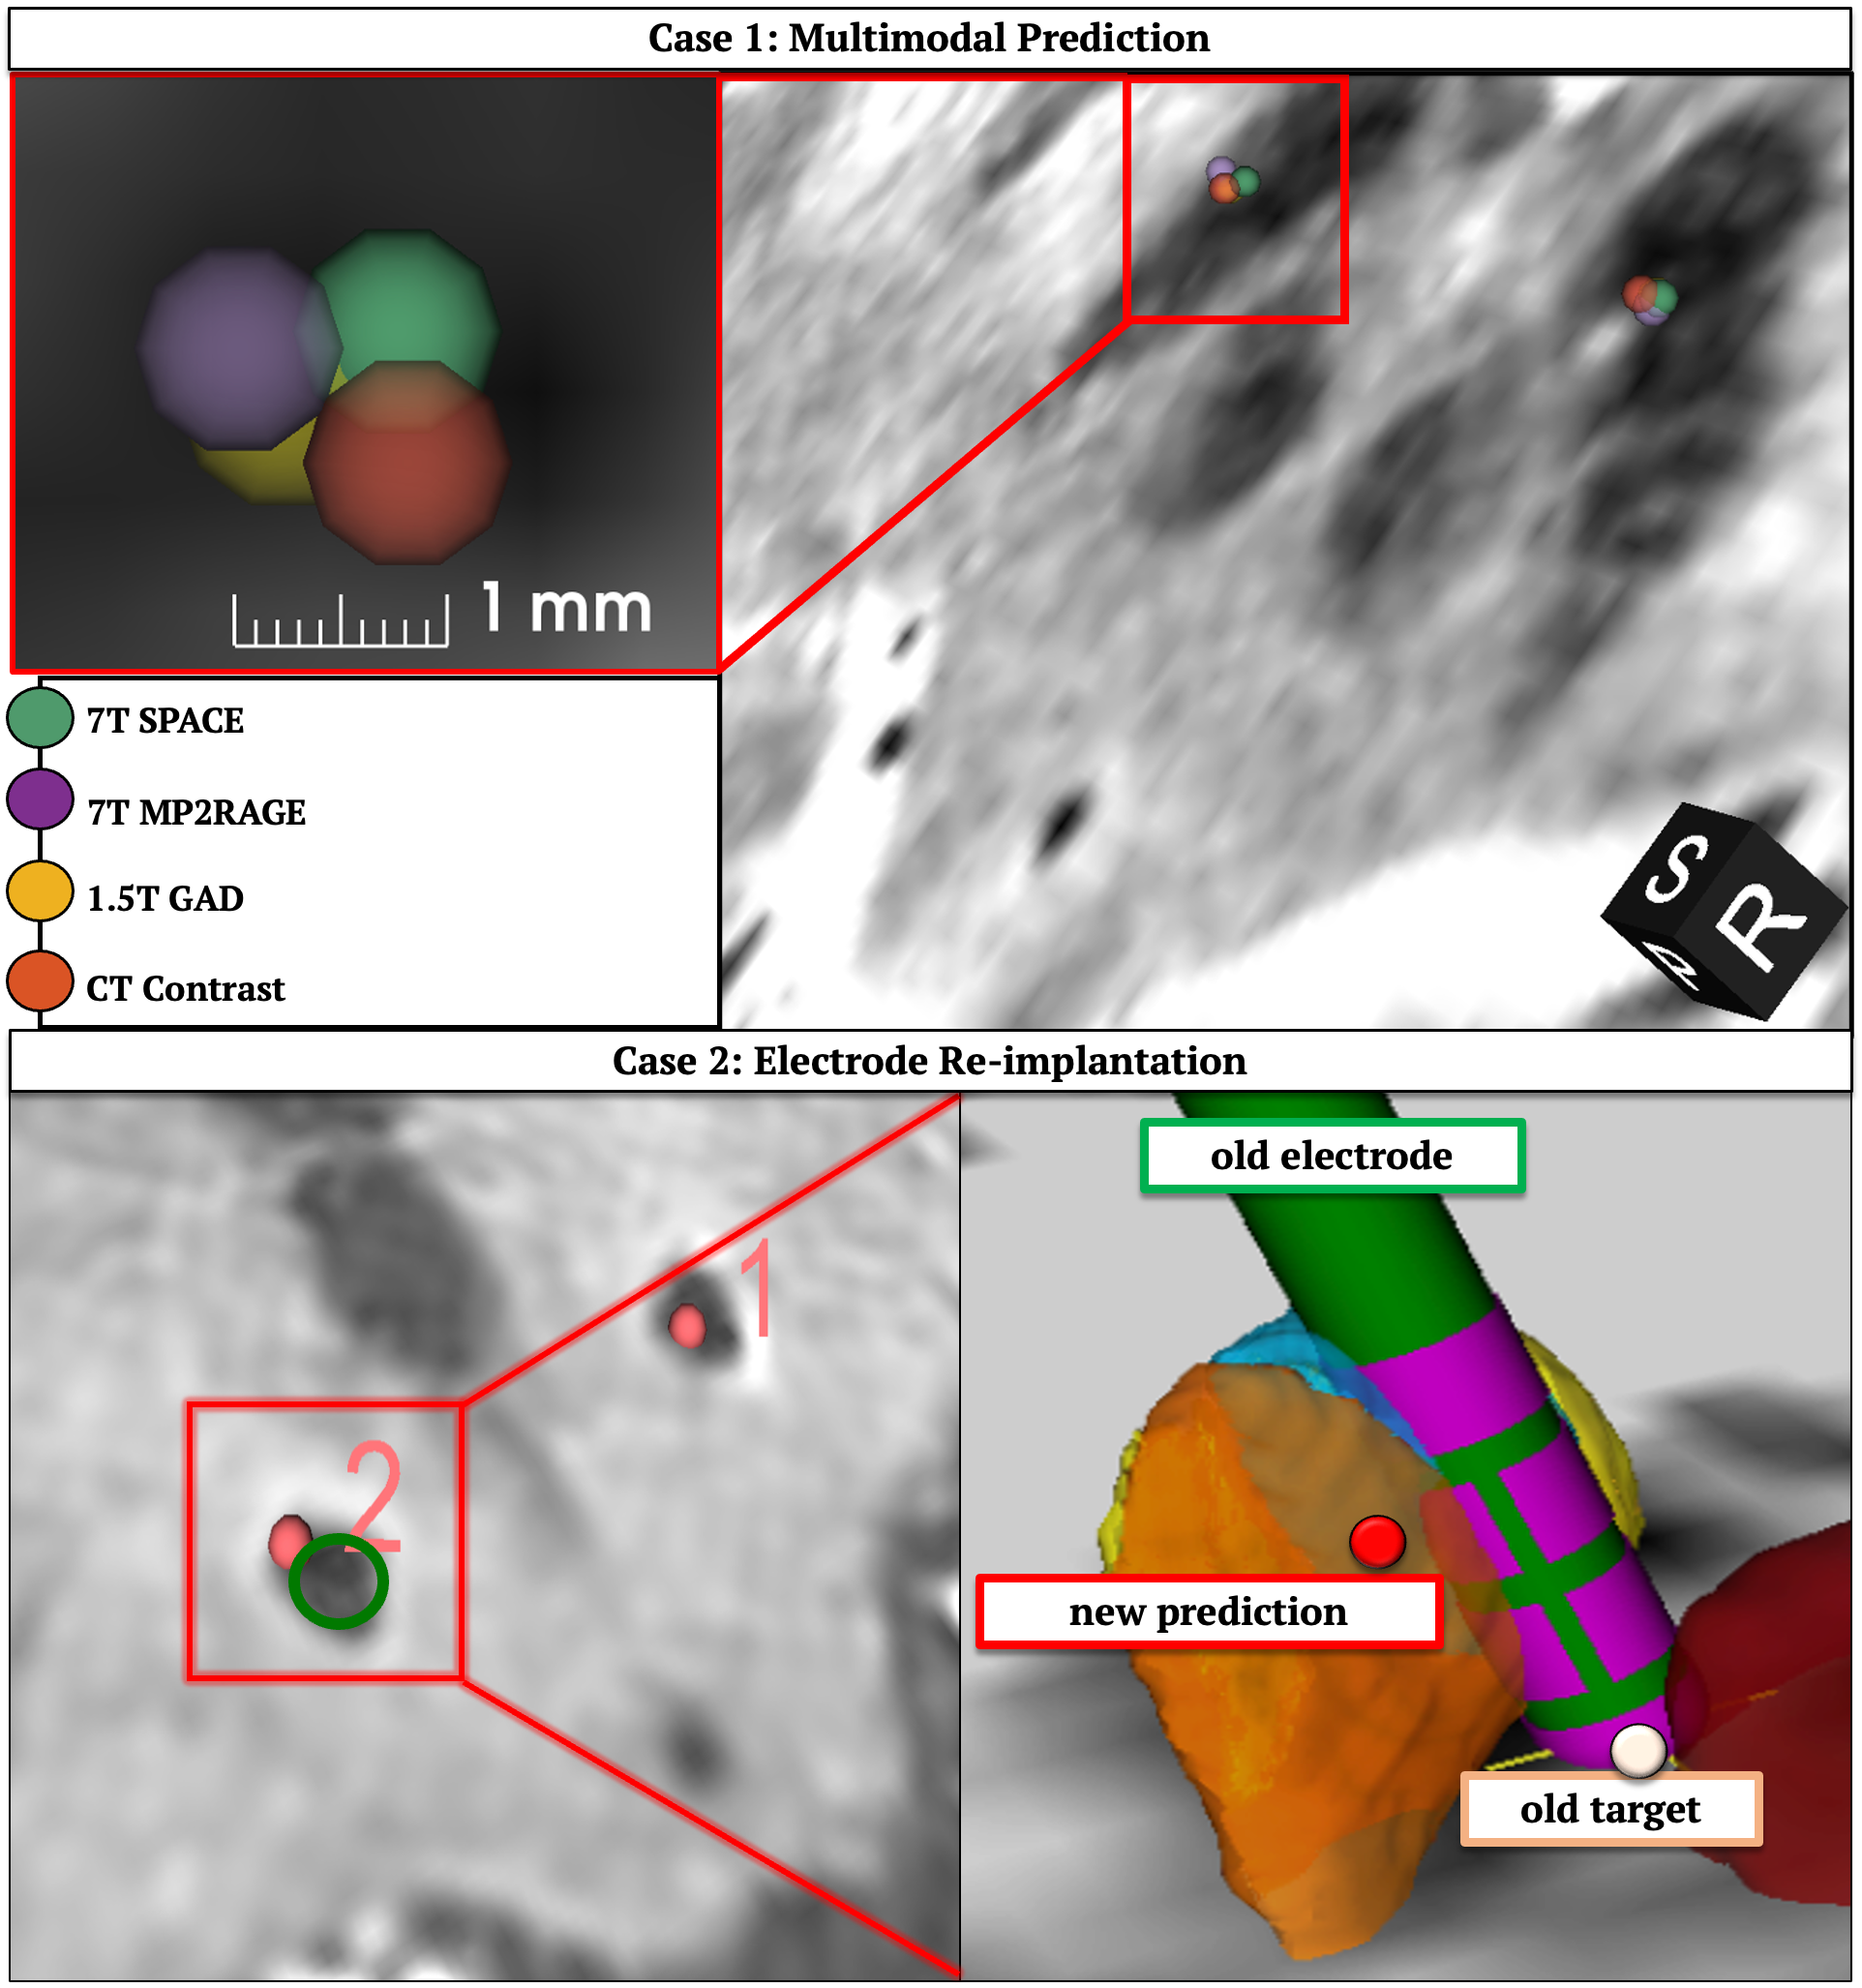
\includegraphics[width=1\linewidth]{figs/ch4_Figure_clincase.png}
    \caption{Clinical use cases. Case 1) Model prediction on multimodal neuroimaging data is within 1 mm of ground truth location as defined by expert raters on 7T-T2w MRI. All comparisons are made in anterior and posterior commissure space. Case 2) Model performance during a deep brain stimulation electrode re-implantation case using the postoperative MRI scan. Acquiring high-resolution imaging was not feasible due to the presence of electrodes}
    \label{fig:ch4_Figure_clincase}
\end{figure}

\newpage
\textbf{STN Annotations.} Inter-rater agreement for STN segmentation was strong, with a Dice similarity coefficient of \( 0.78 \pm 0.03 \). This is consistent with prior manual segmentation studies of the STN and nearby subcortical structures \cite{Camlidag2014-za,Miller2023-ct}. Prior work also highlighted that no statistically significant differences were found between left and right STN annotations \cite{Duchin2018-sv, Miller2023-ct}, justifying their combination in subsequent analyses. On average, the STN volume was reduced in the PD cohort relative to controls (\( 128.03 \pm 29.67 \text{ mm}^3 \) and \( 136.56 \pm 16.24 \text{ mm}^3 \), \( p = 0.047 \)). However, this volume difference did not remain statistically significant after Bonferroni correction. Prior studies reported conflicting findings, with some showing no significant difference in STN volume between PD and HC \cite{Alkemade2017-tt, Camlidag2014-za}, while others showing a reduction in the PD cohort \cite{Colpan2010-up, Patriat2020-cm}. We believe a meta-analytic approach is needed for more conclusive findings. Analysis of STN coordinates relative to the MCP revealed a significant inferior shift (i.e., z-axis) in PD patients compared to controls (\( p = 0.002 \)). This finding may support prior work reporting region-specific morphological changes associated with PD \cite{Kaya2019-wa}. Interestingly, previous work comparing STN coordinates between PD and essential tremor patients reported no significant differences \cite{Duchin2018-sv}; however, essential tremor may not serve as an appropriate baseline for comparison.

\subsection{Preliminary Analysis and PCA}
Our analysis demonstrates that brainstem AFIDs exhibit strong internal spatial correlations, consistent with prior reports of geometrical regularity in this region \cite{Perera2024-lq}. Structures such as the superior lateral mesencephalic sulcus (SLMS), superior interpeduncular fossa (SIPF), and mammillary bodies (MB) were tightly coupled along shared axes, suggesting conserved spatial organization may be driven by developmental and structural constraints \cite{Parraga2016-bl}. PCA supported this anatomical consistency, with the top five components capturing over 90\% of the variance in AFID coordinates. This high redundancy enables efficient dimensionality reduction for downstream ML applications, preserving anatomical information while reducing model complexity. Importantly, variance was broadly distributed across AFIDs rather than dominated by a few landmarks, reflecting coordinated spatial variation across regions. When correlating AFIDs with STN coordinates, SLMS ranked among the top predictors for all axes (\( r = 0.28\text{-}0.54 \)). The MB and SIPF also demonstrated strong associations (MB: \( r = 0.32\text{--}0.40 \); SIPF: \( r = 0.38\text{--}0.39 \)), highlighting the predictive value of midbrain and diencephalic landmarks. Taken together, these results support a coordinate-based localization approach, leveraging anatomical relationships to infer the position of brain targets.

\subsection{ML Model Performance}
Our model achieved a median localization error of \( 1.20 \pm 0.44\text{mm} \) (IQR: \( 0.84 - 1.52 \)) across all testing data. This performance is comparable to the localization variability of AFIDs themselves, previously reported to range from \( 0.36 \) to \( 1.68 \text{ mm} \) \cite{Lau2019-eh}. For context, a recent study reported an inter-rater centroid localization error of \( 1.90 \pm 1.07 \text{ mm} \) between two expert annotators \cite{Miller2023-ct}. A related coordinate-to-coordinate framework \cite{Engelhardt2021-zd} achieved a mean error of \( 1.33 \pm 1.64 \text{ mm} \); however, direct comparison is limited, as their target was the active contact of a DBS electrode rather than an anatomical structure. Notably, \cite{Guo2007-nf} benchmarked six STN targeting methods and found that a combined anatomical and functional approach yielded a localization error of \( 1.70 \pm 0.7 \text{ mm} \). Clinically, errors under \( 2 \text{ mm} \) are generally acceptable \cite{Kremer2023-if}, particularly when considering the typical stimulation volume of a DBS electrode.

\subsection{Model Generalizability and Comparisons}
\textbf{Validation Across Other Imaging Modalities.} This analysis was enabled by the use of paired datasets, allowing for direct comparison of predictions across modalities within the same subjects. Our framework’s accuracy was maintained across a range of imaging modalities. These findings align with prior work from our group, which established the feasibility of accurately localizing AFIDs across research-grade and clinical-grade MRI scans \cite{Taha2023-gd}. Importantly, comparisons were conducted in AC-PC space, which assumes that independent AFID placements across paired modalities result in equivalent transforms. This approach was necessary due to the lack of ground truth STN segmentations in both the 1.5-T MRI-gad and 3-T MRI datasets. Despite this potential source of error, our results revealed no statistically significant differences in predicted coordinates.

\textbf{Model Comparison and Performance Benchmarking.} We used the default registration pipeline in Lead-DBS to transform images from stereotactic space to native space. This pipeline employs rigorously optimized parameters \cite{Ewert2019-cc,Schonecker2009-xj} for diffeomorphic registration from Advanced Normalization Tools \cite{Avants2008-ek}. It also incorporates subcortical masks to refine deformation fields, enhancing registration accuracy at the STN and surrounding subcortical structures \cite{Ewert2019-cc, Schonecker2009-xj}. Our model statistically outperformed registration when using 1.5-T MRI-gad scans. MRI-gad scans are often considered a “lowest common denominator” scan employed for neurosurgical planning due to the combination of high spatial resolution and visualization of cerebral vasculature to ensure safe trajectories. However, the added contrast introduces bias during registration \cite{Abbass2022-lf, Abbass2025-el, Ogunsanya2024-uf}. Furthermore, our clinical images were of a lower resolution (i.e., \( 1.25 \times 1.25 \times 1.50 \) mm) which most likely hindered registration performance. Our model performed just as well as registration on multispectral 7-T MRI-nogad data. Prior work comprehensively addressed the added benefit of multispectral imaging \cite{Ewert2019-cc}. In this analysis, we employed sub-millimetric 7-T T1w and T2w MRI data, which represent an ideal and rigorous benchmark. Our model’s ability to match registration performance under these conditions highlights its potential utility in settings that lack access to 7-T MRI. To our knowledge, our analysis represented the first millimetric account of registration error on MRI-gad scans at the STN. Future investigations should focus on a more comprehensive account of two elements pertaining to registration: (1) isolating and accounting for the MRI-gad bias introduced during registration by employing paired data with identical pulse sequence parameters and (2) evaluating which set of multispectral data provides the best advantage during registration.

\textbf{Robustness to Annotation Variability.} Our model performance is, as expected, dependent on the accuracy of AFID localization. However, the relationship between model prediction error increases linearly with AFID localization error (e.g., with every 1 mm of annotation error, prediction accuracy declines by approximately 0.46 mm; see Figure \ref{fig:ch4_Figure_bench}b). We believe the robustness to annotation error came from various factors: (1) PCA on input features, which attenuates the impact of isotropic noise by prioritizing structured anatomical variance and down-weighting noisy, low-variance directions; (2) Redundancy among AFIDs, where overlapping spatial information allows the model to compensate for small errors in individual landmarks; and (3) Regularization, which reduces model sensitivity to noisy features by constraining coefficient magnitudes.

\textbf{Generalizability to Other Brain Landmarks.} Our framework maintained high millimetric localization accuracy across nine anatomically distinct landmarks. This finding supports the idea that spatial relationships captured from AFIDs enable localization of subcortical regions and can be applied to other DBS targets.

\subsection{Limitations and Future Directions}
A key limitation of our framework is its reliance on the accurate localization of AFIDs. However, prior studies have demonstrated that AFIDs can be placed reliably across diverse rater demographics and MRI modalities. Furthermore, our detailed open-access placement protocol is designed to make AFID localization more accessible and standardized for a wider user base. Importantly, for our primary use case in DBS, neurosurgeons are accustomed to localization of AFIDs such as the AC and PC as part of routine clinical workflows. Extending these established practices to a broader set of landmarks within the AFID framework is therefore both feasible and well-aligned with current surgical expertise.

Although our model localizes the STN center with millimetric accuracy, it is important to recognize that optimal DBS outcomes are typically achieved by targeting the subregions of the STN (e.g., dorsolateral STN in PD which corresponds to its motor functional territory). This spatial precision is crucial, as the true therapeutic substrate of DBS lies in modulating specific brain networks. In this work, we maintained an anatomically grounded framework as the STN center can be more objectively defined. However, our approach could be adapted to predict coordinates of sub-regions shown to have optimal therapeutic outcomes \cite{Hollunder2024-wc}. Such extensions would allow the model to bridge anatomical and functional targeting strategies, offering a path toward individualized and clinically informed neuromodulation planning.

Our current model is only geometry-based, relying on AFIDs without incorporating subject-level information that could enhance prediction accuracy or clinical relevance. For instance, PD is a heterogeneous disease with distinct motor and non-motor subtypes, which may influence anatomical variability and model performance. Incorporating clinical phenotypes or imaging biomarkers stratified by PD subtype could help evaluate whether AFID-based models generalize across these groups or require subtype-specific adjustments. Furthermore, variables such as age, sex, or even brain volume may further improve ML-driven localization accuracy. Future iterations of our framework could benefit from a hybrid approach, integrating demographic and clinical covariates alongside anatomical features to better tailor predictions to individual patients and potentially improve outcomes.

While DBS planning often involves implanting electrodes at predefined coordinates, this coordinate-based paradigm has limitations. In broader neuroscience contexts, many structures may not be fully captured by a single coordinate or point representation. Functional circuits, for instance, often span multiple anatomical boundaries, and their representation may be better suited to surface-based or tractography-informed models. Thus, while our current framework emphasizes precision within an anatomical coordinate system, future work may benefit from integrating volumetric, functional, or connectivity-based representations to holistically capture the complexity of brain structure–function relationships.
\newline
\section{Conclusions}
In summary, we validated a coordinate-to-coordinate regression framework for the localization of deep brain structures, and validated this framework on a common DBS target (i.e., STN). The model achieved millimetric precision, demonstrated strong generalizability across imaging modalities and additional subcortical landmarks, and outperformed conventional methods for brain structure localization on clinical-grade scans. Its robustness to moderate annotation variability and low computational overhead make it well-suited for integration into neurosurgical planning pipelines. To facilitate accessibility and reproducibility, we have deployed the model as a user-friendly web application and openly released all associated code and coordinate datasets.


\chapter{Conclusions and Future Directions}
\newpage
\sloppy
Conclusions here.


%Appendices.
\begin{appendices}
\chapter{Chapter 2 Supplementary Content}\label{app:suppcontent}
\myappendices{Appendix \ref{app:suppcontent}: Chapter 2 Supplementary Content}
\newpage

\section{The Anatomical Fiducial Protocol}\label{app:AFIDs_supp}
The full AFIDs annotation protocol which can be access on: \url{https://afids.github.io/afids-protocol}. Figure \ref{fig:figuresupall_afids} provides a snippet of all 32 AFIDs in the three cardinal anatomical planes on the MNI2009bAsym template. 

\begin{figure}[hbt!]
    \centering
    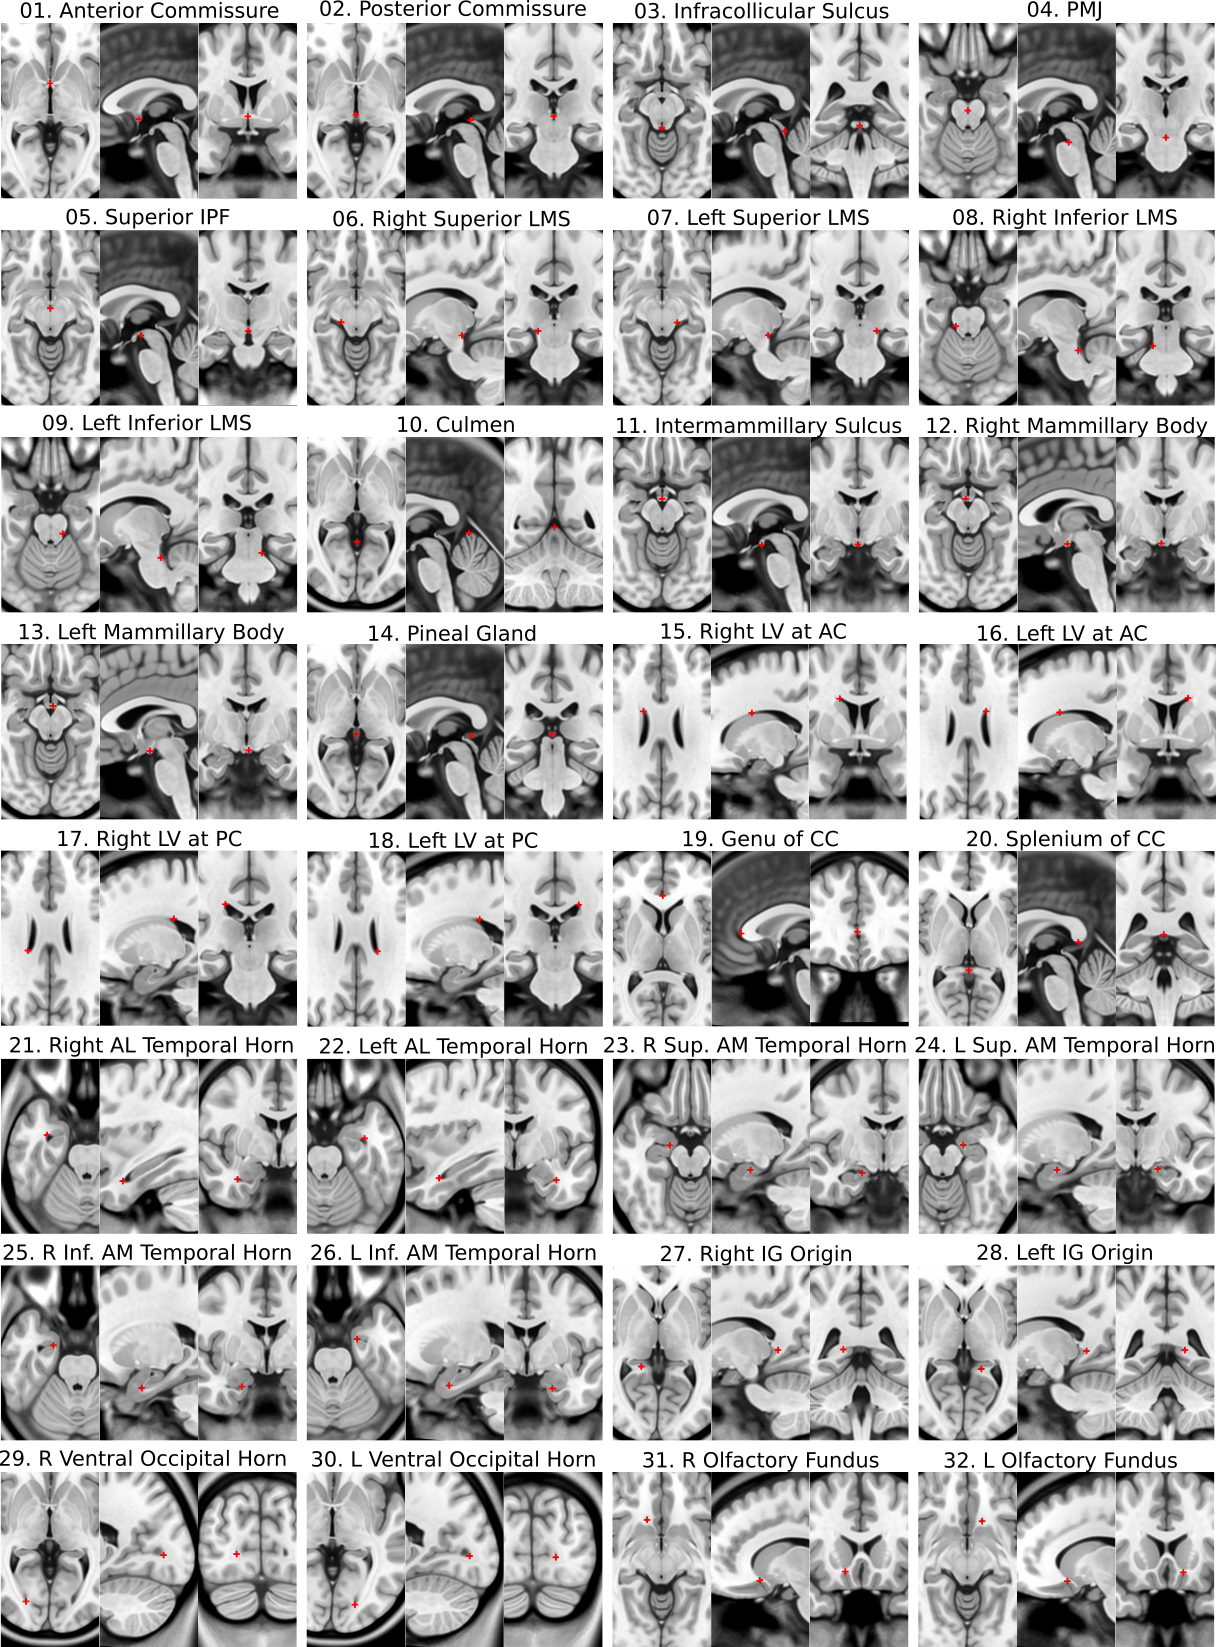
\includegraphics[width=0.8\linewidth]{figs/figuresupall_afids.png}
    \caption{The anatomical fiducials in the protocol is demonstrated with crosshairs at the representative location. AC, anterior commissure; AL, anterolateral; AM, anteromedial; IG, indusium griseum; IPF, interpeduncular fossa; LMS, lateral mesencephalic sulcus; LV, lateral ventricle; PC, posterior commissure; PMJ, pontomesenphalic junction.}
    \label{fig:figuresupall_afids}
\end{figure}


\newpage
\section{Rater Demographic Data}\label{app:rater_demo_data}
All annotations were performed by at least two human raters. As part of any annotation study, we collected demographic data on rater's experience in neuroanatomy, medical imaging, 3DSlicer software. Although not used in this paper, we also curated subthalamic nucelus (STN) segmentations on ultra-high field MRI (i.e., \(>\)7-T) data and add demographic rater data here for completeness. This data is used in Chapter \ref{chap:afidspred}. Table \ref{tab:rater_demographic_data} provides a breakdown of all the raters involved in datasets released in this work. 

\begin{table}[htbp]
\centering
\caption{
Summary of anatomical fiducial (AFID) and subthalamic nucleus (STN) annotation across datasets. Each row represents a unique annotator (Rater\_ID) contributing to one or more datasets. The table includes the experience (in months) of raters in three domains: Imaging, Neuroanatomy, and 3D Slicer. The diversity of rater backgrounds and annotation volumes reflects the breadth of participation across studies. Rater\_ID entries are context-specific and assigned uniquely within each dataset.
}
\begin{tabular}{llllll}
\toprule
Annotation & Dataset & Rater\_ID & Imaging & Neuroanatomy & 3DSlicer \\
\midrule
AFIDs & LHSCPD & AT & 0 & 0 & 0 \\
AFIDs & LHSCPD & GG & 60 & 60 & 60 \\
AFIDs & LHSCPD & MA & 60 & 60 & 60 \\
AFIDs & LHSCPD & MJ & 0 & 0 & 0 \\
AFIDs & LHSCPD & RC & 0 & 0 & 0 \\
AFIDs & AFIDs-HCP & AT & 60 & 60 & 60 \\
AFIDs & AFIDs-HCP & CZ & 12 & 12 & 12 \\
AFIDs & AFIDs-HCP & GG & 60 & 60 & 60 \\
AFIDs & AFIDs-HCP & DC & 24 & 24 & 24 \\
AFIDs & AFIDs-HCP & KF & 24 & 24 & 24 \\
AFIDs & SNSX32 & Rater01 & 12 & 12 & 12 \\
AFIDs & SNSX32 & Rater02 & 24 & 24 & 24 \\
AFIDs & SNSX32 & Rater03 & 24 & 24 & 24 \\
AFIDs & SNSX32 & Rater04 & 36 & 36 & 36 \\
AFIDs & SNSX32 & Rater05 & 24 & 24 & 24 \\
AFIDs & SNSX32 & Rater06 & 24 & 24 & 24 \\
AFIDs & SNSX32 & Rater07 & 24 & 24 & 24 \\
AFIDs & SNSX32 & Rater08 & 60 & 60 & 60 \\
AFIDs & SNSX32 & Rater09 & 12 & 12 & 12 \\
AFIDs & AFIDs-OASIS, MNI & Rater01 & 24 & 24 & 24 \\
AFIDs & AFIDs-OASIS, MNI & Rater02 & 0 & 0 & 0 \\
AFIDs & AFIDs-OASIS, MNI & Rater03 & 8 & 0 & 8 \\
AFIDs & AFIDs-OASIS, MNI & Rater04 & 24 & 6 & 0 \\
AFIDs & AFIDs-OASIS, MNI & Rater05 & 0 & 24 & 0 \\
AFIDs & AFIDs-OASIS, MNI & Rater06 & 24 & 12 & 12 \\
AFIDs & AFIDs-OASIS, MNI & Rater07 & 12 & 48 & 12 \\
AFIDs & AFIDs-OASIS, MNI & Rater08 & 0 & 0 & 0 \\
AFIDs & AFIDs-OASIS, MNI & Rater09 & 120 & 120 & 60 \\
AFIDs & 3T7T & Rater01 & 72 & 72 & 72 \\
AFIDs & 3T7T & Rater02 & 120 & 120 & 120 \\
AFIDs & 3T7T & Rater03 & 24 & 24 & 24 \\
AFIDs & 3T7T & Rater04 & 24 & 12 & 12 \\
AFIDs & 3T7T & Rater05 & 12 & 36 & 48 \\
AFIDs & 3T7T & Rater06 & 0 & 12 & 0 \\
STN & SNSX & Rater A & 120 & 120 & 60 \\
STN & SNSX & Rater B & 240 & 240 & 12 \\
STN & SNSX & Rater C & 72 & 72 & 72 \\
STN & 3T7T & Rater A & 84 & 84 & 84 \\
\bottomrule
\end{tabular}
\label{tab:rater_demographic_data}
\end{table}


\newpage
\chapter{Chapter 3 Supplementary Content}\label{app:ch3suppcontent}
\myappendices{Appendix \ref{app:ch3suppcontent}: Chapter 3 Supplementary Content}
\newpage

\section{AutoAFIDs Snakebids.yaml file}
\label{app:yaml}
The \texttt{snakebids.yaml} file defines user-facing options and input configurations for executing the AutoAFIDs workflow as a BIDS-App. While the file includes structural elements necessary for Snakebids compatibility, its most relevant components are those that control the behavior of the workflow based on user-defined parameters:
\begin{itemize}
  \item \textbf{\texttt{--modality}}: Specifies the input image type to process. Supported values include \texttt{T1w}, \texttt{T2w}, \texttt{FLAIR}, and \texttt{ct}. If this flag is not provided, \texttt{T1w} modality is run by default.
  
  \item \textbf{\texttt{--procprofile}}: Controls the preprocessing intensity. Options include \texttt{slow}, \texttt{medium}, \texttt{fast}, and \texttt{superfast}. The default is \texttt{fast}.
  
  \item \textbf{\texttt{--norm}}: Chooses the intensity normalization strategy. Options are \texttt{0} (z-score normalization) and \texttt{1} (min-max normalization).
  
  \item \textbf{\texttt{--res}}: Sets the target isotropic resolution for resampling (e.g., \texttt{100} for 1~mm). This allows the user to balance accuracy and runtime efficiency.
  
  \item \textbf{\texttt{--participant\_label}} and \textbf{\texttt{--exclude\_participant\_label}}: Control which BIDS subjects are included or excluded from the current run. Multiple subjects can be specified as a space-separated list.
  
  \item \textbf{\texttt{--stereotaxy}}: Enables prediction of stereotactic coordinates (e.g., for DBS targets). Supported options include \texttt{STN} and \texttt{cZI}. When specified, the workflow also outputs the associated AC–PC transform matrix. This feature implements the models built in Chapter \ref{chap:afidspred}.
  
  \item \textbf{\texttt{--fidqc}}: Toggles the generation of interactive HTML quality control reports for AFID placements. This is disabled by default but can be enabled with the \texttt{--fidqc} flag.
  
  \item \textbf{\texttt{--LEAD-DBS-DIR}} and \textbf{\texttt{--FMRIPREP-DIR}}: Allow integration with external derivatives from prior processing pipelines. If provided, AFID-based registration evaluation will be applied to these datasets.
  
  \item \textbf{\texttt{--workdir}}: Optionally specifies a working directory. This can be used to store intermediate files on high-speed scratch spaces (e.g., \texttt{\$SLURM\_TMPDIR}).
\end{itemize}

\begin{minted}[fontsize=\small, bgcolor=bg, linenos, breaklines]{yaml}
bids_dir: "/path/to/bids/dir"
output_dir: "/path/to/output/dir"
...
parse_args:
#---  core BIDS-app options ---
  bids_dir:
    help: The directory with the input dataset formatted according to the BIDS standard.
  
  output_dir:
    help: The directory where the output files should be stored. If you are running
      group level analysis this folder should be prepopulated with the results of
      the participant level analysis.
      
  analysis_level:
    help: Level of the analysis that will be performed
    choices: *analysis_levels

  --participant_label:
      help: The label(s) of the participant(s) that should be analyzed. The label
            corresponds to sub-<participant_label> from the BIDS spec (so it does
            not include "sub-"). If this parameter is not provided, all subjects
            will be analyzed. Multiple participants can be specified with a space
            seperated list.
      nargs: "+"

  --exclude_participant_label:
      help: The label(s) of the participant(s) that should be excluded. The label
            corresponds to sub-<participant_label> from the BIDS spec (so it does
            not include "sub-"). If this parameter is not provided, all subjects
            will be analyzed. Multiple participants can be specified with a space
            sepearated list.
      nargs: "+"

  --acq:
      help: 'The acquisition sequence of the T1w image (e.g. MP2RAGE). (default: %(default)s)'
      default: MP2RAGE
      nargs: "?"

  --procprofile:
      help: 'Specify the profile and configration for preprocessing. (default: %(default)s)'
      choices: ['slow','medium','fast','superfast']
      default: 'fast'

  --norm:
      help: 'Specify the normalization scheme for images as a binary choice. {0 = z-score, 1 = min-max , 2 = tissue-based [notavailable]}. (default: %(default)s)'
      choices: ['0', '1']
      default: '0'  # Default to 0, which represents z-score normalization

  --res:
      help: 'Specify the resampling resolution (e.g. "100" for 1mm) for images, any resolution is supported but limited to isotropic resampling. (default: %(default)s)'
      default: '100'  # Default to 1 
    
  --modality: 
      help: 'Specify the modality to use (e.g., T1w, T2w, FLAIR, or CT).'
      default: 'T1w'
      choices:
        - T1w
        - T2w
        - FLAIR
        - ct

  --derivatives:
      help: 'Path(s) to a derivatives dataset, for folder(s) that contains multiple
        derivatives datasets (default: %(default)s) '
      default: false
      nargs: +

  --model:
      help: 'Type of machine learning model to apply.'
      default: 'default'
      required: false

  --enable-bids-validation:
    help: |
      Enable validation of BIDS dataset. BIDS validation would be performed
      using the bids-validator plugin (if installed/enabled) or with the pybids
      validator implementation (if bids-validator is not installed/enabled).
    dest: "plugins.validator.skip"
    action: "store_false"
    default: True

  --stereotaxy:
    help: 'Predict stereotactic target coordinates from output AFIDs. Also supplies AC-PC transform matrix (4x4) in the process.{STN = subthalamic nucelus, cZI = caudal zona incerta}'
    choices: ['STN','cZI']
    default: false
    required: false

  --fidqc:
    help: 'Generate *.html files for QC of AutoAFIDs outputs. (default: %(default)s)'
    dest: "fidqc"
    action: "store_true"  # Automatically sets to True when flag is used
    default: false        # Default to False when not used

  --LEAD-DBS-DIR:
    help: 'Path to a LEAD-DBS derivatives dataset, for folder(s) that contains multiple derivatives datasets (default: %(default)s) '
    default: false
    required: false
    type: str

  --FMRIPREP-DIR:
    help: 'Path to a fMRIPrep derivatives dataset, for folder(s) that contains multiple derivatives datasets (default: %(default)s) '
    default: false
    required: false
    type: str

  --workdir:
    help: |
      Folder for storing working files. If not specified, will be in "work/" subfolder 
      in the output folder. You can also use environment variables when setting the 
      workdir, e.g. --workdir '$SLURM_TMPDIR'.
    default: work
    type: str

#--- workflow specific configuration ---

# Nifti template
templatet1w: 'resources/tpl-MNI152NLin2009cAsym_res-01_T1w.nii.gz'
templatet1w_lead: 'resources/tpl-MNI152NLin2009bAsym_res-01_T1w.nii.gz'

# AFIDs fcsv template
fcsv: 'resources/dummy.fcsv'
fcsv_mni: 'resources/tpl-MNI152NLin2009cAsym_res-01_desc-groundtruth_afids.fcsv'
fcsv_mni_lead: 'resources/tpl-MNI152NLin2009bAsym_res-01_desc-groundtruth_afids.fcsv'

singularity:
  synthstrip: 'docker://freesurfer/synthstrip:1.3'
  synthsr: 'docker://mackenzieasnyder/synthsr:latest'

# It will be downloaded to ~/.cache/autoafids
resource_urls:
  default: 'files.osf.io/v1/resources/9fptg/providers/osfstorage/?zip='

#Stereotaxy models 
STN: 'resources/stereotaxy/STN.pkl'
cZI: 'resources/stereotaxy/cZI.pkl'
template_fcsv: 'resources/stereotaxy/target_template.fcsv'
...
\end{minted}

\newpage
\section{Prediction Accuracy across all landmarks}

\begin{table}[H]
\centering
\footnotesize
\caption{Landmark prediction accuracy of AutoAFIDs. Values represent the Euclidean Distance (ED) between predicted and ground truth landmark coordinates across 21 test subjects.} \label{tab:autoafids_accuracy}
\begin{tabular}{lcccc}
\toprule
\textbf{Landmark} & \textbf{Median (mm)} & \textbf{IQR (mm)} & \textbf{Min (mm)} & \textbf{Max (mm)} \\
\midrule
AFID 1 & 0.42 & 0.29--0.69 & 0.04 & 1.53 \\
AFID 2 & 0.83 & 0.73--1.14 & 0.37 & 1.32 \\
AFID 3 & 0.90 & 0.65--1.09 & 0.36 & 2.06 \\
AFID 4 & 0.73 & 0.58--0.95 & 0.15 & 2.08 \\
AFID 5 & 0.80 & 0.60--1.12 & 0.29 & 2.46 \\
AFID 6 & 1.57 & 1.04--1.78 & 0.42 & 2.37 \\
AFID 7 & 1.26 & 0.86--1.55 & 0.24 & 2.39 \\
AFID 8 & 1.67 & 1.20--2.67 & 0.52 & 3.99 \\
AFID 9 & 1.41 & 1.07--2.43 & 0.51 & 3.99 \\
AFID 10 & 1.47 & 1.16--2.29 & 0.69 & 3.37 \\
AFID 11 & 0.72 & 0.48--0.84 & 0.25 & 1.23 \\
AFID 12 & 0.64 & 0.43--0.83 & 0.35 & 1.29 \\
AFID 13 & 0.93 & 0.68--1.11 & 0.38 & 1.60 \\
AFID 14 & 0.93 & 0.79--1.40 & 0.32 & 3.85 \\
AFID 15 & 2.00 & 0.97--3.30 & 0.26 & 5.28 \\
AFID 16 & 2.34 & 1.67--3.28 & 0.96 & 4.62 \\
AFID 17 & 2.38 & 1.19--2.61 & 0.32 & 3.99 \\
AFID 18 & 1.04 & 0.85--1.52 & 0.17 & 2.96 \\
AFID 19 & 1.27 & 1.02--1.56 & 0.14 & 2.83 \\
AFID 20 & 0.89 & 0.71--1.14 & 0.37 & 2.76 \\
AFID 21 & 1.32 & 0.70--1.73 & 0.47 & 4.03 \\
AFID 22 & 1.31 & 1.02--1.75 & 0.47 & 3.49 \\
AFID 23 & 1.16 & 0.53--1.69 & 0.10 & 3.31 \\
AFID 24 & 2.28 & 1.53--2.67 & 0.35 & 4.12 \\
AFID 25 & 2.28 & 1.66--3.04 & 0.64 & 3.59 \\
AFID 26 & 2.08 & 1.45--2.94 & 1.15 & 4.22 \\
AFID 27 & 1.47 & 0.80--2.10 & 0.21 & 3.46 \\
AFID 28 & 1.56 & 1.21--1.87 & 0.55 & 3.36 \\
AFID 29 & 1.79 & 1.38--2.46 & 0.70 & 3.61 \\
AFID 30 & 2.21 & 1.18--2.78 & 0.35 & 3.96 \\
AFID 31 & 1.19 & 0.91--1.63 & 0.34 & 2.98 \\
AFID 32 & 1.00 & 0.79--1.69 & 0.12 & 2.64 \\
\midrule
\textbf{All AFIDs} & \textbf{1.21} & \textbf{0.76--1.95} & \textbf{0.04} & \textbf{5.28} \\
\bottomrule
\end{tabular}
\end{table}

\newpage
\section{Registration quality control file}
\label{app:registrationqualitycontrol}
AutoAFIDs provides an optional registration quality control (QC) module that generates subject-level HTML reports to assess the fidelity of spatial normalization. For each subject, the tool computes standard summary statistics of landmark error, including minimum, maximum, mean, median, standard deviation, and interquartile range across all 32 anatomical fiducials. Visualizations include (i) slice-based qualitative review panels with crosshair overlays in sagittal, coronal, and axial views, (ii) a color-coded heatmap of per-landmark errors across x, y, z axes and Euclidean distance, and (iii) a 3D scatterplot showing the displacement between predicted subject landmarks and reference coordinates in stereotactic space. The report enables both quantitative inspection and visual verification of anatomical alignment and can be integrated into larger processing workflows for automated QC flagging.

The registration QC module in AutoAFIDs can be invoked as part of the BIDS-App command-line interface. To enable QC report generation, users must provide a directory containing their Lead-DBS derivative files. A typical invocation is shown below:

\begin{minted}[fontsize=\small, bgcolor=bg, linenos, breaklines]{bash}
autoafids <BIDS_DIR> <DERIVATIVES_DIR> participant --LEAD-DBS-DIR <PATH_TO_LEAD-DBS_Directory>
\end{minted}

This command runs the QC module on all subjects found in the BIDS directory, compares registered AFIDs to reference space, and saves the resulting HTML reports to the specified output directory. Each report includes per-subject error statistics, slice-wise visual inspection panels, a heatmap of landmark errors, and a 3D displacement plot. This functionality is integrated into the default workflow and designed for seamless use in automated pipelines.
\newpage

\chapter{Chapter 4 Supplementary Content}\label{app:suppcontentch4}
\myappendices{Appendix \ref{app:suppcontentch4}: Chapter 4 Supplementary Content}
\newpage

\section{Quality Control}\label{app:qualitycontrol}
All annotations were quality controlled by AT, JZ, and EC. To facilitate ease of review, a QC interface was created in the form of an HTML file format. This QC file was generated for all the participants in the dataset and contains all annotations (e.g., AFIDs or STN) performed for that subject. We make all QC files availible in: \url{https://github.com/afids/afids-pred/tree/main/data/QC}.

\begin{figure}[hbt!]
    \centering
    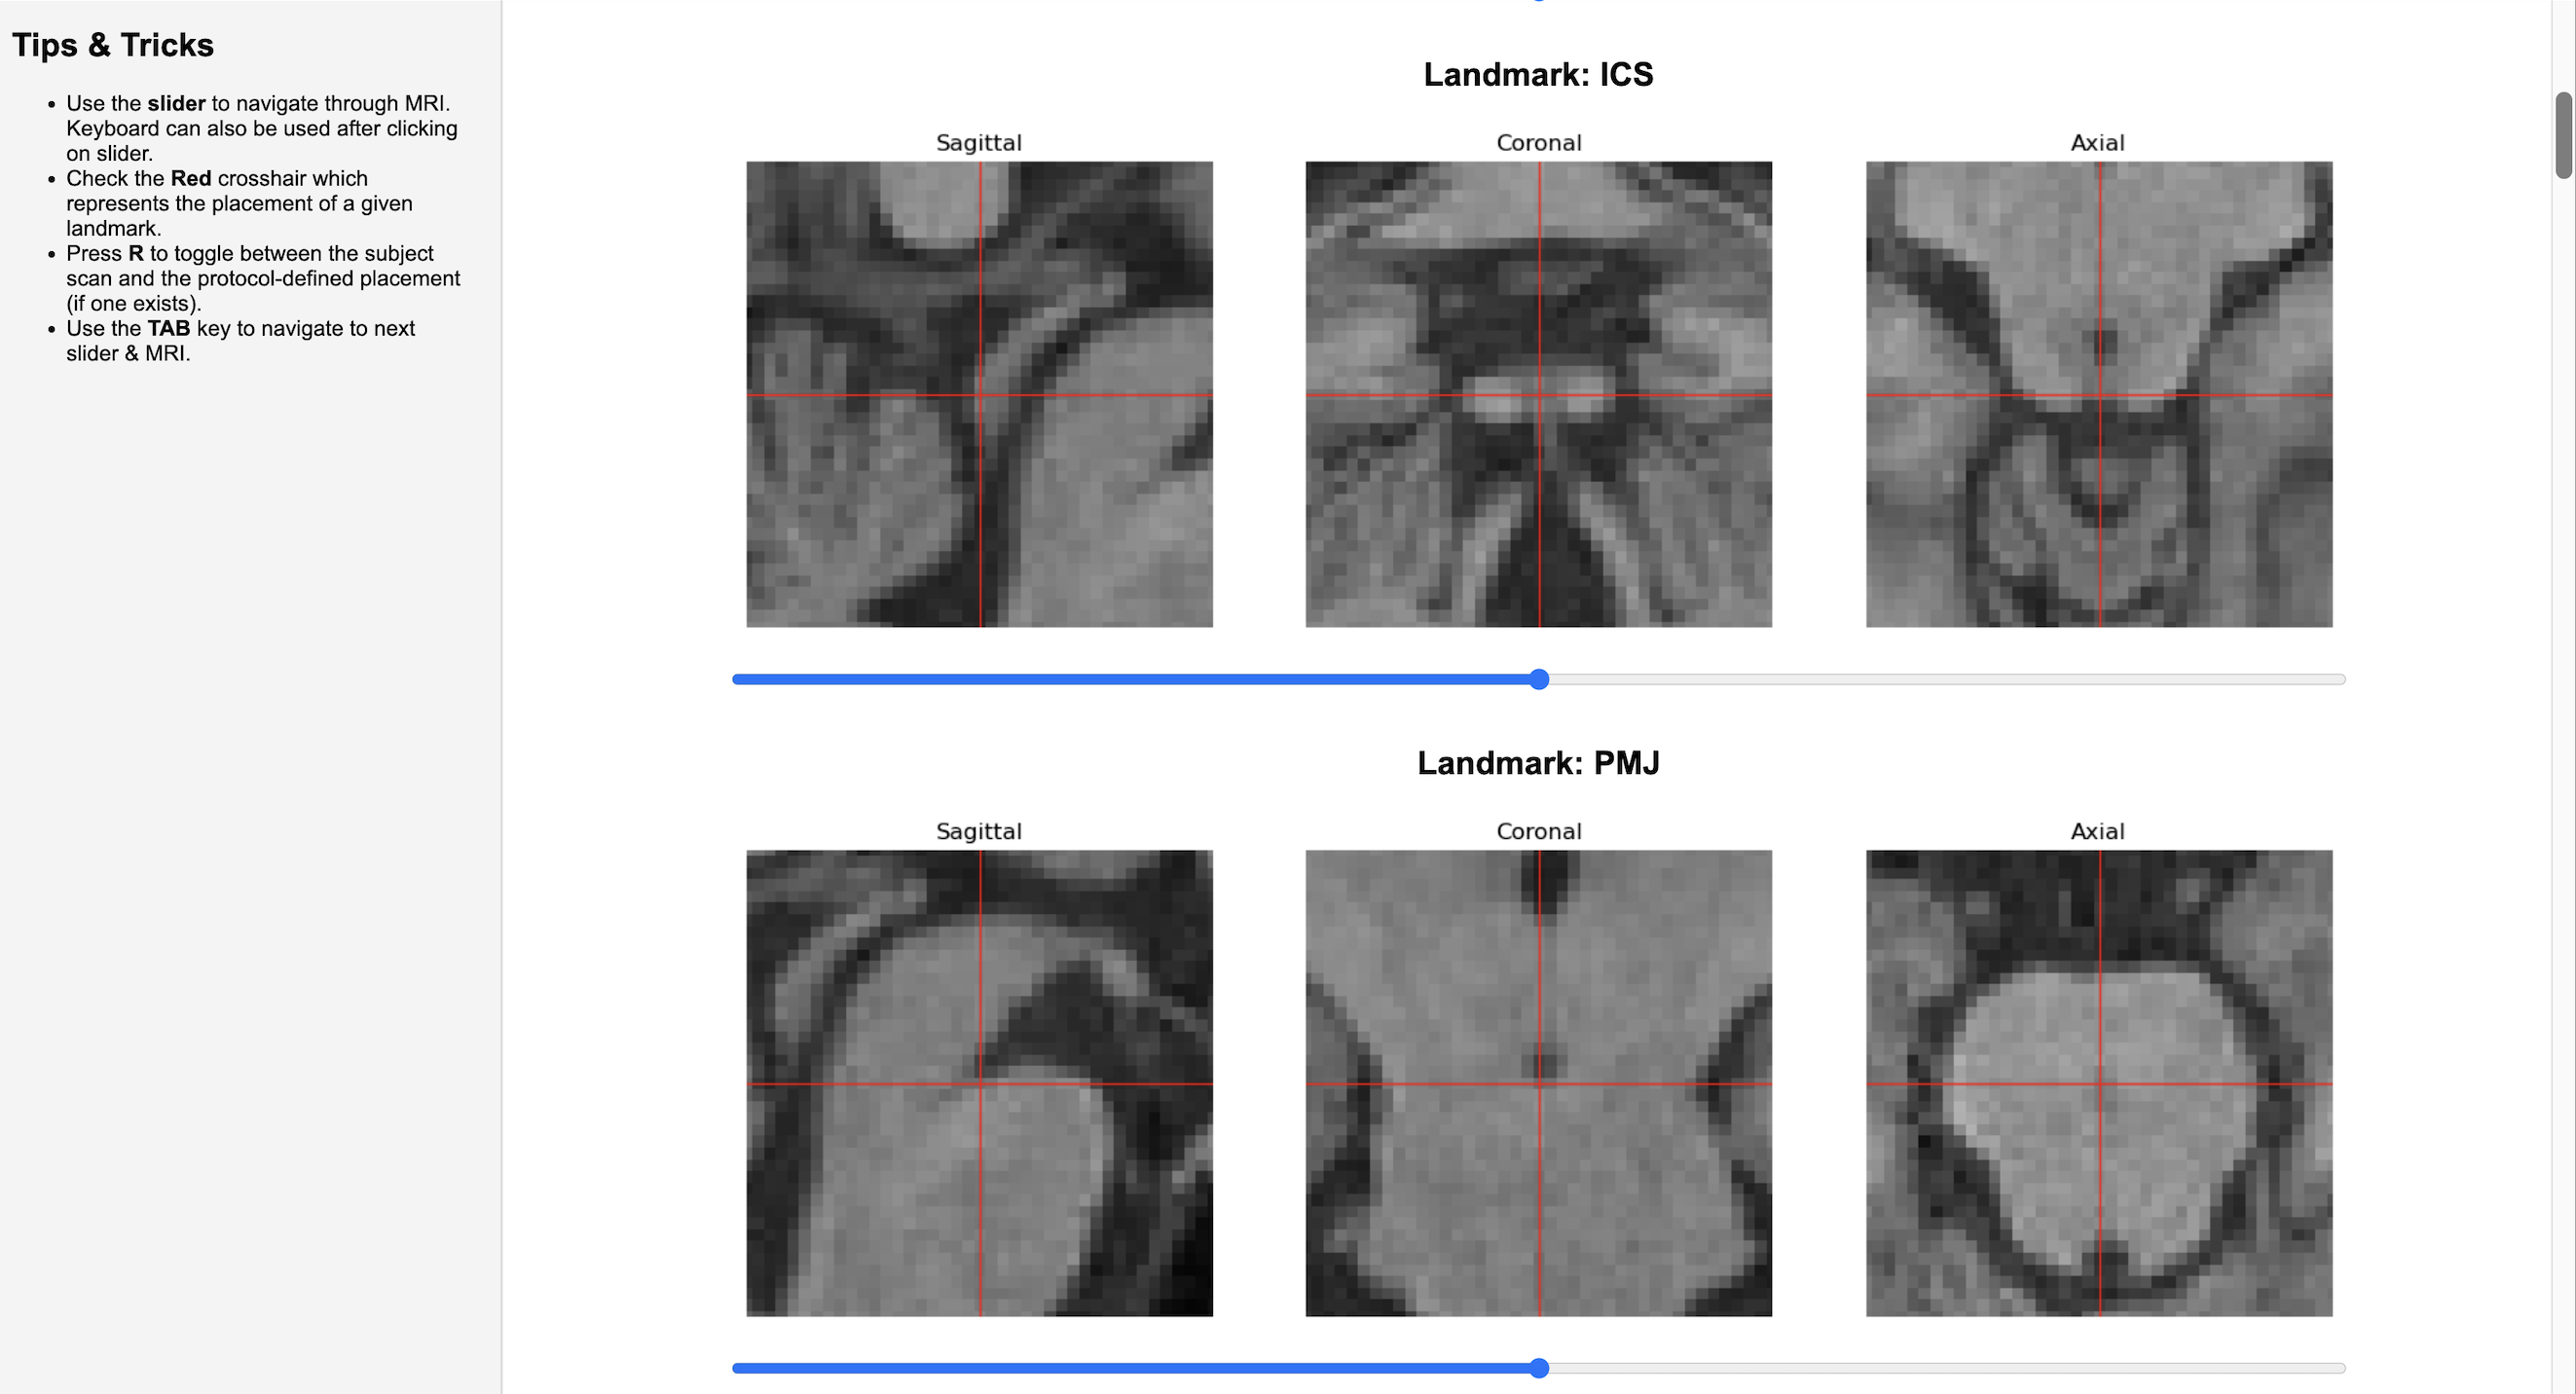
\includegraphics[width=0.95\linewidth]{figs/figuresupQC.png}
    \caption{Quality control visualization for anatomical landmark placement. Crosshairs indicate the annotated location of an example fiducial (the infracollicular sulcus [ICS]) in sagittal, coronal, and axial MRI views. Reviewers can toggle between the subject scan and the protocol-defined (template) annotation using the R key while navigating select slices in MRI volume using arrowkeys or slider.}
    \label{fig:figuresupQC}
\end{figure}
\chapter{Ethics Approvals}\label{app:ethics}
\myappendices{Appendix \ref{app:ethics}: Ethics Approvals}

\newpage
\section{Ethics 1}\label{app:ethics:reb_details}
\begin{figure}[h]
	\centering
	%\includegraphics[width=.825\textwidth]{EthicsChapter_details.pdf}
\end{figure}

\newpage
\section{Ethics 2}\label{app:ethics2}
\begin{figure}[h]
	\centering
	%\includegraphics[width=.825\textwidth]{EthicsChapter_details2.pdf}
\end{figure}

\chapter{Copyright Transfers and Reprint Permissions}\label{app:copyright}
\myappendices{Appendix \ref{app:copyright}: Copyright Transfers and Reprint Permissions}

The reprint permissions for the following accepted articles are provided:
\begin{itemize}
	\item Accepted Manuscript 1 details.
	\item Accepted Manuscript 2 details.
\end{itemize}
All other copyright material is under sole ownership by the author, including arXiv pre-prints, and articles currently under submission or revision.

% TODO: get CopyrightTransfer info
%\includepdf[pages={1-6}]{CopyrightTransfer_accepted_manuscript1.pdf}
%\includepdf[pages={1-2}]{CopyrightTransfer_accepted_manuscript2.pdf}
\end{appendices}
\newpage
\singlespacing

%% This adds a line for the Bibliography in the Table of Contents.
\phantomsection
\addcontentsline{toc}{chapter}{Bibliography}
%% ***   Set the bibliography style.   ***
\bibliographystyle{apalike} % (change according to your preference)
%%% ***   Set the bibliography file.   ***
\bibliography{paperpile}
%% ***   NOTE   ***
%% If you don't use bibliography files, comment out the previous line
%% and use \begin{thebibliography}...\end{thebibliography}.  (In that
%% case, you should probably put the bibliography in a separate file
%% and \include or \input it here).

\clearpage
\pagestyle{plain}
% CV section (add hyperlink to ToC)
\newpage % Optional: Add a new page for the CV section
\phantomsection % For correct hyperlinking
\addcontentsline{toc}{chapter}{Curriculum Vitae}
\section*{\textsc{Curriculum Vitae}}

\section*{\textsc{Education}} \noindent\hrulefill \vspace{0.5em}
\begin{tabularx}{\textwidth}{@{}X r@{}}
\textbf{Doctor of Medicine (MD)}, \textsc{Stanford University} & \textit{Aug 2025 – Jun 2029} \\
\textbf{PhD in Biomedical Engineering}, \textsc{Western University} & \textit{Sep 2021 – Aug 2025} \\
\textbf{BMSc in Interdisciplinary Medical Sciences}, \textsc{Western University} & \textit{Sep 2017 – Jun 2021} \\
\end{tabularx}

\vspace{0.5em}
\section*{\textsc{Honors and Awards}} \noindent\hrulefill \vspace{0.5em}
% \begin{itemize}
  \item \textbf{Merit Abstract Award}, OHBM (International, 2024) \hfill \textit{\$1,000}
  \item \textbf{Parkinson Canada Graduate Student Award} (National, 2024) \hfill \textit{\$40,000}
  \item \textbf{NSERC CGS-D}, Canada Graduate Scholarship (National, 2023) \hfill \textit{\$120,000}
  \item \textbf{Mitacs Accelerate Fellowship} (National, 2022) \hfill \textit{\$25,000}
  \item \textbf{Ontario Graduate Scholarship} (Provincial, 2022 \& 2023) \hfill \textit{\$15,000 each}
  \item \textbf{Parkinson’s SWO Studentship} (Provincial, 2022) \hfill \textit{\$25,000}
  \item \textbf{Best Abstract}, Canadian Neuromodulation Conference (2022) \hfill \textit{\$1,500}
  \item \textbf{Best Platform Talk}, Clinical Neurological Research Day (2023) \hfill \textit{\$1,000}
  \item \textbf{Rising Youth Community Service Award} (National, 2020) \hfill \textit{\$5,000}

% \end{itemize}

\vspace{0.5em}
\section*{\textsc{Positions and Leadership}} \noindent\hrulefill \vspace{0.5em}
% \begin{itemize}
  \item \textbf{Co-Founder \& Board Member} — \href{https://webstraw.ca}{WebStraw}
  \item \textbf{Co-Founder \& Board Member} — \href{https://refuhope.com}{RefuHope}
  \item \textbf{Editor} — \href{https://stimulatingbrains.org}{Stimulating Brains Podcast}
  \item \textbf{Facilitator} — Deep Brain Stimulation Patient Support Group
  \item \textbf{Chair} — Biomedical Engineering Graduate Student Committee
  \item \textbf{Representative} — Schulich School of Medicine and Dentistry Committee
  \item \textbf{Representative} — Society of Graduate Students
  \item \textbf{Teaching Assistant} — Undergraduate Engineering (Years 1–2)
% \end{itemize}

\vspace{0.5em}
\section*{\textsc{Peer-Reviewed Publications}} \noindent\hrulefill \vspace{0.5em}
% \begin{enumerate}
  \item Abbass M., Taha A., Gilmore G., et al. (2024). \textit{Quantifying localization and registration accuracy using anatomical fiducials: application to deep brain stimulation}. \textit{Imaging Neuroscience}, In press.
  \item Haast R.M., Kai J., Taha A., et al. (2024). \textit{Mapping the topographic organization of the human zona incerta using diffusion MRI}. \textit{eLife}, 14:RP103530.
  \item Ogunsanya F., Taha A., et al. (2023). \textit{MRI-degad: Towards accurate conversion of gadolinium-enhanced MRI to non-contrast-enhanced scans via CNNs}. \textit{Int J CARS}, 19, 1469.
  \item Taha A., et al. (2023). \textit{Magnetic resonance imaging datasets with anatomical fiducials for quality control and registration}. \textit{Sci Data}, 10, 449.
  \item Taha A., Gilmore G., Khan A., Lau J.C. (2022). \textit{An indirect deep brain stimulation targeting tool using salient anatomical fiducials}. \textit{Neuromodulation}, 25(6).
  \item Abbass M., Gilmore G., Taha A., et al. (2022). \textit{Application of anatomical fiducials to a clinical dataset of Parkinson’s disease patients}. \textit{Brain Struct Funct}, 227, 393–405.
  \item Elias G.J.B., Germann J., Loh A., Boutet A., Taha A., et al. (2022). \textit{Normative connectomes and their use in DBS}. In A. Horn (Ed.), \textit{Connectomic Deep Brain Stimulation} (pp. 245–274). Academic Press.
  \item Germann J., Mameli M., Elias G.J.B., Loh A., Taha A., et al. (2021). \textit{Deep brain stimulation of the habenula: Systematic review and clinical trial registries}. \textit{Front Psychiatry}, 12, 730931.
  \item Boutet A., Loh A., Chow C., Taha A., et al. (2021). \textit{Advancements in MRI sequences for visualizing functional neurosurgical targets}. \textit{J Neurosurg}, 1–14.
% \end{enumerate}
\vspace{0.5em}
\section*{\textsc{Conference Presentations}} \noindent\hrulefill \vspace{0.5em}
% \begin{enumerate}
    \item Taha A. et al. (2025). AutoAFIDs: BIDS App for landmark detection, QC, stereotactic targeting and brain charting. \textit{OHBM}, Oral (International).
    \item Taha A. et al. (2024). Bridging brain coordinates and machine learning for surgical targeting and morphometric mapping. \textit{OHBM}, Oral (International).
    \item Taha A. et al. (2023). Mapping the subcortical connectome in Parkinson’s disease using 7-Tesla diffusion MRI. \textit{OHBM}, Poster (International).
    \item Taha A. et al. (2023). Open software infrastructure for automatic brain landmark localization for neuroimaging applications. \textit{OHBM}, Poster (International).
    \item Taha A. et al. (2023). Localizing the subthalamic nucleus using validated anatomical landmarks and machine learning. \textit{OHBM}, Poster (International).
    \item Kai J., Haast R.A.M., Taha A. et al. (2023). Cortical connections of the zona incerta revealed by in vivo diffusion. \textit{OHBM}, Poster (International).
    \item Gilmore G., Taha A. et al. (2022). Retrospective analysis of factors impacting SEEG accuracy at a Canadian center. \textit{American Epilepsy Society}, Poster (International).
    \item Taha A. et al. (2022). Deep brain stimulation targeting using an open-access anatomical fiducial framework. \textit{Imaging Network Ontario}, Oral (Provincial).
    \item Taha A. et al. (2022). Localizing the subthalamic nucleus on T1w gadolinium-enhanced imaging. \textit{Neuroscience Research Day}, Oral (Provincial).
% \end{enumerate}


\end{document}